\documentclass[12pt,a4paper]{scrreprt}
\usepackage[utf8]{inputenc}
\usepackage{geometry}
\geometry{
  left=3cm,
  right=2cm,
  bindingoffset=0mm
}
\usepackage[german]{babel}
\usepackage[scaled]{helvet}
\usepackage[T1]{fontenc}
\usepackage[footnote]{acronym}
\usepackage{amsmath}
\usepackage{textcomp}
\usepackage{amsfonts}
\usepackage{amssymb}
\usepackage{graphicx}
\usepackage{xcolor}
\usepackage{float}
\usepackage[onehalfspacing]{setspace}
\usepackage{hyperref}
\usepackage{titling}
%\usepackage[headsepline]{scrlayer-scrpage}
\usepackage{empheq}
\usepackage{longtable}
%\usepackage{subfigure}
\usepackage{subcaption}
\usepackage{ulem}
\usepackage{pdfpages}
\usepackage{soul}
\usepackage{import}
\usepackage[style=numeric, block=ragged]{biblatex}
\usepackage{etoolbox}
\usepackage{hyperref}
\usepackage{multirow}
\usepackage{multicol}
\usepackage{tabularx}
\usepackage{colortbl}
\usepackage{extarrows}
% \usepackage{subfigure}
% \usepackage{subcaption}



\apptocmd{\UrlBreaks}{\do\f\do\m}{}{}
\setcounter{biburllcpenalty}{9000}% Kleinbuchstaben
\setcounter{biburlucpenalty}{9000}% Großbuchstaben
\addbibresource{Literatur.bib}

%Kürzen in Formel
\usepackage{tikz}
    \usetikzlibrary{shapes}
    \usetikzlibrary{plotmarks}

\newcommand{\cancelb}[2][black]{%
\begin{tikzpicture}[inner sep=0pt, outer sep=0pt]
\node[](TEXT) {${\smash[b]{#2}}$};
\draw[#1, thick, shorten >=-1.5pt, shorten < = -1.5pt] (TEXT.west) -- (TEXT.east);
\end{tikzpicture}
}%

    


%Zitationsstil
%\bibliographystyle{IEEEtran}

%bei itemize Aufzählung --> Sternchen und nicht Bullet (dicker Punkt)
%\renewcommand*\labelitemi{\textasteriskcentered}

%Seitenzahlen unten rechts
\usepackage{fancyhdr}
% Turn on the style
\pagestyle{fancy}
% Clear the header and footer
\fancyhead{}
\fancyfoot{}
% Set the right side of the footer to be the page number
\fancyfoot[R]{\thepage}

\makeatletter
\renewcommand\chapter{\if@openright\cleardoublepage\else\clearpage\fi
					\thispagestyle{fancy}%
					\global\@topnum\z@
					\@afterindentfalse
					\secdef\@chapter\@schapter}


\usepackage{xcolor}
\usepackage{listings}
\lstset{basicstyle=\ttfamily,
  showstringspaces=false,
  commentstyle=\color{red},
  keywordstyle=\color{blue}
}
\newcommand*\downs[1]{\mathop{\downarrow}\limits_{\mathclap{#1}}}

\newcommand*{\quelle}{% 
  \footnotesize Quelle: 
} 

%Wenn Kopfzeile erwünscht ist, siehe Vergleich Projektarbeit auf den einzelnen Seiten, dann wieder einkommentieren

%Kopfzeile
%\pagestyle{headings}
%\automark[section]{chapter}
%\ihead[]{\includegraphics[width=0.3\textwidth]{Bilder/ThLogo.png}}
%\chead{\headmark}
%\ohead[]{Abschlussarbeit}

\setcounter{secnumdepth}{4} % how many sectioning levels to assign numbers to
\setcounter{tocdepth}{4}    % how many sectioning levels to show in ToC
%\title{Titel der Arbeit}
%\author{
 % Name, Nachname
%  \textit{Matrikelnummer: ???????? }\\
%}



\begin{document}
%Leere Seite zu Beginn
%\newpage\thispagestyle{empty}~
\pagenumbering{Roman}
%----------------------------------------------------------------------------------------------
%Titelseite
\begin{titlepage}
    \begin{center}
  	Technische-Hochschule Nürnberg\\
Fakultät Elektrotechnik Feinwerktechnik Informationstechnik\\
\ \\
Studiengang Master Elektronische und Mechatronische Systeme (M-SY)\\
\ \\
\large\textbf{Masterarbeit}\\
von \\
Firat \so{G\"ok}\\ %Nachname gesperrt formatiert
\ \\
{\large\textbf{Programmierung eines mobilen Roboters für die autonome Navigation in einem benutzerdefinierten Hindernisparcours und das dafür entwickelte API}}\\
\ \\
\ \\
Wintersemester 2021/22\\
Abgabedatum: 14.02.2022\\
%Sommersemester 2021 \\
\ \\
\ \\
\ \\  
    
    \end{center}
\ \\
\ \\
\ \\
% \ \\
%\ \\
%\ \\

\begin{tabular}{p{8cm}p{7cm}}\\
Betreuer: & \\
Prof. Dr. Stefan May & Dipl.-Ing. Karlheinz Ruff \\
Prof. Dr. Jörg Arndt & Kurt H\"uttinger GmbH \& Co. KG.\\
\end{tabular}

\begin{labeling}{Schlagworte:}
\item[Schlagworte:] mobile Robotik, autonomer mobiler Roboter, ROS, autonom, autonom Navigation, rospy, Pledge-Algorithmus 
\end{labeling}

%\end{tabular}
%\begin{labeling}{Betreuer:}
%%\item[Abgabedatum:] 05.07.2021
%\item[Betreuer:] Prof. Dr. Stefan May \\
%Prof. Dr. Jörg Arndt
%\end{labeling}


\end{titlepage}
%-----------------------------------------------------------------------------------------------


%---------------------------------------------------------------------------------------------
%Prüfungsrechtliche Erklärung des Studierenden "Erklärung gemäß §19 (8) APO"
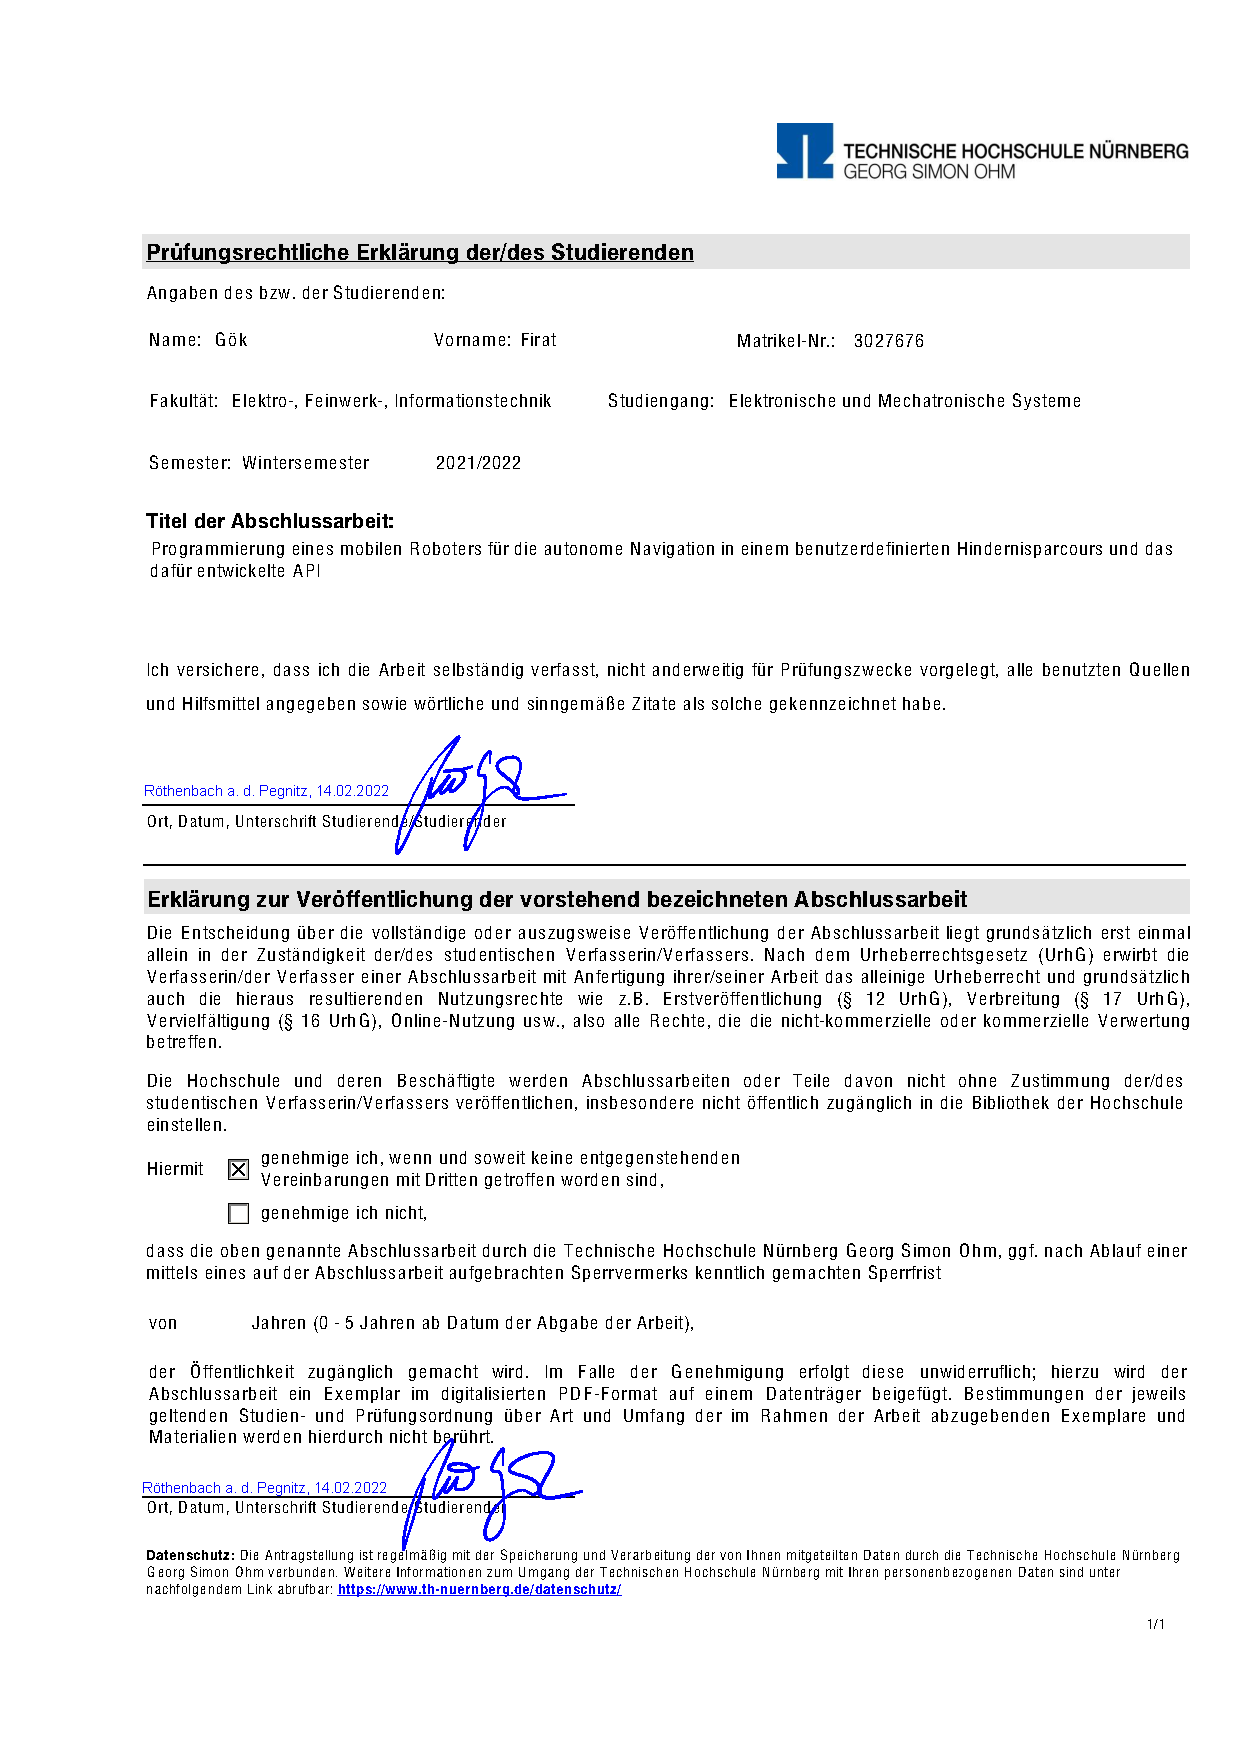
\includepdf[pages=1, scale=1.0, frame=true]{PDFs/Firat_Goek_Pruefungsrechtliche_Erklaerung_zur_Abschlussarbeit_signed.pdf}
%-------------------------------------------------------------------------------------------

\section*{Kurzfassung}
\addcontentsline{toc}{chapter}{Kurzfassung}
Die vorliegende Arbeit soll die Umsetzung eines Exponates für Bildungseinrichtungen mit einem mobilen Roboter als Intelligenzträger untersuchen und entwickeln. Dazu wurde im Laufe der Arbeit eine API entwickelt, das als Bindeglied zwischen der Anwendung und der Roboterkontrollarchitektur dient. Hierbei wurde das System mit Intelligenz angereichert, um so die Fähigkeiten und Klugheiten der mobilen Roboter, die heute möglich sind, spielerisch zu transportieren. So wurde mithilfe von Sensoren eine Hinderniserkennung implementiert, um vorrangig sicherheitsrelevante Fähigkeiten hardwarenah abzuwickeln, aber es wurde auch ein Ansatz für einen Algorithmus entwickelt, der ermöglicht, den Roboter aus einem Labyrinth zu befreien. Durch die offene Gestaltung der API kann die grafische Benutzeroberfläche je nach Einrichtung und Zweck angepasst werden. Das System selbst, das in dieser Arbeit untersucht und experimentell entwickelt wurde, beinhaltet viele kleinere Subsysteme, die im Einzelnen verschiedene Funktionalitäten ermöglichen. Durch diese Arbeit konnte ein Wissenslevel erarbeitet werden, um so ein System für die Firma Kurt Hüttinger GmbH \& Co. KG zu entwickeln und gegebenenfalls mit weiteren Intelligenzen zu erweitern. 
\section*{Abstract}
\addcontentsline{toc}{chapter}{Abstract}
This thesis aims to investigate and develop the implementation of an exhibit for educational institutions using a mobile robot as an intelligence carrier. For this purpose, an API was developed during the course of the work, which serves as a link between the application and the robot control architecture. In this process, intelligence was added to the system in order to playfully convey the capabilities and smarts of mobile robots that are possible today. For example, obstacle detection was implemented using sensors to handle primarily safety-related capabilities in hardware, but an approach was also developed for an algorithm that allows the robot to escape from a maze. Due to the open design of the API, the graphical user interface can be customized depending on the setup and purpose. The system itself, which was studied and experimentally developed in this work, includes many smaller subsystems that individually enable different functionalities. Through this work a level of knowledge could be worked out to develop such a system for the company Kurt Hüttinger GmbH \& Co. KG and to extend it with further intelligences if necessary.
\section*{Danksagung}
\addcontentsline{toc}{chapter}{Danksagung}

An diese Stelle möchte ich die Gelegenheit nutzen, einigen Menschen zu danken, die mich in meinem Studium unterstützt und somit diese Masterarbeit erst möglich gemacht haben.\\

Mein erster Dank gilt Herrn Prof. Dr. Stefan May, der diese Abschlussarbeit betreut und unterstützt hat. Für die hilfreichen Anregungen und die konstruktive Kritik bei der Erstellung dieser Arbeit möchte ich mich herzlich bedanken. Ich bedanke mich auch für die Roboterlösung, die ich zur Verfügung gestellt bekommen habe. Des Weiteren möchte ich der Firma Hüttinger danken, für ihre Aufgeschlossenheit und ihre unbürokratische Hilfe. Außerdem möchte ich Frau Ammon für das Korrekturlesen meiner Masterarbeit danken. Ein besonderer Dank gilt meinen Eltern, die mir mit ihrer Unterstützung mein Studium erst ermöglicht haben, ohne dies an Bedingungen zu knüpfen.


%Inhaltsverzeichnis
\tableofcontents 

\newpage
%----------------------------------------------------------------------------------------------
%Abkürzungsverzeichnis
\section*{Abkürzungsverzeichnis}
\addcontentsline{toc}{chapter}{Abkürzungsverzeichnis}

\begin{longtable}[l]{p{2cm} l}

API 				& Application Programming Interface                         \\
                    &                                                           \\
ROS 				& Roboter Operating System                                  \\
                    &                                                           \\
DNS                 & Domain-Name-System                                        \\
                    &                                                           \\
IP				    & Internet Protocol                                         \\
                    &                                                           \\
TCP				    & Transmission Control Protocol                             \\
                    &                                                           \\
UDP				    & User Datagram Protocol                                    \\
                    &                                                           \\
LiDAR               & Light detection and ranging                               \\
                    &                                                           \\
IMU                 & Inertial Measurement Unit                                 \\
                    &                                                           \\
MINT                &  Mathematik, Informatik, Naturwissenschaft und Technik    \\
                    &                                                           \\
% SDK                 & Software Development Kit              \\
%                     &                                       \\
% STM                 & ST-Microelectronics                   \\
%                     &                                       \\


\end{longtable}


%---------------------------------------------------------------------------------------------
\newpage


%------------------------------------------------------------------------------------------------
%Formelzeichen und Abkürzungsverzeichnis
\addcontentsline{toc}{chapter}{Formelzeichen und Indizes}
\section*{Formelzeichen und Indizes}
\begin{longtable}[l]{p{2cm} l}

$\boldsymbol{s}$                & Strecke	                                        \\
					            &									                \\
$\boldsymbol{t}$                & Zeit                                              \\
					            &									                \\
$\boldsymbol{D}$                & Distanz oder Strecke	                            \\
					            &									                \\
$\boldsymbol{f}$                & Frequenz oder Brennweite	                        \\
					            &									                \\
$\boldsymbol{\lambda}$          & Wellenlänge                                       \\
					            &									                \\
$\boldsymbol{b}$                & Parallaxe                                         \\
					            &									                \\
$\boldsymbol{x_{t+1}}$          & x-Position zum Zeitpunkt t+1	                    \\
					            &									                \\
$\boldsymbol{y_{t+1}}$          & y-Position zum Zeitpunkt t+1	                    \\
					            &									                \\
$\boldsymbol{\theta_{t+1}}$     & Orientierung zum Zeitpunkt t+1	                \\
					            &									                \\
$\boldsymbol{x_{t}}$            & x-Position zum Zeitpunkt t	                    \\
					            &									                \\
$\boldsymbol{y_{t}}$            & y-Position zum Zeitpunkt t	                    \\
					            &									                \\
$\boldsymbol{\theta_{t}}$       & Orientierung zum Zeitpunkt t	                    \\
					            &									                \\
$\boldsymbol{\Delta U_{t}}$     & Positionsänderung zum Zeitpunkt t	                \\
					            &									                \\
$\boldsymbol{v_{current}}$      & Aktuelle Geschwindigkeit	                        \\
					            &									                \\
$\boldsymbol{v_{max}}$          & Maximale Geschwindigkeit	                        \\
					            &									                \\
$\boldsymbol{d_{current}}$      & Aktuelle Distanz	                                \\
					            &									                \\
$\boldsymbol{d_{max}}$          & Maximale Distanz	                                \\
					            &									                \\
$\boldsymbol{U_{Pin}}$          & Spannung am Pin vom Raspberry Pi                  \\
					            &									                \\
$\boldsymbol{U_{Echo}}$         & Spannung des Echo Signals vom Ultraschallsensor   \\
					            &									                \\
$\boldsymbol{R_{1...3}}$        & Spannungsteiler Widerstände                       \\
					            &									                \\
\end{longtable}

%-------------------------------------------------------------------------------------------
\newpage

\pagenumbering{arabic}

% Einfügen der einzelnen Abschnitte
\chapter{Einleitung}

% \section{Motivation}

Die autonome mobile Robotik ist heutzutage nicht mehr wegzudenken und hat eine wichtige Rolle eingenommen. Die mobilen Roboter nehmen banale Aufgaben wie Staubsaugen bzw. Wischen (siehe \autoref{fig:mobileRoboterPrivaterHaushalte}), aber auch komplexere Aufgaben in der Logistik und Industrie (siehe \autoref{fig:mobileRoboterIndustrie}) wahr. Der Einsatz der Roboter soll auch in den kommenden Jahren eine wichtige Rolle bei Katastrophen wie Brand übernehmen. \cite{Retungsroboter.2019} 

\begin{figure}[H]%
  \centering
  \subfloat[][]{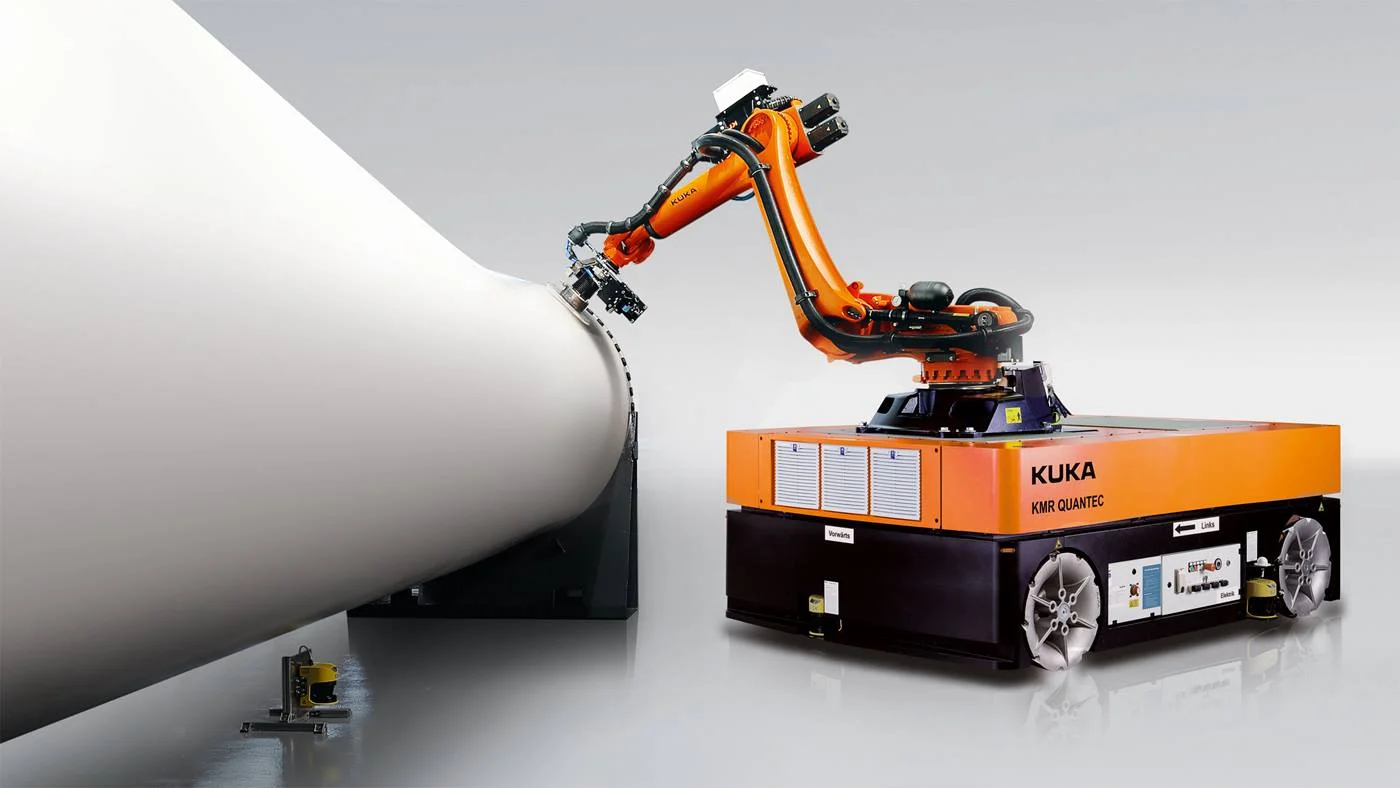
\includegraphics[width=0.4\linewidth]{Bilder/Grundlagen/industrie_mobiler_Roboter.png}}%
  \qquad
  \subfloat[][]{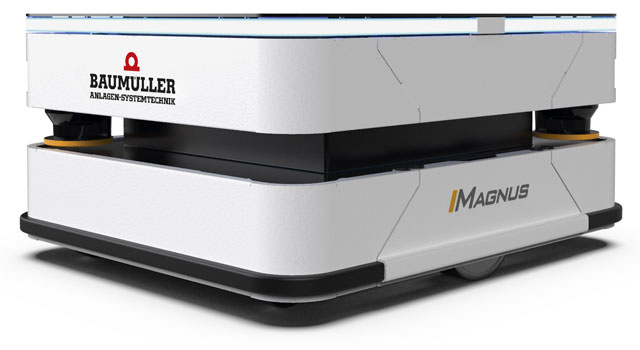
\includegraphics[width=0.4\linewidth]{Bilder/Grundlagen/bauMuellermagnus.jpg}}%
  \caption{Einsatz von mobilen Robotern in der Industrie (a) KMR QUANTEC \cite{KUKA_Roboter.2016} (b) Magnus der Firma Baumüller \cite{Baumueller.2021}}
  \label{fig:mobileRoboterIndustrie}
\end{figure}

\begin{figure}[]
  \centering
  \subfloat[][]{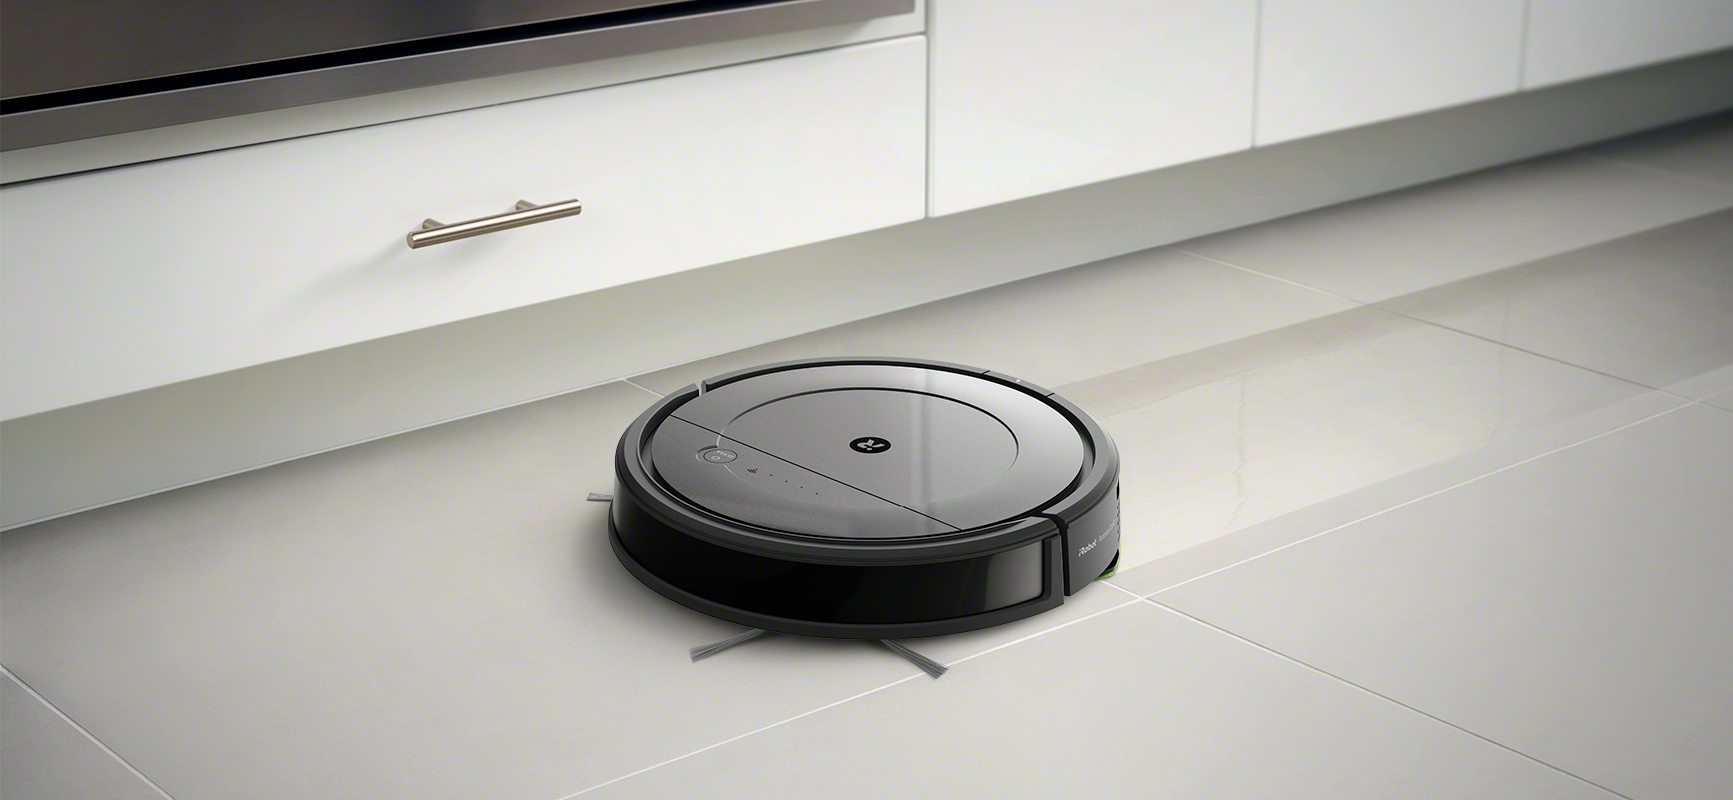
\includegraphics[width=0.4\linewidth]{Bilder/Grundlagen/IRobot_Wisch_Staubsauger.jpg}}%
  \qquad
  \subfloat[][]{\includegraphics[width=0.4\linewidth]{Bilder/Grundlagen/bosch_rasenmäroboter.jpg}}%
  \caption{Einsatz von mobilen Robotern in privaten Haushalten (a) Roomba Combo Saug- \& Wischroboter der Firma iRobot \cite{iRobot.2021} (b) Indego S+ 500 Roboter-Rasenmäher der Firma Bosch \cite{Boschdiy.2021}}
  \label{fig:mobileRoboterPrivaterHaushalte}
\end{figure}

Ein weiter Katastrophenfall ist die Corona Pandemie, die seit 2020 die ganze Welt in ihrem Bann hält. Die Pandemie hat viele Opfer gefordert, allein in Deutschland über 100.000, Stand 25.11.2021 \cite{tagesschau.25.11.2021}. Durch die leichte Übertragung hat sich das Virus zu einer Pandemie entwickelt. Die Corona Pandemie hat deutlich gemacht, das Keime und Viren auf Oberflächen an öffentlichen Orten und Arbeitsplätzen getötet werden müssen und dass es nicht nur ein Thema in Krankenhäusern ist. \cite{VDI_Corona_Roboter.2021} So konnte die autonome mobile Robotik sogar in der Pandemie an Wichtigkeit gewinnen. Es werden Serviceroboter entwickelt, die durch verschiedene Reinigungs- und Desinfektionsverfahren auf Oberflächen die Infektionsketten stoppen. Die Aufgabe der Desinfektionsroboter ist es zum Beispiel Türgriffe abzuwischen und im Anschluss über UV-Licht die Keime zu neutralisieren, sodass auch an schwer zugänglichen Stellen die Viren bzw. Keime getötet werden. Der mobile Roboter erkennt selbstständig durch Sensoren alle Objekte, die gereinigt werden müssen. \cite{VDI_Corona_Roboter.2021}
\newline
In dieser Arbeit soll eine Schnittstelle entwickelt werden, um die mobilen Roboter vereinfacht über Netzwerknachrichten zu bedienen. Dieses System soll als Grundlage dienen, um vereinfacht mobile Roboter in Bildungseinrichtungen als Lehrmaterial einzusetzen. Durch die standardisierten Schnittstellen können gezielt Benutzeroberflächen für unterschiedliche Anforderungen geschaffen werden, ohne die Implementierung am Roboter zu ändern.  


\section{Problemumfeld}
Die Abschlussarbeit entstand in Zusammenarbeit mit der Firma Kurt Hüttinger GmbH. Dabei war die Firma, während des Bearbeitungszeitraums, in einer wirtschaftlich schlechten Lage, da die Corona Pandemie das klein- und mittelständische Unternehmen belastete. Die Firma Hüttinger ist ein Unternehmen, das auf Messe- und Museumsbau spezialisiert ist. Da aber durch die Pandemie viele Ausstellungseinrichtungen geschlossen oder eingeschränkt sind, ist die Firma in eine wirtschaftliche Schieflage geraten, daher konnte der ursprüngliche mobile Roboter der Firma EduArt Robotik GmbH nicht bestellt werden. Die Arbeit wurde schließlich auf einen prototypischen Aufbau mithilfe vom Kobuki umgestellt. Infolgedessen wurde ein System angestrebt, das als Exponat in einem Museum bzw. einer Bildungseinrichtung ausgestellt werden kann. Die Abschlussarbeit soll eine offene Plattform bieten für die Bedienung von mobilen Robotern. Demnach können die Benutzeroberflächen für verschiedene Einrichtungen und Anforderungen entwickelt und geändert werden, ohne die roboternahe Implementierung zu ändern.  



\section{Zielsetzung} \label{sect:Zielsetzung}
In dieser Arbeit wird ein System ausgearbeitet, das in Bildungseinrichtungen zum Einsatz kommen könnte, um Kindern und Jugendlichen die Technik der allgegenwärtigen mobilen Roboter näher zu bringen. Dazu wird eine API entwickelt, die diese mobilen Roboter bedient und leichter zugänglich macht. So kann die Benutzeroberfläche zum Bedienen der mobilen Roboter offengehalten werden, da das API über Netzwerknachrichten bedient werden kann. Weiterhin werden in das API wichtige Funktionalitäten wie Hinderniserkennung implementiert. Dabei wird ein Kobuki Roboter für die experimentellen Tests verwendet.  
\chapter{Grundlagen - Stand der Technik}
In diesem Kapitel werden Grundlagen beschrieben, die relevant für das Verständnis dieser Arbeit sind. Die Arbeit über mobile Roboter ist ein aktuelles Thema und wird in vielen Arbeiten behandelt, deswegen entsteht hier eine Beschreibung, welche den Stand der heutigen Technik wiedergibt.

% \section{Stand der Technik}
\section{Roboter}
In der DIN ISO 10218-1:2021 wurde der Begriff Industrieroboter Roboter folgendermaßen erläutert: \glqq Industrieroboter Roboter [sind] automatisch gesteuerte(r), frei programmierbare(r) Mehrzweck-Manipulator(en) [...], der in drei oder mehr Achsen [...] programmierbar ist und zur Verwendung in Automatisierungsanwendungen [...] in einer Industrieumgebung [...] entweder an einem festen Ort oder fest an einer mobilen Plattform [...] angeordnet sein kann\glqq. \cite{DIN_ISO_Robotik.2021}\\

Der Begriff mobiler Roboter ist nicht eindeutig dargelegt, aber wenn man die einzelnen Begriffe für sich selbst definiert, bedeutet mobiler Roboter, das eine Maschine nicht fest, sondern frei in der Bewegung ist, was von ihrer aktuellen Umgebung abhängt. Die Aktion des mobilen Roboters ist erst zum Zeitpunkt der Ausführung bekannt, es läuft nicht nach einem bestimmten Ablaufplan ab, sondern entscheidet durch Sensorik die nächste Handlung. In dieser Arbeit nehmen wir an, das ein mobiler Roboter eine frei programmierte Maschine ist, die durch Umgebungseinflüsse interagiert. Dabei ist zum Zeitpunkt der Programmierung die Beeinflussung auf den Roboter unbekannt. \cite[S.1ff]{RobotikSichtInformatik.2012}\\

Die aktuellen Staubsaugroboter sind viel intelligenter als noch vor paar Jahren. Das Prinzip ist, frei in einem Raum zu saugen und wenn ein Hindernis leicht berührt wird, die Richtung zu ändern und weiterzumachen. Dieser Vorgang wird so lange wiederholt, bis verschiedene Aspekte erreicht sind, wie zum Beispiel eine vom Benutzer*in definierte Zeitangabe wird erreicht, Batterie Kapazität erreicht einen minimalen Level oder Saugbehälter ist überfüllt. Die aktuellen Roboter können auch Karten von den Räumen erstellen (siehe \autoref{fig:intelligenteFunktionenMobilerRoboter}[a]), die dann über eine Benutzeroberfläche vom Benutzer*in definiert werden, anschließend kann der Benutzer*in auf der Karte bestimmte Bereiche als unzugänglich markieren, wodurch die Roboter diesen Bereich nicht betreten. Deshalb kann der Roboter auch neue Hindernisse erkennen und die Verbraucher warnen mit einem Foto(siehe \autoref{fig:intelligenteFunktionenMobilerRoboter}[b]). Dazu wird eine weiterverbreitete Technik, das SLAM Verfahren, verwendet.

\begin{figure}[h]
  \centering
  \subfloat[][]{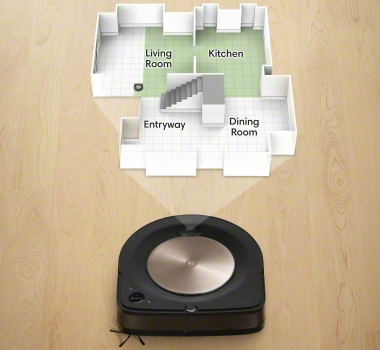
\includegraphics[width=0.4\linewidth]{Bilder/Grundlagen/iRobot_karten_erstellung.jpg}}%
  \qquad
  \subfloat[][]{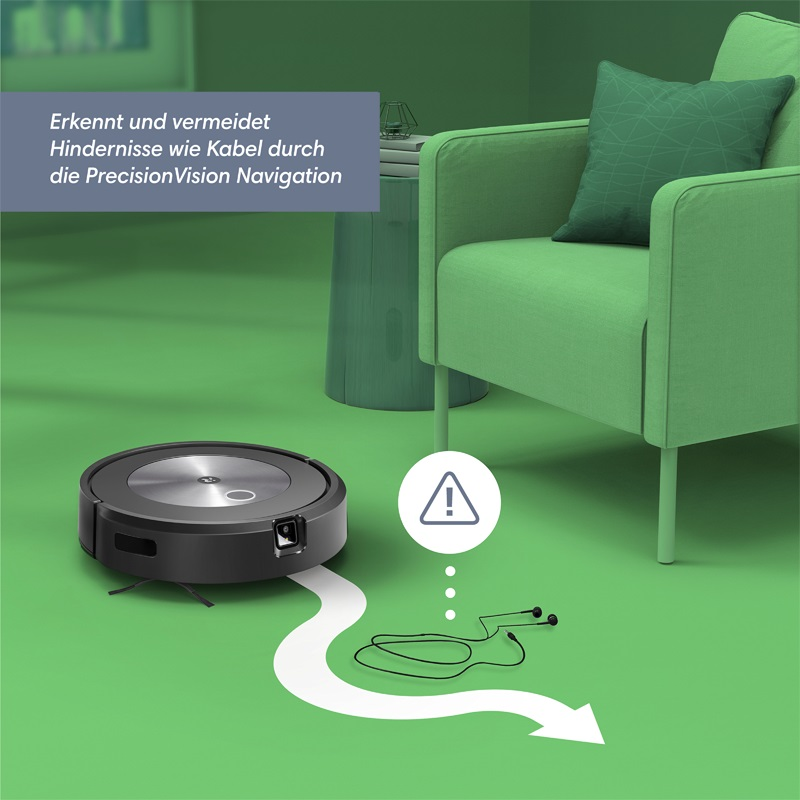
\includegraphics[width=0.4\linewidth]{Bilder/Grundlagen/iRobot_warnung_neue_hindernisse.jpg}}%
  \caption{Die intelligenten Funktionen eines Staubsaugroboters der Firma iRobot (a)\cite{iRootKarte.2021} (b)\cite{iRobotHindernissErkennung.2021}}
  \label{fig:intelligenteFunktionenMobilerRoboter}
\end{figure}



\section{Roboterkontrollarchitekturen}\label{subsec:Roboterkontrollarchitekturen}
Die Roboterkontrollarchitektur bezieht sich auf den Aufbau der Software für die Robotersteuerung. Dabei ist für eine gute Softwarearchitektur entscheidend, dass diese klare Strukturen hat, Daten- und Kontrollfluss gegliedert sind um die Wartbarkeit eines Programms zu verbessern. Die Kontrollarchitektur eines Roboters ist noch mal komplizierter, denn es ist ein System, das in einem geschlossenen Regelkreis läuft, das heißt Verarbeitung von Sensordaten in Echtzeit. Es kann dabei nicht auf einen standardisierten Daten- und Kontrollfluss gesetzt werden, schließlich sind die Datenarten jedes Roboters unterschiedlich. Dadurch kann festgehalten werden, dass es nicht die eine Architektur gibt, die besser als alle anderen ist. In dieser Arbeit wird das ROS (siehe \autoref{subsubsec:ROS}) verwendet, es ist einer der derzeit aktuellen und immer weiter verbreiteten Vertreter von Software-Tools und Kontrollstrukturen, was dabei hilft, einfach und robust ein System aufzubauen, ohne komplett eine Roboterkontrollsoftware zu programmieren. \cite[S.317ff]{RobotikSichtInformatik.2012}

% Die Roboterkontrollarchitektur bezieht sich auf den Aufbau der Software für die Robotersteuerung. Dabei ist für eine gute Softwarearchitektur entscheidend, dass diese klare Struktur hat, Daten- und Kontrollfluss gegliedert sind und die Wartbarkeit eines Programms zu verbessern also zusammengefasst wird auf die Kostensenkung bei der Softwareentwicklung über ihren Lebenszyklus gesetzt. Die Kontrollarchitektur eines Roboters ist noch mal komplizierte, denn sie sind ein System, das in einem geschlossenen Regelkreis laufen, das heißt Verarbeitung von Sensordaten in Echtzeit. Es kann dabei nicht auf einen standardisierten Daten- und Kontrollfluss gesetzt werden, schließlich sind die Datenarten jedes Roboters unterschiedlich. Dadurch kann festgehalten werden, dass es nicht die eine Architektur gibt, die besser als alle anderen ist. In dieser Arbeit wird das ROS (siehe \autoref{subsubsec:ROS}) verwendet, sie ist einer derzeit aktuellen und immer weiter verbreiten Vertreter von Software-Tools und Kontrollstrukturen was dabei hilft Einfache und Robuste ein System aufzubauen, ohne komplett eine Roboterkontrollsoftware zu programmieren. \cite[S.317ff]{RobotikSichtInformatik.2012} 


\subsection{ROS - Robot Operating System} \label{subsubsec:ROS}

\subsubsection{ROS Einführung}
Roboter Operating System oder kurz ROS ist ein quelloffener Software-Framework oder Meta-Betriebssystem für Roboter. Es stellt wie ein Betriebssystem Dienste zur Verfügung wie zum Beispiel Hardwareabstraktion, Gerätetreiber oder Paketmanagement. Dabei bietet ROS auch Softwaretools und Bibliotheken an. Das Framework setzt auf individuelle und entkoppelten Komponenten. \cite{ROSIntro.2021} Diese vielen Prozesse können auf unterschiedlichen Rechnern laufen und werden bei ROS zur Laufzeit mit Peer-to-Peer-Topologie vernetzt (siehe \autoref{fig:peerTopeerTopologie}).
\begin{figure}[H]
 \centering
 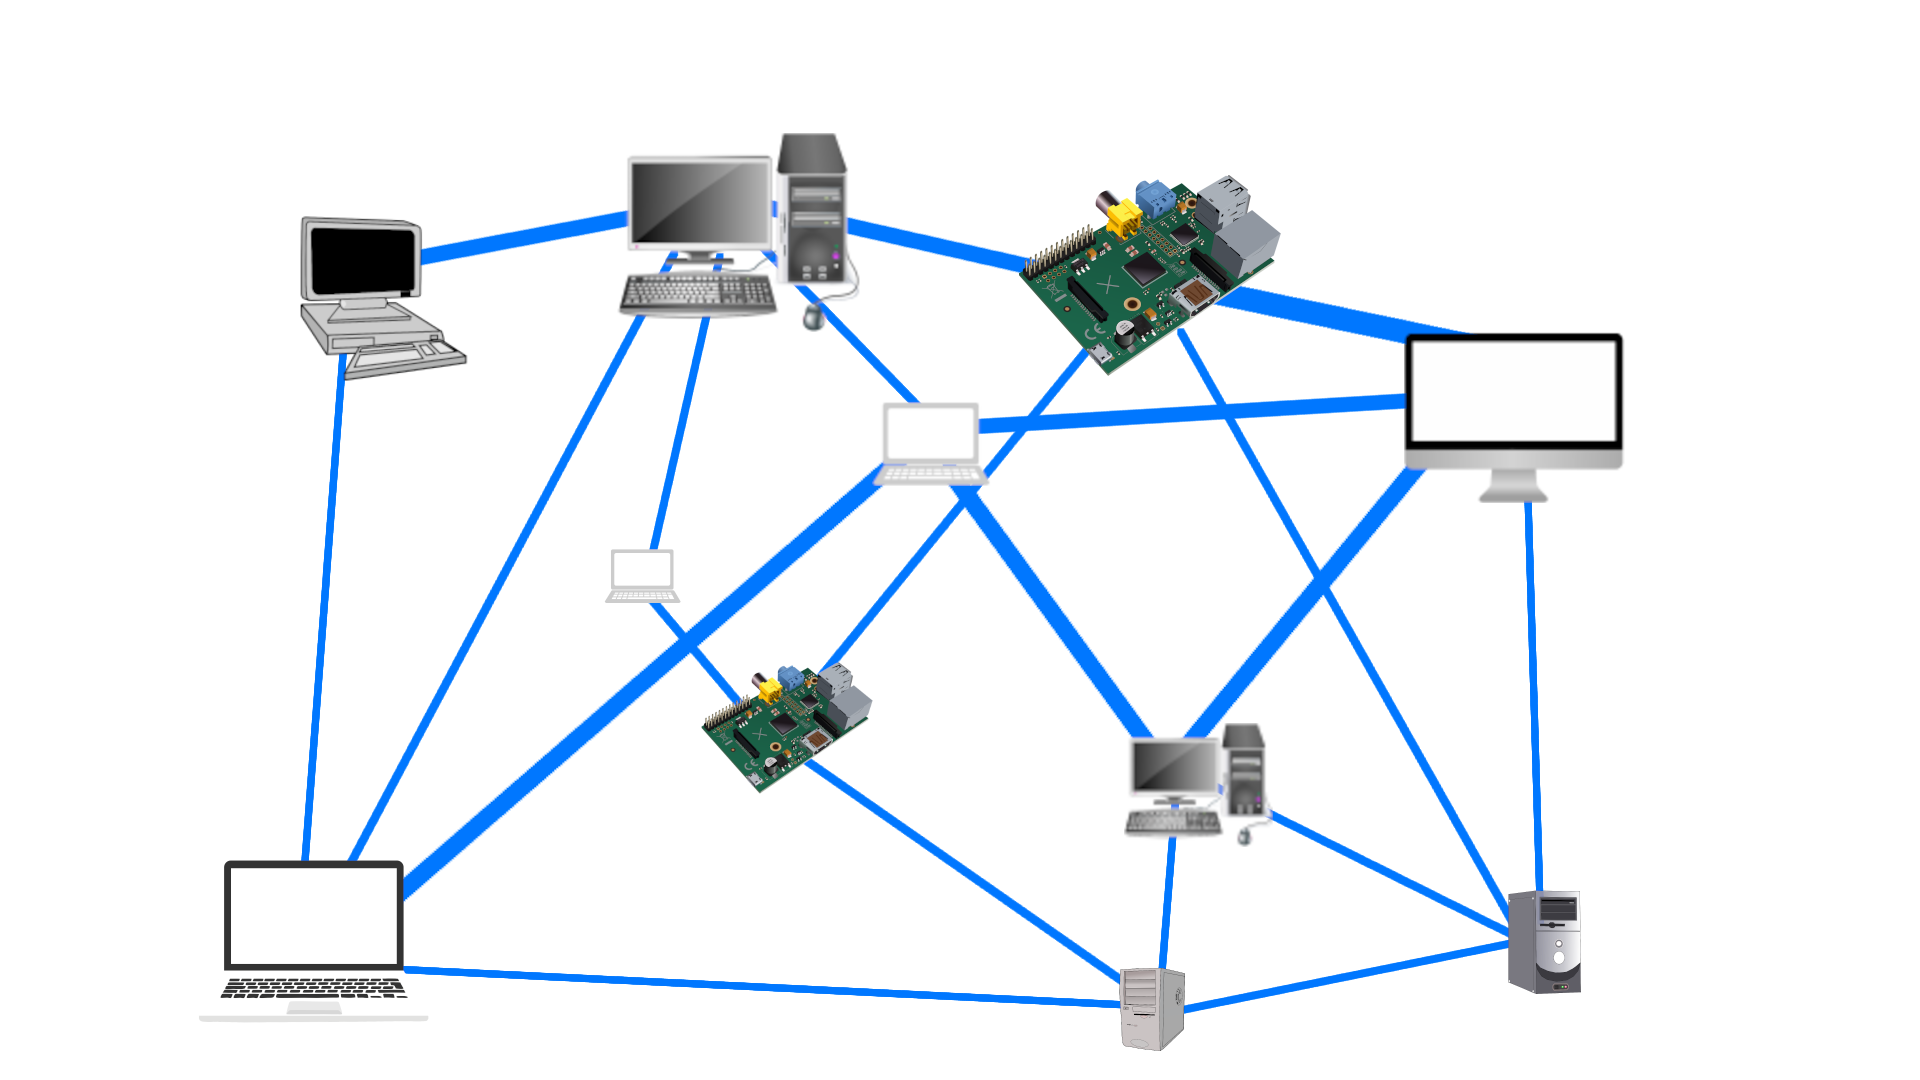
\includegraphics[width=0.7\linewidth]{Bilder/Grundlagen/peerTopeerTopologie.png}
 \caption{Netzstruktur einer Peer-to-Peer-Topologie}
 \label{fig:peerTopeerTopologie}
\end{figure}
Dadurch wird das System dezentralisiert und braucht keine zentralen Server. Durch diese Topologie sind alle Rechner gleichwertig, somit wird unnötiger Netzverkehr vermieden anders als bei Server-Client-Topologie (siehe \autoref{fig:serverClientTopologie}) da müssen alle Anfragen an den Server vermittelt werden. 

\begin{figure}[H]
 \centering
 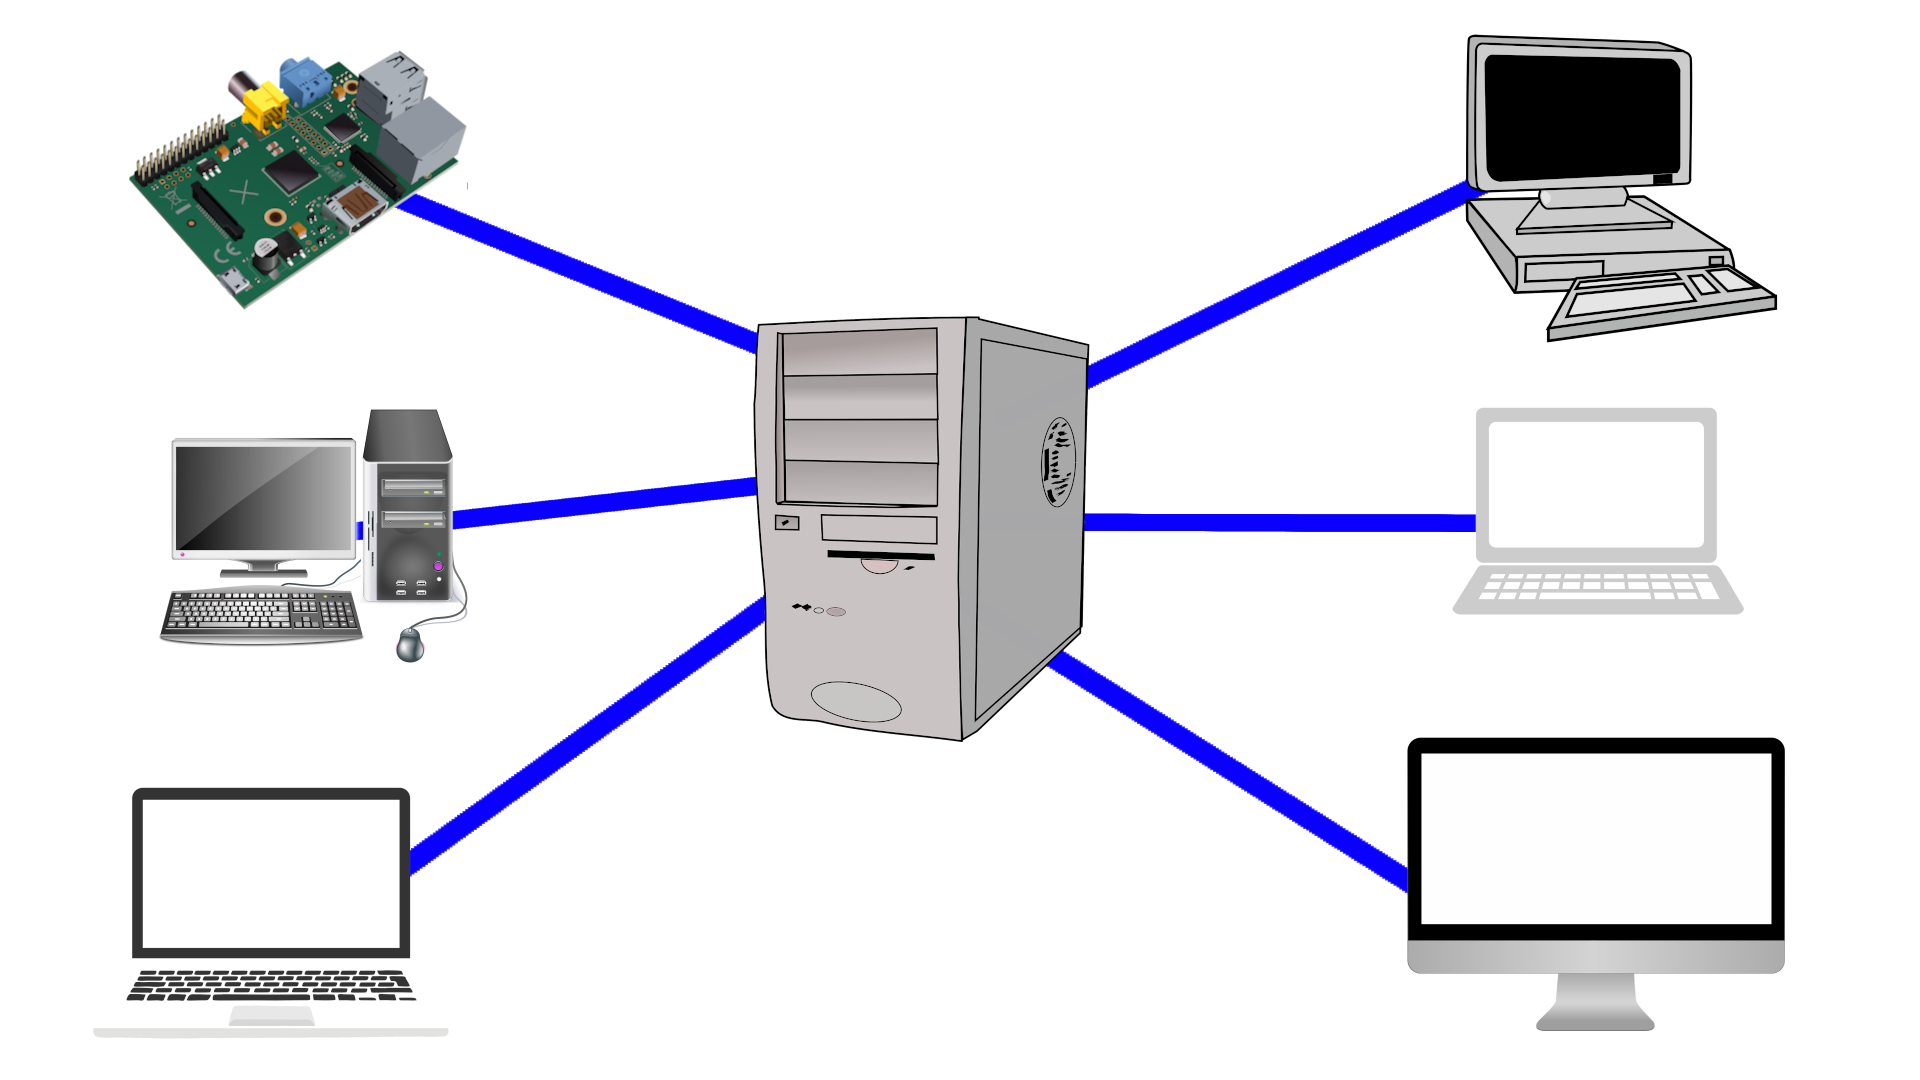
\includegraphics[width=0.7\linewidth]{Bilder/Grundlagen/serverClientTopoliogie.png}
 \caption{Netzstruktur einer Server-Client-Topologie}
 \label{fig:serverClientTopologie}
\end{figure}
Bei ROS gibt es lediglich einen Master, der für die Namensdienste, also Verzeichnisse der Prozesse zuständig ist, damit die Rechner sich gegenseitig finden. \cite{RobotikSichtInformatik.2012}
Aus den Zielen des ROS haben sich die folgende wichtigen Punkte deutlich gemacht.\\ 
\textit{Mehrsprachig}, am Anfang wurden nur C++, Python, Octave und LISP unterstützt und jetzt werden alle wichtigen Sprachen unterstützt. Dieses Ziel soll dazu dienen, dass es keine Beschränkung für die Programmierer gibt, denn die Präferenz einzelner Entwickler sind unterschiedliche Programmiersprachen.\\
\textit{Schlank}, denn ROS ist nur ein Framework und dienst nur dazu, Daten in das Programm zu führen und Resultate abzufangen und zu übertragen. Dementsprechend setzt ROS voraus, dass alle Treiber und Algorithmen keine Abhängigkeit haben und eigenständig implementiert werden.\\
\textit{Werkzeugbasiert}, ROS bietet viele verscheiden Tools an, die verwendet werden können, um z. B. Tests zu vereinfachen mit rostest, Verzeichniswechsel zu ROS Paketen mit roscd oder zur Visualisierung der Netztopologie mit rqt\_graph. Diese ganzen Softwaretools vereinfachen und helfen bei der Entwicklung. \cite[S.326ff]{RobotikSichtInformatik.2012}

\subsubsection{ROS Konzept}

\paragraph{ROS-Datensystem-Ebene}\mbox{}\\
Die ROS Architektur hat drei Entwicklungsschichten, dazu zählt als erstes das ROS Datensystem. Die Datensystemebene umfasst grundsätzlich die ROS-Ressourcen, die wichtigsten werden im Folgenden näher beschrieben. \\

Als Erstes sind Pakete zu erwähnen, sie bilden die Grundeinheit für die Software in ROS. Sie beinhalten ROS-Prozesse wie Nodes, Bibliotheken, Konfigurationsdaten oder alles andere, was sinngemäß zusammengehört. Pakete sind die elementarste Einheit, die erzeugt und veröffentlicht werden können. \\
Metapakete sind verwandte Pakete, die in eine Gruppe zusammengefasst werden. Dabei kann beispielhaft das Paket vom Kobuki erwähnt werden, welches verschiedene Funktionalitäten in einem Metapaket zusammenfasst, wie Kobuki automatische andocken, Kobuki sichere Kontrollfahrt oder das Paket für normale Kobuki Fahrt. Diese funktionalen Pakete werden dann in einem Metapaket gesammelt. \\
Paket-Manifests, die Datei „package.xml“ liefert Metainformation über das Paket wie z. B. Name, Version, Lizenzinformation, Abhängigkeiten und andere Metadaten. \cite{ROSKonzept.2021, RoboterMitRos.2020} \\

\paragraph{ROS-Berechnungsgraphen-Ebene} \mbox{} \label{hl:ROS_Berechnungs_Ebene}\\
Als weitere Ebene in der ROS-Architektur ist die ROS-Berechnungsgraphen-Ebene zu erwähnen. Sie ist ein Peer-to-Peer Netzwerk aus Ros-Prozessen. Dabei sind die grundlegenden Konzepte der Ebene, \textit{Nodes}, \textit{Master}, \textit{Parameter Server}, \textit{Messages}, \textit{Services}, \textit{Topics} und \textit{Bags}, die allesamt unterschiedliche Daten bereitstellen. Im Folgenden werden die wesentlichsten Konzepte der Ebene näher erläutert. \\

Nodes (Knoten) sind die Prozesse, die Aufgaben durchführen. Die ROS Architektur ist modular aufgebaut, so kann eine Roboterkontrollarchitektur aus mehreren Knoten bestehen. Die einzelnen Knoten können verschiedene Berechnungen steuern wie Laserentfernungsmessung, Lokalisierung, Manövrieren oder Pfadfindung. Nodes können mithilfe ROS-Bibliotheken implementiert werden und können auch untereinander kommunizieren, wenn sie parallel laufen. \\ 
Master stellt die Namensregistrierung und Namenssuche für die ROS-Berechnungsgraphen-Ebene zur Verfügung. Der Master ist ein zentraler Bestandteil, ohne ihn könnte kein Kommunikationsaustausch stattfinden. ROS arbeitet mit TCPROS das aber standardmäßig TCP/IP-Socket verwendet, wobei es XMLRPC-Nachrichten sind, die mit TCP verschickt werden. Der Standard-TCP-Port läuft auf 11311 und wartet auf Nachrichten, wobei die genaue Netzwerkadresse eingestellt werden kann, aber standardmäßig auf localhost, also auf die Netzwerkadresse des laufenden Rechners eingestellt ist. Das ROS über Netzwerknachrichten arbeitet, hat den Vorteil, dass leicht auf und mit entfernten Rechner kohäriert werden kann. Der ROS-Master kann mit \textit{roscore} oder \textit{roslaunch} gestartet werden, unterdessen müssen sich alle Prozesse am Anfang beim Master registrieren (siehe \autoref{fig:Roskommunikationsprinzip}) um die Bekanntmachung der Knoten mitzuteilen ob publiziert oder abonniert wird.

\begin{figure}[H]
 \centering
 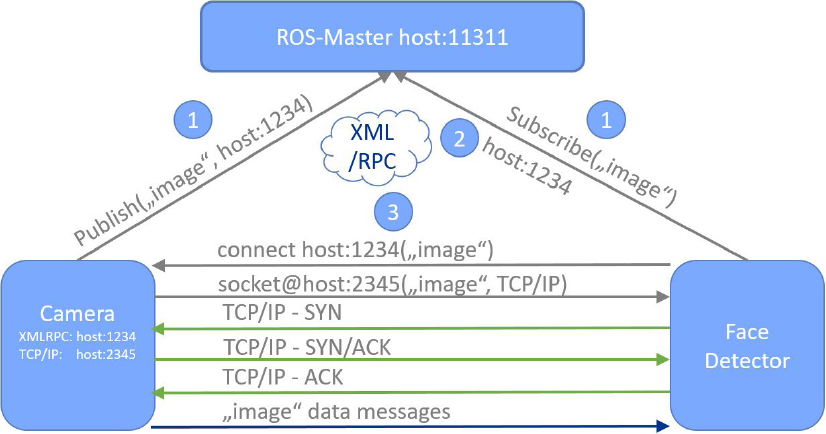
\includegraphics[width=\linewidth]{Bilder/Grundlagen/ROS-Kommunikation.png}
 \caption{ROS-Kommunikationsmodes \cite{RoboterMitRos.2020}}
 \label{fig:Roskommunikationsprinzip}
\end{figure}


Die \autoref{fig:Roskommunikationsprinzip} zeigt deutlich, dass der Master nur als ein Vermittler dient und nur die Verbindung der Nodes veranlasst, ähnlich wie ein DNS-Server. Die Daten werden nur noch zwischen den Nodes verschickt, ohne Bezug zum Master. So wird eine Stabilität des ganzen Systems garantiert, denn wenn ein Prozess ausfällt, hat es keinen Einfluss auf die anderen Prozesse oder Master. So kann auch bei einem bestehenden Datenfluss der Ausfall durch Wartezeit überwunden werden ohne dass alle Prozesse aufgehalten werden. \\


Der Parameter-Server ermöglicht, die Konfiguration von Daten nach Schlüssel an einem zentralen Ort zu speichern, aber ausgelagert vom Programmcode. Der Parameter Server läuft innerhalb des ROS-Master und ermöglich so Quellcodeabschnitte variabel zu halten. Durch Verwendung des Parameter-Server müssen bei Änderungen nicht die Nodes neu kompiliert werden.\\ 
Messages sind Datenstrukturen, die zur Kommunikation von Knoten miteinander verwendet werden. Diese Nachrichten werden in einer \textit{.msg}-Datei definiert. Es werden einfache Datentypen und mehrdimensionale Arrays unterstützt. Nachrichten können beliebig verschachtelt werden so ähnlich wie bei \textit{C-structs}. \\
Topics sind Namen für Nachrichten, die zur Identifikation der Nachricht dient. ROS arbeitet wie zuvor erwähnt mit Publish/Subscribe-Semantik so kann ein Knoten eine Nachricht zu einem bestimmten Topic veröffentlichen (Publish) und von einem oder mehren Knoten kann dieser Topic abonniert (Subscribe) werden (siehe \autoref{fig:topicModell}), um die Nachricht zu erhalten. Dadurch müssen die Knoten sich nicht kennen, vereinfacht gesagt kann es als ein BUS-System angenommen werden. Jeder kann sich am BUS beteiligen, um Nachrichten zu verschicken oder zu empfangen.\\

\begin{figure}[H]
  \centering
  \subfloat[][]{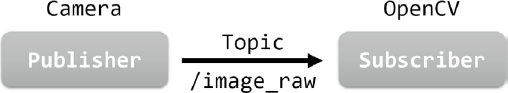
\includegraphics[width=0.4\linewidth]{Bilder/Grundlagen/topic.png}}%
  \qquad
  \subfloat[][]{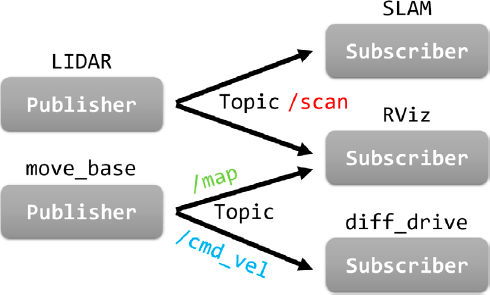
\includegraphics[width=0.4\linewidth]{Bilder/Grundlagen/moreTopics.png}}%
  \caption{ROS-Topic Modell (a) Einfacher Publischer und Subscriber Modell (b) Multiple Publischer und Subscriber Modell \cite{RoboterMitRos.2020}}
  \label{fig:topicModell}
\end{figure}

Services ist ein Kommunikationsmodell, das bidirektional ist, also ein Datenfluss in beide Richtungen. Dabei arbeiten Services als Anfrage-Antwort-Modell und werden ähnlich wie Messages in \textit{.srv}-Datei definiert. \\
Bags sind eine Art Format zur Speicherung und Wiedergabe von ROS-Nachrichten. Dies kann dazu verwendet werden, um Sensordaten, die schwer zu sammeln sind, zu speichern, um dies bei der Entwicklung abzuspielen. \cite{ROSKonzept.2021, RoboterMitRos.2020}

\paragraph{ROS-Community-Ebene} \mbox{}\\
Die dritte und letzte Schicht ist die Community Schicht, sie dient zum Austausch von Software und Wissen rund um ROS. Dabei gibt es verschiedene Plattformen und Lösungen, die weltweit zum Austausch zur Verfügung gestellt werden. Dazu zählt z. B. ROS-Distribution, die eine versionierte konsistente Softwaresammlung ist, Repositories, sie erweitern und ergänzen die Softwarepakete von ROS mit Softwarelösungen des weltweiten ROS-Netzwerks und Institutionen. Die ROS-Wiki Webseiten, sie sind die Hauptwissensvermittler für Dokumentationen und Tutorials. Das Bug-Ticket-System ist eine Zentrale Verwaltungsstelle, der Fehler gemeldet werden und vom ROS-Netzwerk bearbeitet werden. \cite{ROSKonzept.2021}

\section{Sensorik}\label{subsec:Sensorik}

Die Handlung eines mobilen Roboters in der Umgebung wird mit Sensoren bestimmt. Die Sensorik widerspiegeln die Sinne eines Menschen (siehe \autoref{tab:ParalellenzwsichenMenschundSensorik}) für einen Roboter. Menschen können mit dem Auge die Umgebung wahrnehmen, wie Entfernungen abschätzen, Helligkeit, Objekte und Hindernisse erkennen. Dabei können wir Menschen es auch nicht alles ab dem Zeitpunkt der Geburt, sondern es ist eine langwierige Lernphase, die unser ganzes Leben andauert. Schließlich können wir Objekte erkennen, die wir auch vorher kennengelernt und im Gehirn abgespeichert haben. Ein weiteres Beispiel ist die Entfernungsabschätzung, die wir erst durch Lernen der Messeinheiten erlernt haben. So wissen wir, das auf der Autobahn die Leitpfosten mit 50 Meter Abstand aufgestellt sind und können daher den Abstand zum vorausfahrenden Fahrzeug einschätzen. Ebenso kann ein Roboter auch die Entfernung schätzen, indem er auf seine spezifischen Sensoren zugreift und die physikalischen Größen misst.
\begin{table}[H]
\begin{tabular}{|l|l|l|l|l|}
\hline
\textbf{Mensch}         & \textbf{Sinn}          & \textbf{Organ}        & \textbf{Sensorik} & \textbf{Erfassung von} \\ \hline\hline
Hören                   & Gehör                  & Ohr                   & Mikrofon          & Schall                 \\ \hline
\multirow{2}{*}{Sehen}  & \multirow{2}{*}{Licht} & \multirow{2}{*}{Auge} & Fotozelle         & Licht, Konturen        \\ \cline{4-5} 
                        &                        &                       & Kamera            & Szenen                 \\ \hline
\multirow{4}{*}{Fühlen} & Temperatur             & Haut                  & Thermometer       & Wärme                  \\ \cline{2-5} 
                        & Schwere                & Muskel                & Waage             & Masse                  \\ \cline{2-5} 
                        & Kraft                  &                       & Dehnmessstreifen  & Kraft, Drehmoment      \\ \cline{2-5} 
                        & Tastsinn               & Nerven                & Fühler, Schalter  & Form, Lage             \\ \hline
Riechen                 & Geruch                 & Nase                  & Rauchmelder       & Rauch, Gasen           \\ \hline
Schmecken               & Geschmack              & Zunge/Gaumen          & Künstliche Zunge  & Inhaltsstoffen         \\ \hline
\end{tabular}
\caption{Parallelen zwischen Mensch und Sensorik \cite{SensorenAutomation.2014}}
\label{tab:ParalellenzwsichenMenschundSensorik}
\end{table}
Die Sensorik misst physikalische Eigenschaften und wandelt es in ein elektrisches Signal um. Sensoren können in zwei Gruppen unterteilt werden, die interne oder externe Zustände erfassen. Beschaffenheiten, die im Inneren erfasst werden, sind z. B. Radgeschwindigkeit oder Radbeschleunigung, diese werden propriozeptive Sensorik genannt. Im Gegensatz dazu werden Zustände, die extern also umgebungsabhängig erfasst werden wie z. B. Ultraschallsensoren oder Kameras exterozeptive Sensorik genannt. In diesem Kapitel werden die Sensoren näher beschrieben, die für diese Arbeit verwendet wurden. 

\subsection{Entfernungsmessungen}

Damit ein mobiler Roboter die Umgebung wahrnehmen kann, muss er seine Distanz zu Objekten messen. Dabei gibt es drei Methoden, um mit der Sensorik die Entfernung zu messen. Diese drei Arten werden im folgend kurz näher erläutert. 
\subsubsection{Laufzeitmessung}\label{subsubsec:Laufzeitmessung}
Diese Art von Messung ist eine zeitabhängige und somit hängt die Genauigkeit von der Zeit ab. Dabei sendet die Sensorik Signale aus und misst die Zeit, bis ein Echo vom ausgesendeten Signal empfangen wird. Durch die gemessene Zeit kann die Strecke berechnet werden mit der einfachen Geschwindigkeitsformel (siehe \autoref{strecke}). 

\begin{align}
\centering
s &= v \cdot t \label{strecke}
\end{align}
Solche Sensoren sind angewiesen vom externen Umfeld also kann es der Gruppe von exterozeptiver Sensorik zugeordnet werden. Die Formel \autoref{entfernung} hat zwei Unbekannte, t die Zeit, die das Signal für die Strecke Hin und Zurück braucht, diese wird gemessen. Die zweite Unbekannte ist die Geschwindigkeit v, diese ist durch die physikalischen Eigenschaften vorgegeben wie z. B. Geschwindigkeit von Schall bei Zimmertemperatur, diese ist 343 m/s oder z. B. die Lichtgeschwindigkeit ist 299792458 m/s. So kann die Entfernung gemessen und geschätzt werden. 

\begin{figure}[H]
 \centering
 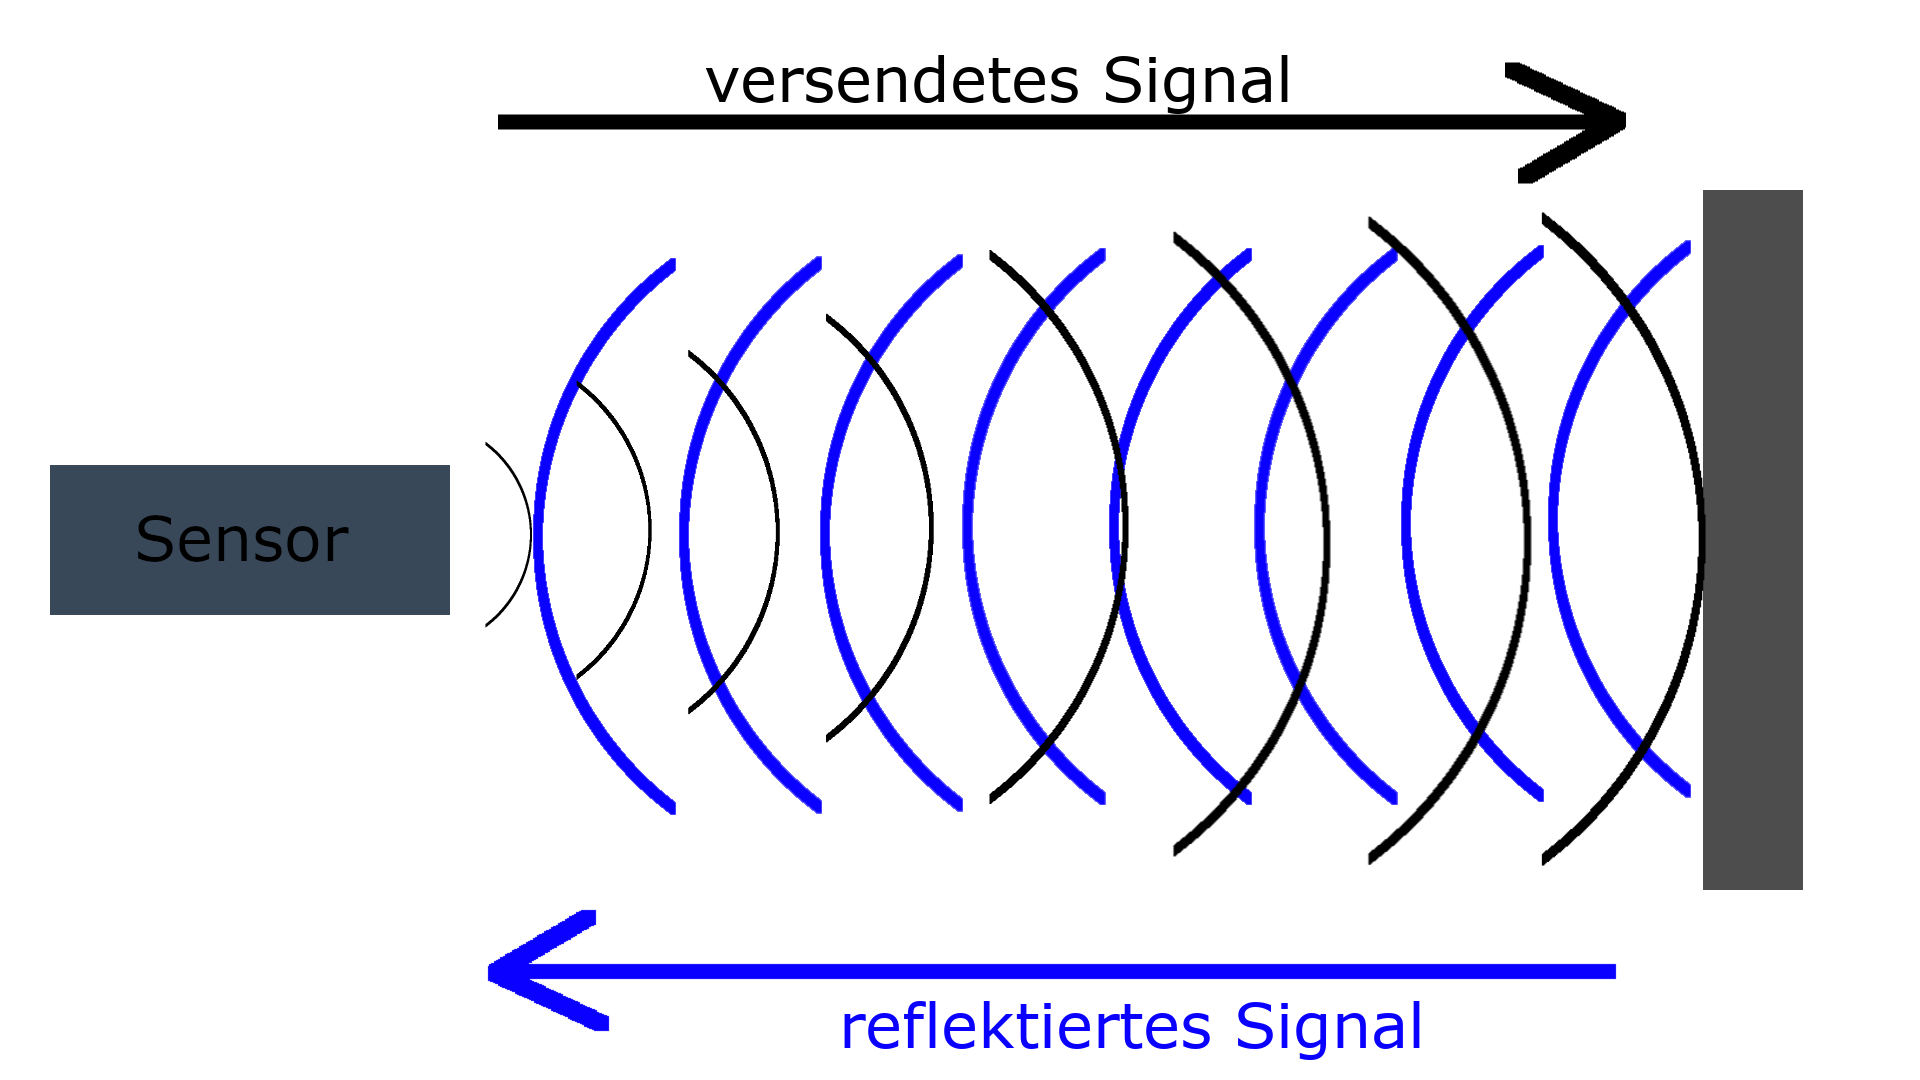
\includegraphics[width=\linewidth]{Bilder/Grundlagen/LaufzeitmessungGrafik.png}
 \caption{Grafische Darstellung von Laufzeitmesssystems}
 \label{fig:laufzeitmessungsgrafik}
\end{figure}

\begin{align}
\centering
D &= v \cdot \dfrac{t}{2} \label{entfernung}
\end{align}
Dabei ist noch zu beachten, dass die Zeit, die gemessen wurde für den Hin- und Rückweg ist (siehe \autoref{fig:laufzeitmessungsgrafik}), die Entfernung zu Objekten ergibt sich somit aus der Hälfte der gemessenen Zeit (siehe \autoref{entfernung}).\cite[S.36f]{RobotikSichtInformatik.2012}

\subsubsection{Phasendiffernezmessung}
Diese Messmethode ist eine ähnliche Art wie die Laufzeitmessung (siehe \autoref{subsubsec:Laufzeitmessung}) nur das hier die Phasenverschiebung von einer Welle gemessen wird. Die ermittelte Phasenverschiebung $\Delta\varphi$ ist proportional zur zurückgelegten Strecke D des Signals (siehe \autoref{entfernungPhasendifferenz}). 
\begin{align}
\centering
D &= \dfrac{\Delta\varphi \cdot \lambda }{4\pi} \label{entfernungPhasendifferenz} = \dfrac{\Delta\varphi \cdot v }{4\pi \cdot f}
\end{align}
Die Phasenverschiebung ist nur ein relatives Verhältnis des Signals zur Wellenlänge, deswegen werden verschiedene Signale modelliert, um mit hochfrequentem Anteil große Auflösung zu erreichen und mit niederfrequentem Anteil werden größere Entfernungen bestimmt. \cite[S.37f]{RobotikSichtInformatik.2012}

\subsubsection{Triangulation}\label{subsubsec:Triangulation}
Bei der Triangulationsmessung wird ein Signal ausgesendet und am Empfänger wird die Auslenkung x zum Abstand b gemessen. Durch den Strahlensatz kann dann die Distanz errechnet werden (siehe \autoref{entfernungTriangulation}). \begin{align}
\centering
D &= f\cdot\dfrac{b}{x} \label{entfernungTriangulation}
\end{align}
Die folgende \autoref{fig:Triangulationsprinzip} macht deutlich, dass der Bereich nahe am Sensor durch kleine Brennweite f und Parallaxe b möglich ist, aber anders ist es, wenn die Messung weitere Distanzen auflösen soll, denn dann muss die Brennweite f und Parallaxe b möglichst groß sein. Die Sensoren, die über diesen Messverfahren arbeiten, haben einen Totbereich, der keine Messwerte liefert.\cite[S.38f]{RobotikSichtInformatik.2012}
\begin{figure}[H]
 \centering
 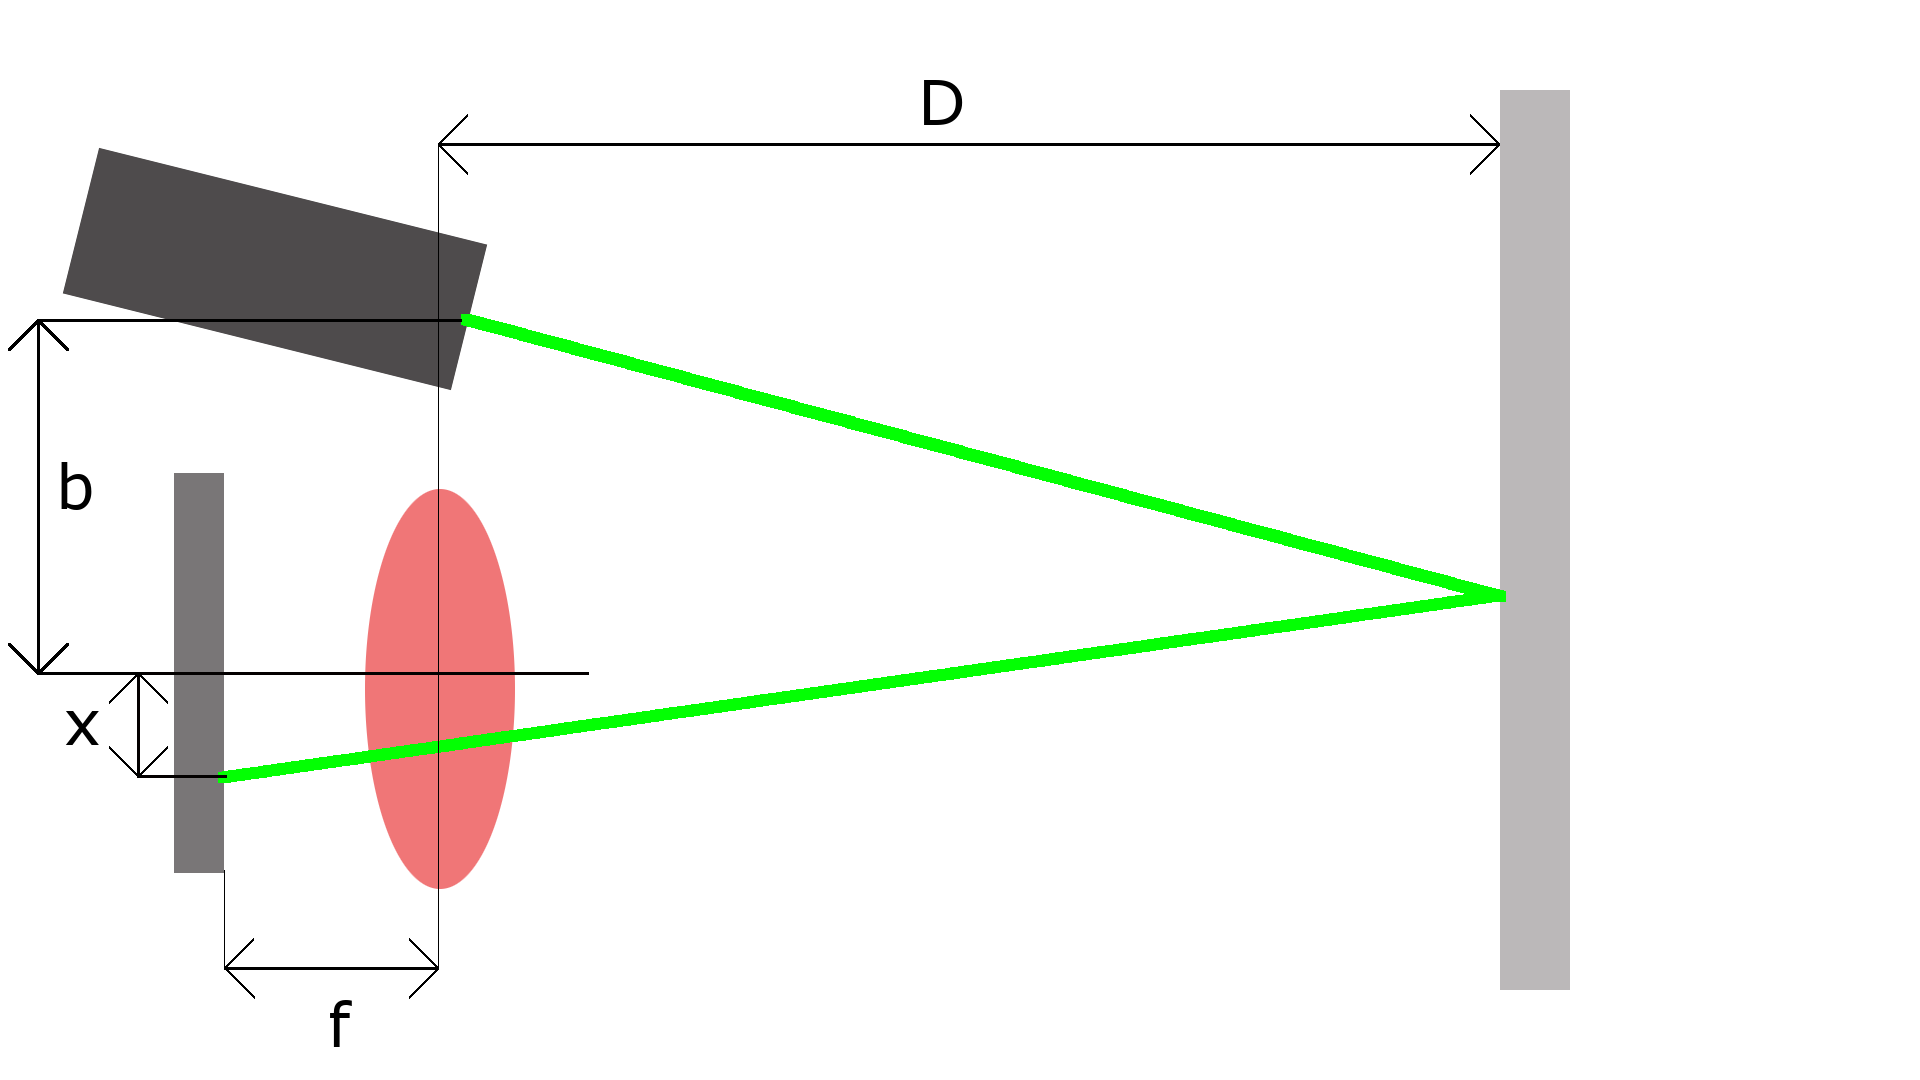
\includegraphics[width=0.98\linewidth]{Bilder/Grundlagen/Triangulationsprinzip.png}
 \caption{Triangulationsprinzip zur Distanzmessung}
 \label{fig:Triangulationsprinzip}
\end{figure}


\subsubsection{Ultraschallsensor}
Dieser Typ von Sensorik zur Entfernungsmessung arbeitet auf der Basis von Laufzeitmessung (siehe \autoref{subsubsec:Laufzeitmessung}). Ultraschallsensoren haben einen Öffnungswinkel. Außerhalb dieses Winkels und im Blindbereich nahe am Sensor kann keine Messung erfolgen. In dieser Arbeit wurden die Ultraschallsensoren HC-SR04 verwendet, die im Embedded Umfeld ihre Verwendung finden. 
Der Sensor wird mit einem Trigger Impuls angesteuert, anschließend sendet der Sensor ein Ultraschallsignal. Nachdem das Signal beendet wurde, wird der Echo Ausgang vom Sensor auf Logikpegel High gezogen und die Zeitmessung beginnt. Die Messung wird beendet, wenn ein Echo Signal am Empfänger ankommt, somit wird dann das Echo Ausgang auf Logikpegel Low gesetzt. Das Ultraschallsignal breitet sich mit Schallgeschwindigkeit in der Luft aus. 

\subsubsection{LiDAR}
Eine weitere Art von Sensorik, die in dieser Arbeit verwendet wird, ist ein LiDAR Scanner. Bei LiDAR Sensoren werden die zuvor beschriebenen Methoden verwendet, je nach Hersteller und Modell. Die in dieser Arbeit verwendeten RPLiDAR A1 der Firma Slamtec messen mit der Triangulationsmethode (siehe \autoref{subsubsec:Triangulation}). Der Scanbereich dieses 2D-Senors beträgt $360^\circ$ und hat eine Scanreichweite von $0,15\, m$ und $12\, m$. Solche Sensoren liefern nur die Distanz die gemessen wurde und über die Nummer oder Index der Liste aller Werte kann der Winkel bestimmt werden. Das bedeutet das es Polarkoordinaten sind, die als Messdaten vorliegen. Diese können aber ins kartesische Koordinatensystem umgerechnet werden (siehe \autoref{umrechnungPolarKartesischeKoordinaten}), so kann auch eine Karte des Raumes erstellt werden. 
\begin{align}\label{umrechnungPolarKartesischeKoordinaten}
\centering
\begin{split}
x &= r \cdot \cos(\varphi) \\
y &= r \cdot \sin(\varphi)
\end{split}
\end{align}

\subsection{Odometrie}
Das Odometrie Verfahren ist für die Positionsbestimmung relevant. Dabei wird über Sensoren am Rad des Roboters die Eigenbewegung gemessen, die dann durch eine vektorielle Addition verrechnet wird. Dabei werden oft für die Drehwinkelmessung Sensoren wie Impulsgeber oder Inkrementalgeber verwendet. 
\begin{figure}[H]
 \centering
 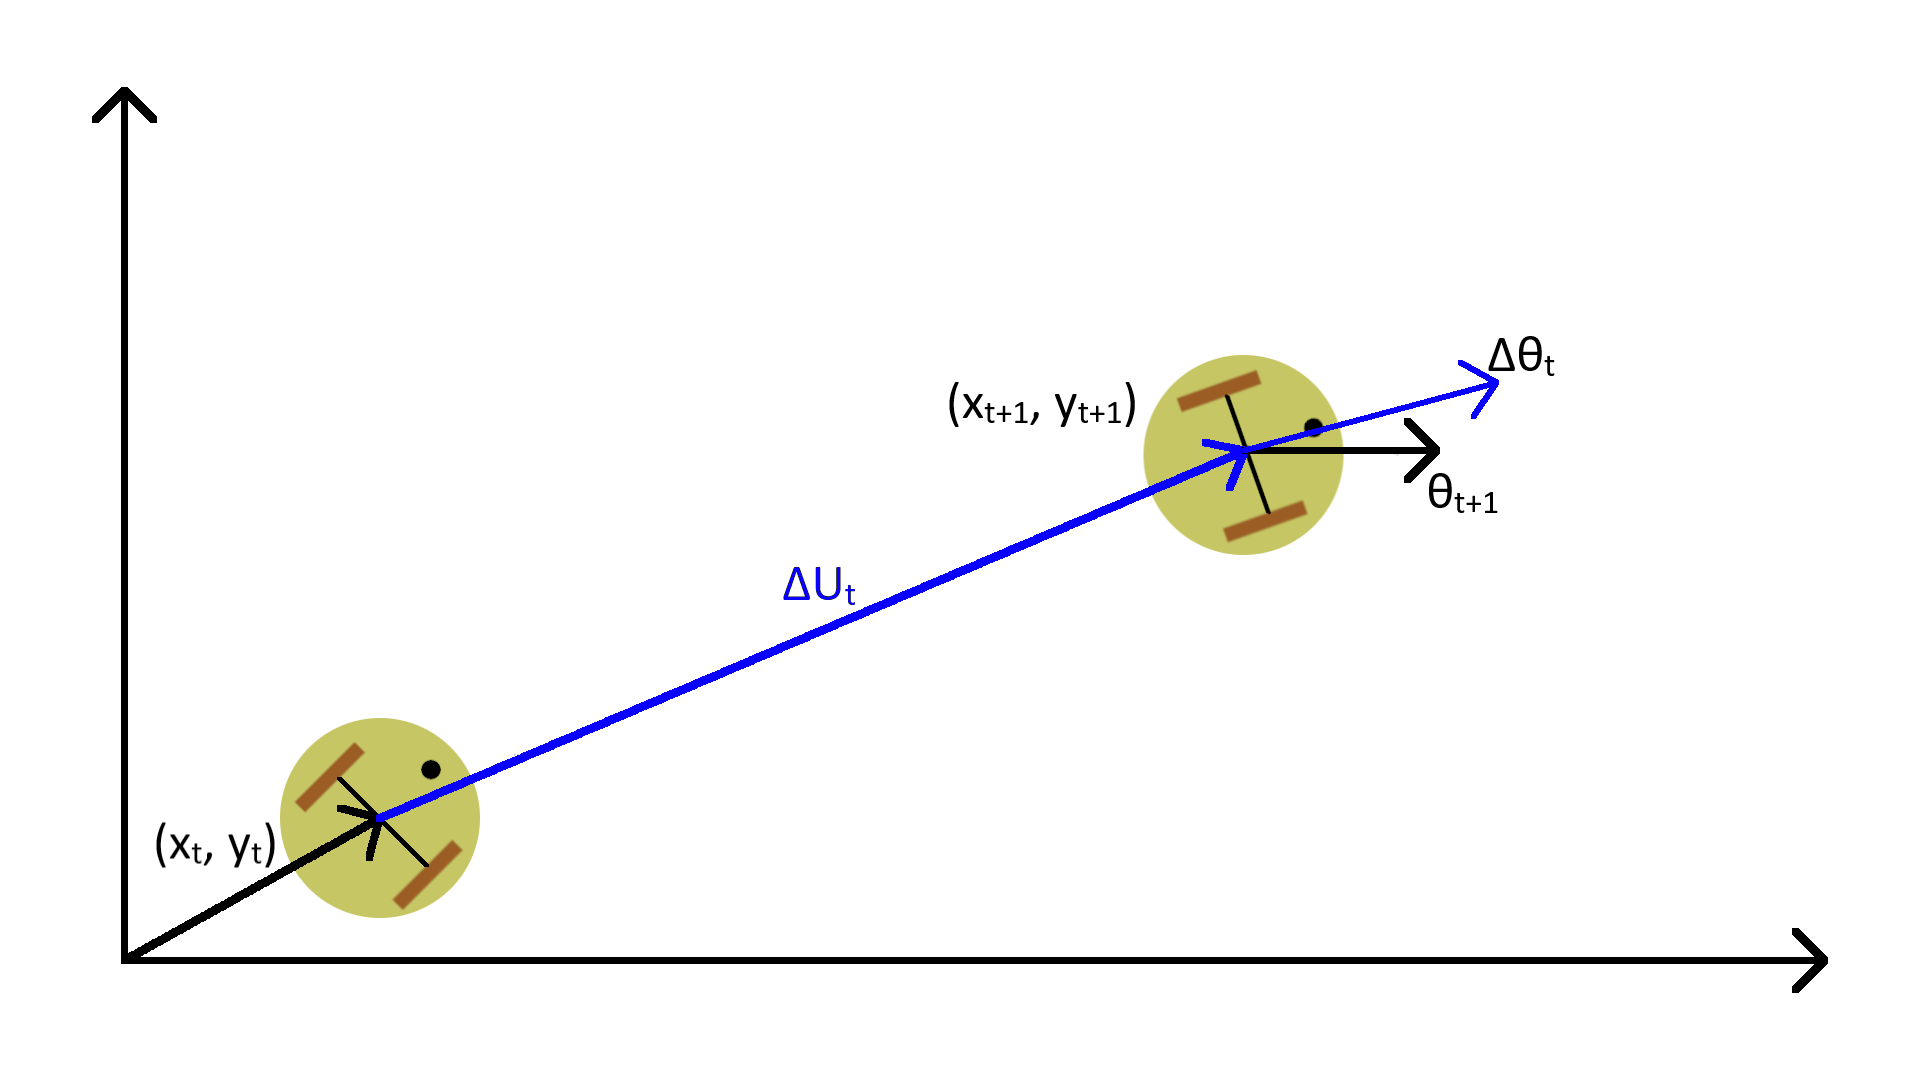
\includegraphics[width=0.9\linewidth]{Bilder/Grundlagen/odometrie.png}
 \caption{Bewegung eines mobilen Roboters}
 \label{fig:odometrieBewegung}
\end{figure}
Die folgenden diskreten Zustandsgleichungen beschreiben die Bewegung für die  \autoref{fig:odometrieBewegung}:
\begin{align}\label{odometrieZustandsgleichung}
\centering
x_{t+1} &= x_{t} + \Delta U_{t} \cdot \cos(\theta_{t}) \\
y_{t+1} &= y_{t} + \Delta U_{t} \cdot \sin(\theta_{t}) \\
\theta_{t+1} &= \theta_{t} + \Delta\theta_{t}
\end{align}

Dieses Verfahren hat oft einen Drift, der zustande kommt durch Schlupf an den Rädern oder Kollisionen mit Steinen. Die fehlerhaften Messungen werden jedoch weiter drauf addiert, was dazu führt, dass der Fehler immer größer wird. Um solche Fehler zu kompensieren, muss die Odometrie mit anderen Sensoren kombiniert werden.\cite[S.171ff]{SensorenAutomation.2014}

\subsection{Gyroskope} \label{subsubsec:gyroskope}
Diese Art von Sensoren erfassen Drehbeschleunigungen bezüglich des Roll-, Nick- und Gierwinkels. In der natürlichen Form ist es ein schnell drehender Kreisel, der beweglich gelagert ist (siehe \autoref{fig:gyroscope}). Da es ein geschlossenes System ist, führt das dazu, das alle Impulse konstant bleiben. Versucht eine äußere Kraft das Gyroskop zu beeinflussen, so reagiert er drauf und kippt sich senkrecht zur angreifenden Kraft. Die dabei erzeugten Drehmomente werden erfasst und als Sensormessung ausgegeben.
\begin{figure}[H]
 \centering
 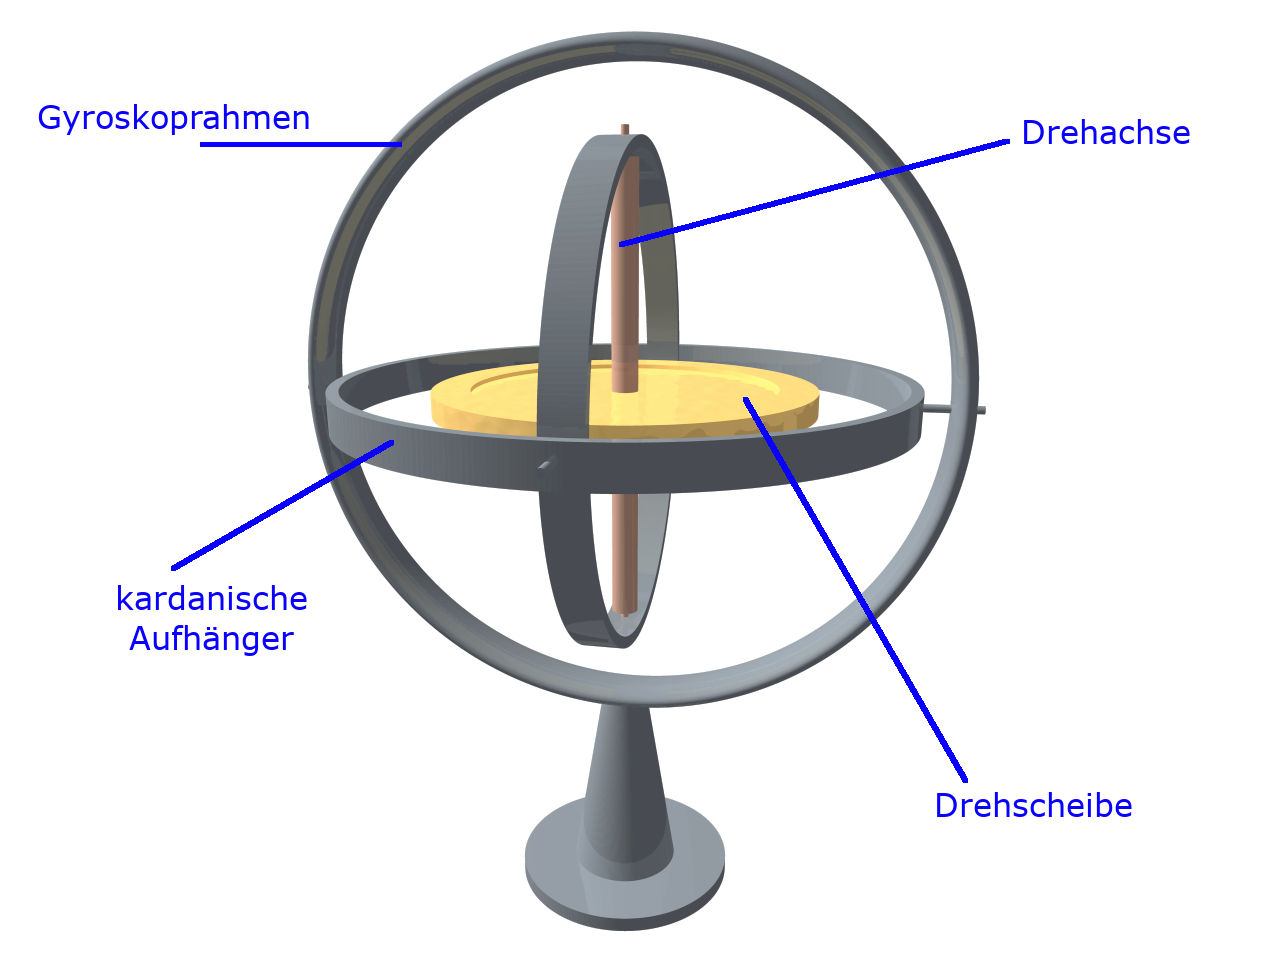
\includegraphics[width=0.5\linewidth]{Bilder/Grundlagen/3D_Gyroscope.png}
 \caption{Natürliche form von Gyroskope \cite{wikiGyroskope.2021}}
 \label{fig:gyroscope}
\end{figure}
Der Aufbau solcher Messinstrumente wird gegenwärtig als kleines Mikro Elektro Mechanisches System ausgeführt und werden MEMS-Sensoren (engl. Micro Electro Mechanical Systems) genannt. Oft werden Gyroskope zusammen mit linearen Beschleunigungssensoren als eine Komponente vermarktet. Diese Sensoren werden IMU (engl. inertial measurement unit) genannt und werden als MEMS-Sensoren entworfen. \cite[S.31f]{RobotikSichtInformatik.2012} 

% \subsection{IMU}
% Die Interne Sensoren messen physikalische Größen, die in einem Roboter zustande kommen. Dabei werden oft die Roboterorientierung und Geschwindigkeit gemessen. Die Kombination von Sensoren wie Gyroskop (siehe \autoref{subsubsec:gyroskope}) und Beschleunigungssensor (siehe \autoref{subsubsec:beschleunigungssensor}) werden zusammen als eine Einheit vermarktet diese werden als IMU bezeichnet. 
% \subsubsection{Beschleunigungssensor} \label{subsubsec:beschleunigungssensor}

\subsection{Kamera}
Die Kamera ist in seiner atomaren Struktur ein Gebilde aus Sensoren. Dabei werden Momentaufnahmen als einzelne Bilder dargestellt. So besteht ein Bild aus mehreren Rastern, die ein Abbild der einzelnen Sensoren sind. Dementsprechend werden die einzelnen Elemente des Bildes, Pixel oder Bildpunkte genannt. Im Grunde werden bei der Bildaufnahme die Sensoren mit der bestimmten Belichtungszeit bestrahlt und wandeln diese Lichtintensität in ein elektrisches Signal um. Die einzelnen Bildpunktsensoren sind letztlich Halbleitersensoren aus Silizium wie CCD-Sensor oder CMOS-Sensor. 
\begin{table}[H]
% \centering
\begin{tabular*}{\linewidth}{p{0.3\linewidth}|p{0.3\linewidth}|p{0.3\linewidth}}
\hline
\textbf{Prinzip}          & \textbf{CCD}         & \textbf{CMOS}        \\ \hline\hline
Pixelsignal      & Ladungen     & Spannungen   \\ \hline
Arbeitsweise     & Integrierend & Proportional \\ \hline
Rauschpegel      & Gering       & Mittel       \\ \hline
Gleichförmigkeit & Hoch         & Gering       \\ \hline
Geschwindigkeit  & Mittel       & Hoch         \\ \hline
Kosten           & Mittel       & Gering       \\ \hline
\end{tabular*}
\caption{Gegenüberstellung der CCD- und CMOS-Sensoren \cite[S.371]{SensorenAutomation.2014}}
\label{tab:vergleichCCD_CMOS}
\end{table}
Die CCD-Sensoren arbeiten anders als CMOS-Sensoren (siehe \autoref{tab:vergleichCCD_CMOS}), die einzelnen Ladungen der Sensoren werden in kleinen Zeitabständen ausgelesen, indem die Ladungen durch ein Schieber Register verschoben werden. Diese Methode ist auch der Namensgeber für CCD-Sensoren (engl. Charged Coupled Devices). Bei der Ladungsübertragung gibt es zwei Typen Frame-Transfer-Typen, die über Zwischenspeicher das gesamte Bild in einem Takt übertragen, und Interline-Transfer-Typen, die zeilenweise zum Ausgangsregister ausgelesen werden. Gegenübergestellt werden bei CMOS-Sensoren die Ladungen direkt am Bildpunkt abgeholt und in eine analoge Spannung gewandelt. So besteht beim CMOS-Sensor jeder einzelne Sensor aus Signalverstärkern aus mehreren Transistoren. Die in dieser Arbeit verwendete Kamera ist eine Raspberry Pi Kamera, die mit CMOS-Sensoren arbeitet. 

\section{Navigation}\label{subsec:Navigation}
Eine entscheidende Aufgabe eines mobilen Roboters ist die Navigation. Dazu muss ein mobiler Roboter sich frei und kollisionsfrei in der Umgebung bewegen. Die Navigation beinhaltet Zusammensetzungen aus Selbstlokalisierung, Kartenerstellung und Pfadplanung. Die Selbstlokalisierung und Kartenerstellung ist in der Literatur mit dem Erkenntnis SLAM abgefasst. Dieses Verfahren ist nicht Teil dieser Arbeit und wird nicht näher erläutert. In den folgenden Kapiteln wird auf die relative Navigation und den Pledge-Algorithmus eingegangen.\autocites[S.261ff]{RobotikSichtInformatik.2012}[S.97f]{MobileRobotikEinfuehrung.2002}
\subsection{Relative Navigation}
Als relative Navigation wird verstanden, dass sich das Vehikel im Hinblick zu seinem Umfeld fortbewegt. Die einfachste Form ist, dass der mobile Roboter sich dort hinbewegt, wo keine Hindernisse zu erkennen sind. In der Literatur wird diese Art der Navigation auch Freiraumnavigation genannt. Die Idee dieser Navigation ist es, dass sich das Vehikel im freien Raum bewegt und die Richtung stabil hält, wobei Hindernissen ausgewichen wird, ohne in Schwingung zu kommen. Solche Oszillationen kommen zustande, wenn die Programmierung direkt auf die Sensoren reagiert als Reflex, ohne eine Regelung.
Dabei kann eine Fuzzy Regelung herangezogen werden wie die in der \autoref{lst:fuzzy}, sie gibt an, in welche Richtung der Roboter fahren soll mit i-ten Abstandswert vom Laserscanner. 
\lstset{
    basicstyle=\ttfamily,
    showstringspaces=false,
    commentstyle=\color{olive},
    keywordstyle=\color{blue},
    breaklines=true,
    literate={ß}{{\ss}}1
}
 \begin{lstlisting}[caption={Fuzzy Regelung \cite{RobotikSichtInformatik.2012, S.266}}, label={lst:fuzzy},captionpos=b,xleftmargin=.3\linewidth]
 WENN(Winkel_i ist in Fahrtrichtung) UND
    (Entfernung_i ist groß) 
 DANN fahre in diese Richtung
 \end{lstlisting}

Eine beispielhafte Relative Navigation kann wie folgendermaßen beschrieben werden. Der Roboter fährt so lange geradeaus, bis er auf ein Hindernis trifft. Dabei kann die Vorwärts Geschwindigkeit sofort auf 0 gesetzt werden, wenn die Distanz einen Schwellwert unterschreitet und zugleich wird eine Drehung mit konstanter Geschwindigkeit gestartet, bis die Sicht frei wird. Das Tempo vom Roboter kann durch eine einfache Formel skaliert werden (siehe \autoref{regelungGeschwindigkeit}), wenn die Distanz zum Objekt kleiner ist als die maximale Distanz, dann wird das Tempo verhältnismäßig geregelt, doch falls alles frei ist, wird mit dem größten Tempo gefahren. 

\begin{align}\label{regelungGeschwindigkeit}
\centering
\begin{split}
v_{current} &= (d_{current}/d_{max}) \cdot v_{max}
\end{split}
\end{align}

Die Idee hinter der Freiraumnavigation ist das Spurfahren im Straßenverkehr. Die Geschwindigkeit soll nicht beeinflusst werden, solange die Spur des Fahrzeuges frei ist. \cite[S.266 ff]{RobotikSichtInformatik.2012}

% \lstset{
%     language=python,
%     basicstyle=\ttfamily,
%     showstringspaces=false,
%     commentstyle=\color{olive},
%     keywordstyle=\color{blue},
%     breaklines=true,
% }
%  \begin{lstlisting}[caption={ein paar Zeilen code}\label{lst:test123},captionpos=b] 
%  def moveRobotRelative():
%     maxSpeed = 1.0 # 1 m/s
%     maxDistance = 1.2 #1m
%     minDistance = 0.60 #60cm
%     currentForwardSpeed = 0
%     distanceForward = lidarDistance[160:200] #lidar werte von der Roboterfrontseite mit +20 und -20 Grad 
    
%     if(np.median(distanceForward) < minDistance):
%         currentForwardSpeed = 0
%         robot.setSpeed(currentForwardSpeed)
%         robot.rotateUntilFrontFree()
%     else:
%         if(np.median(distanceForward) < maxDistance):
%             currentForwardSpeed = (np.median(distanceForward)/maxDistance) * maxSpeed
%         else:
%             currentForwardSpeed = maxSpeed
        
%         if(np.median(distanceForward) < minDistance):
%             currentForwardSpeed = 0
%     robot.setSpeed(currentForwardSpeed)
        
%  \end{lstlisting}

\subsection{Pledge-Algorithmus} \label{Pledge_Algo}
Es gibt verschiedene Methoden, um aus einem Labyrinth zu entkommen wie zum Beispiel die Tiefensuche, Linke- bzw. Rechte-Hand-Regel oder Pledge Algorithmus, der hier näher dargelegt wird. Der Algorithmus wurde nach dem Erfinder John Pledge einem zwölfjährigen Jungen benannt. Pledge Algorithmus funktioniert in jedem Labyrinth das rechtwinklige Ecken hat und erweitert die Linke- bzw. Rechte-Hand-Regel. 

\begin{figure}[h]
  \centering
  \subfloat[][]{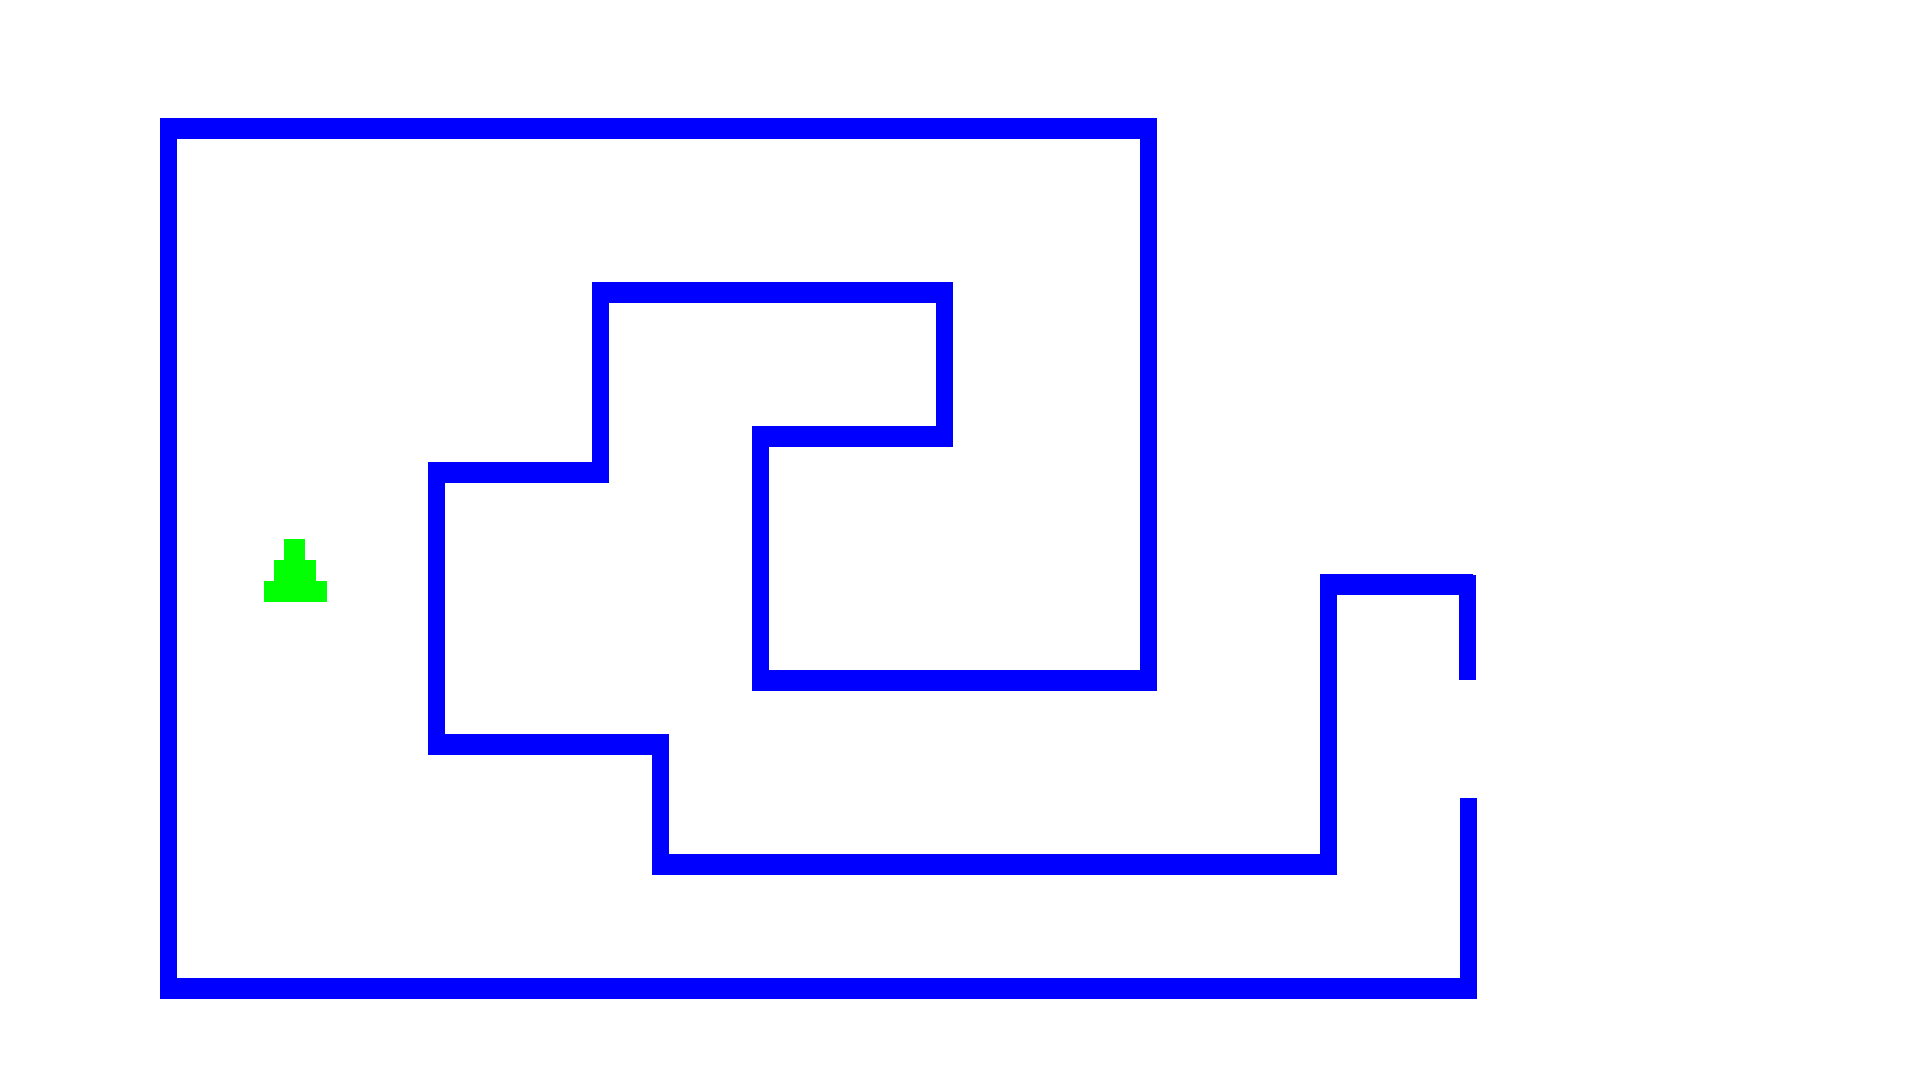
\includegraphics[width=0.4\linewidth]{Bilder/Grundlagen/Pledge/L1.png}}%
  \qquad
  \subfloat[][]{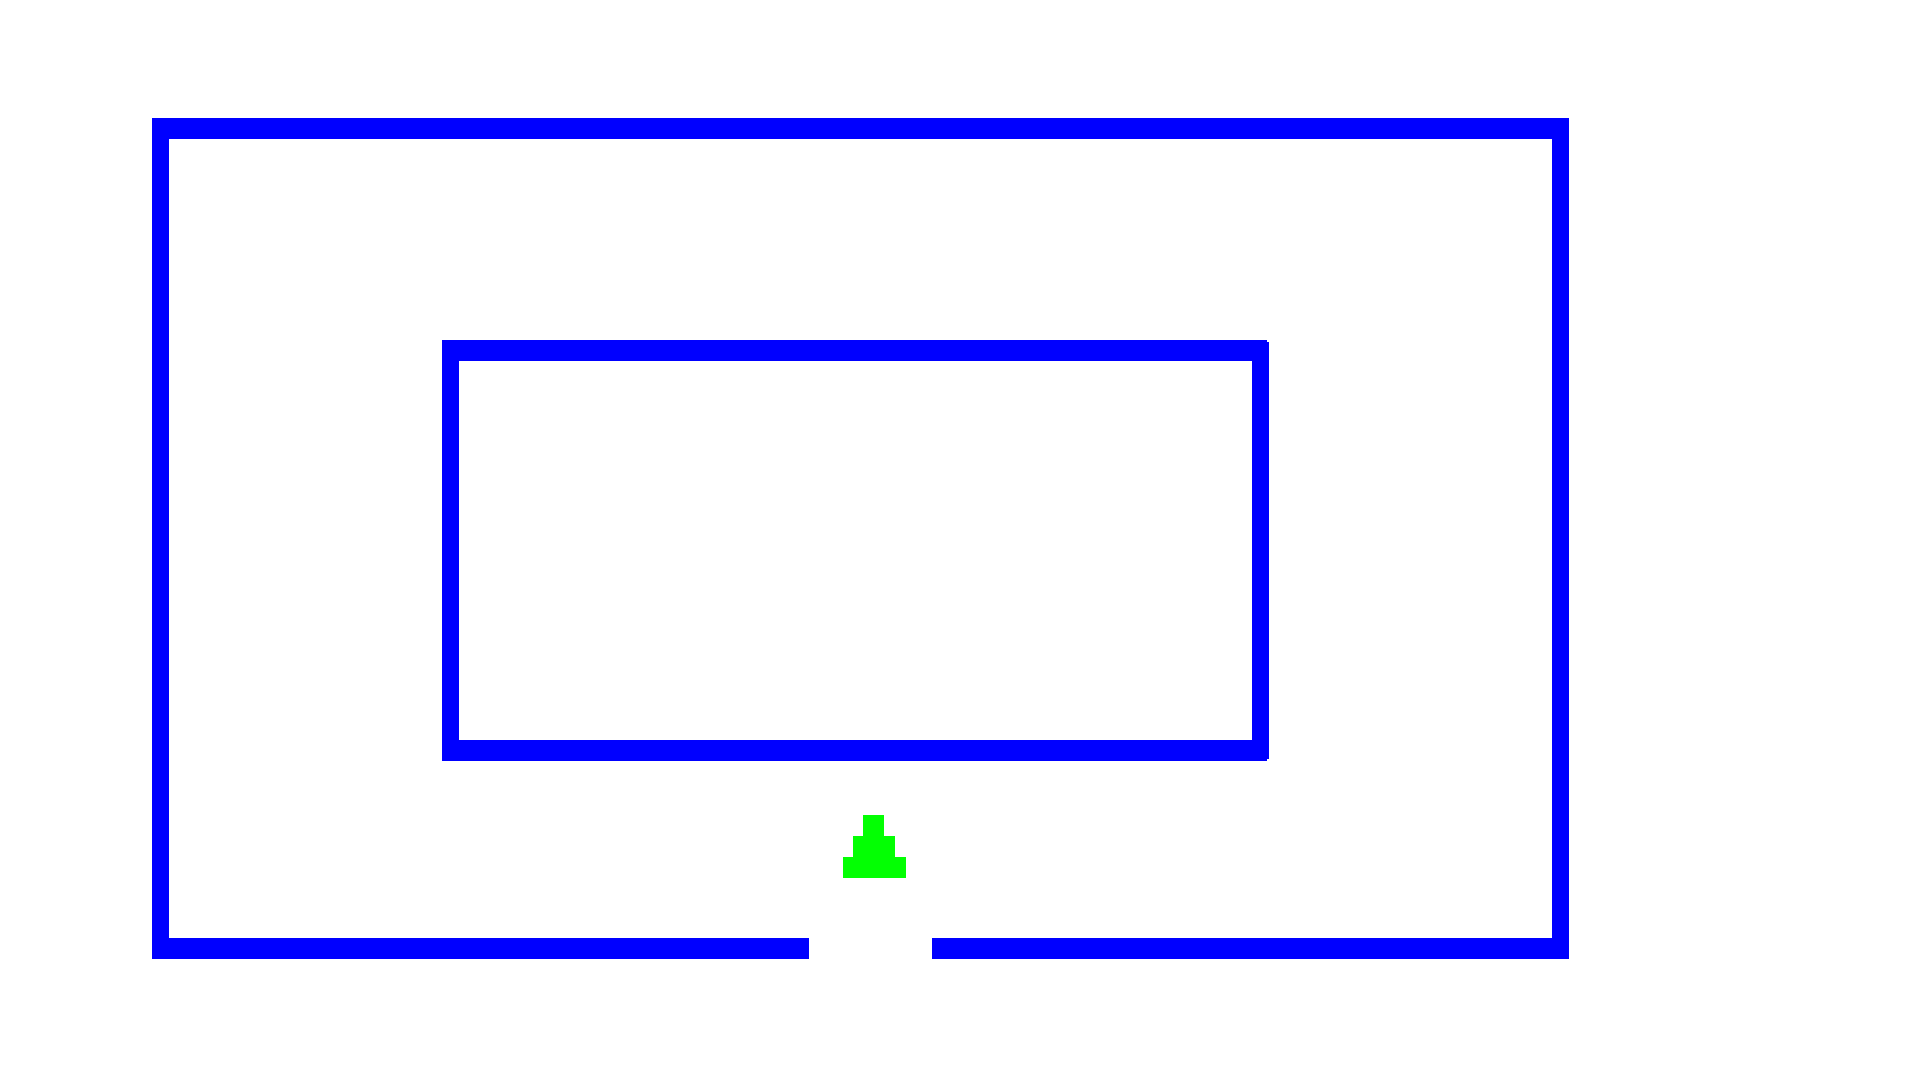
\includegraphics[width=0.4\linewidth]{Bilder/Grundlagen/Pledge/L2.png}}%
  \caption{Labyrinth}
  \label{fig:Labyrinth}
\end{figure}

Die Grundidee ist bei der Hand-Regel, die Wand mit der Hand so lange zu verfolgen, bis ein Ausweg gefunden wird (siehe \autoref{fig:LinkeRechteHandRegel}[a]). Diese Idee funktioniert nicht, wenn es auf eine Säule trifft, denn dann dreht sich der Durchläufer im Kreis (siehe \autoref{fig:LinkeRechteHandRegel}[b]).
\begin{figure}[H]
  \centering
  \subfloat[][]{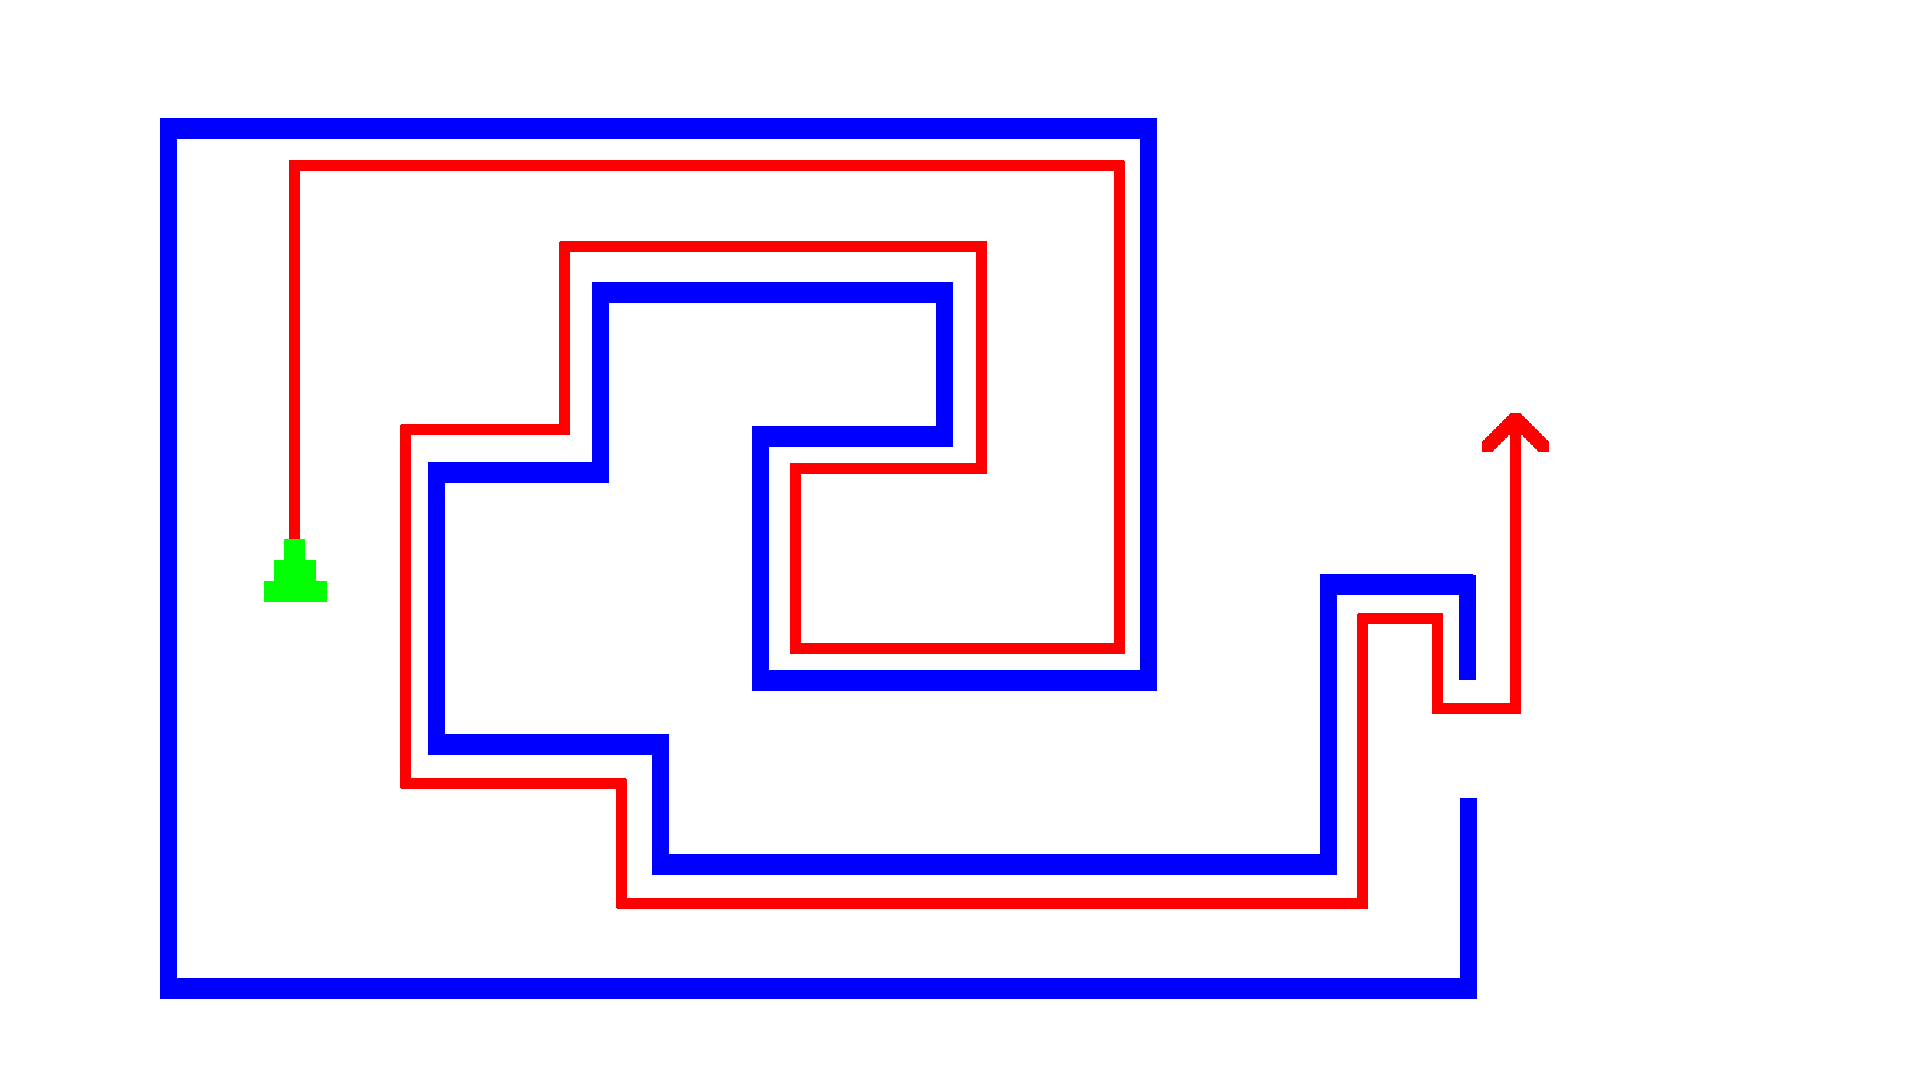
\includegraphics[width=0.4\linewidth]{Bilder/Grundlagen/Pledge/L1_O_P_Linkehand.png}}%
  \qquad
  \subfloat[][]{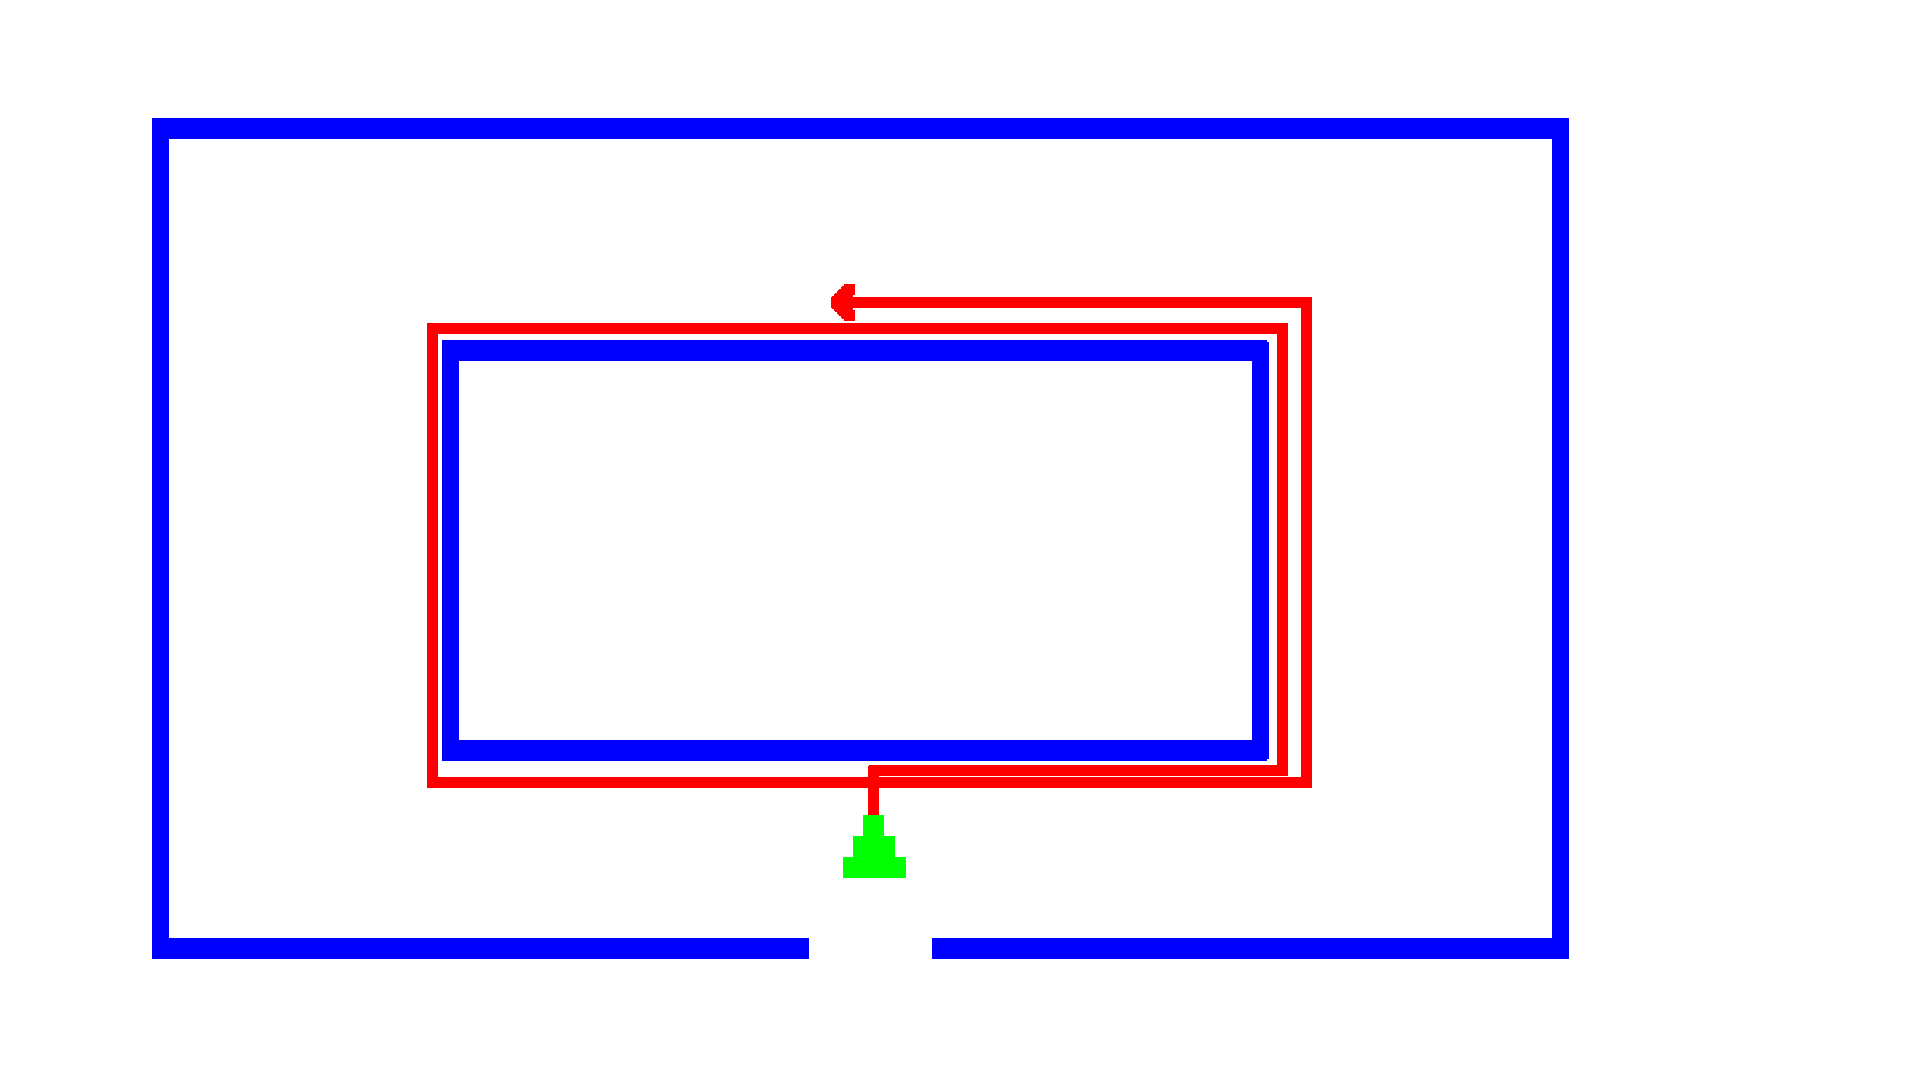
\includegraphics[width=0.4\linewidth]{Bilder/Grundlagen/Pledge/L2_O_P.png}}%
  \caption{Grundidee Linke- bzw. Rechte-Hand-Regel}
  \label{fig:LinkeRechteHandRegel}
\end{figure}

Eine weitere Funktionalität, die diesen Algorithmus erweitern kann, ist die, dass der Durchläufer seine Start Orientierung speichert und beim Laufen im Kreis die Wand verlässt, wenn die aktuelle Orientierung der Start Orientierung entspricht. Diese Funktion hilft beim Laufen im Kreis bei Säulen aber nicht immer bei allen Labyrinthen und führt zu Fehlfunktionalität.
\begin{figure}[H]
  \centering
  \subfloat[][]{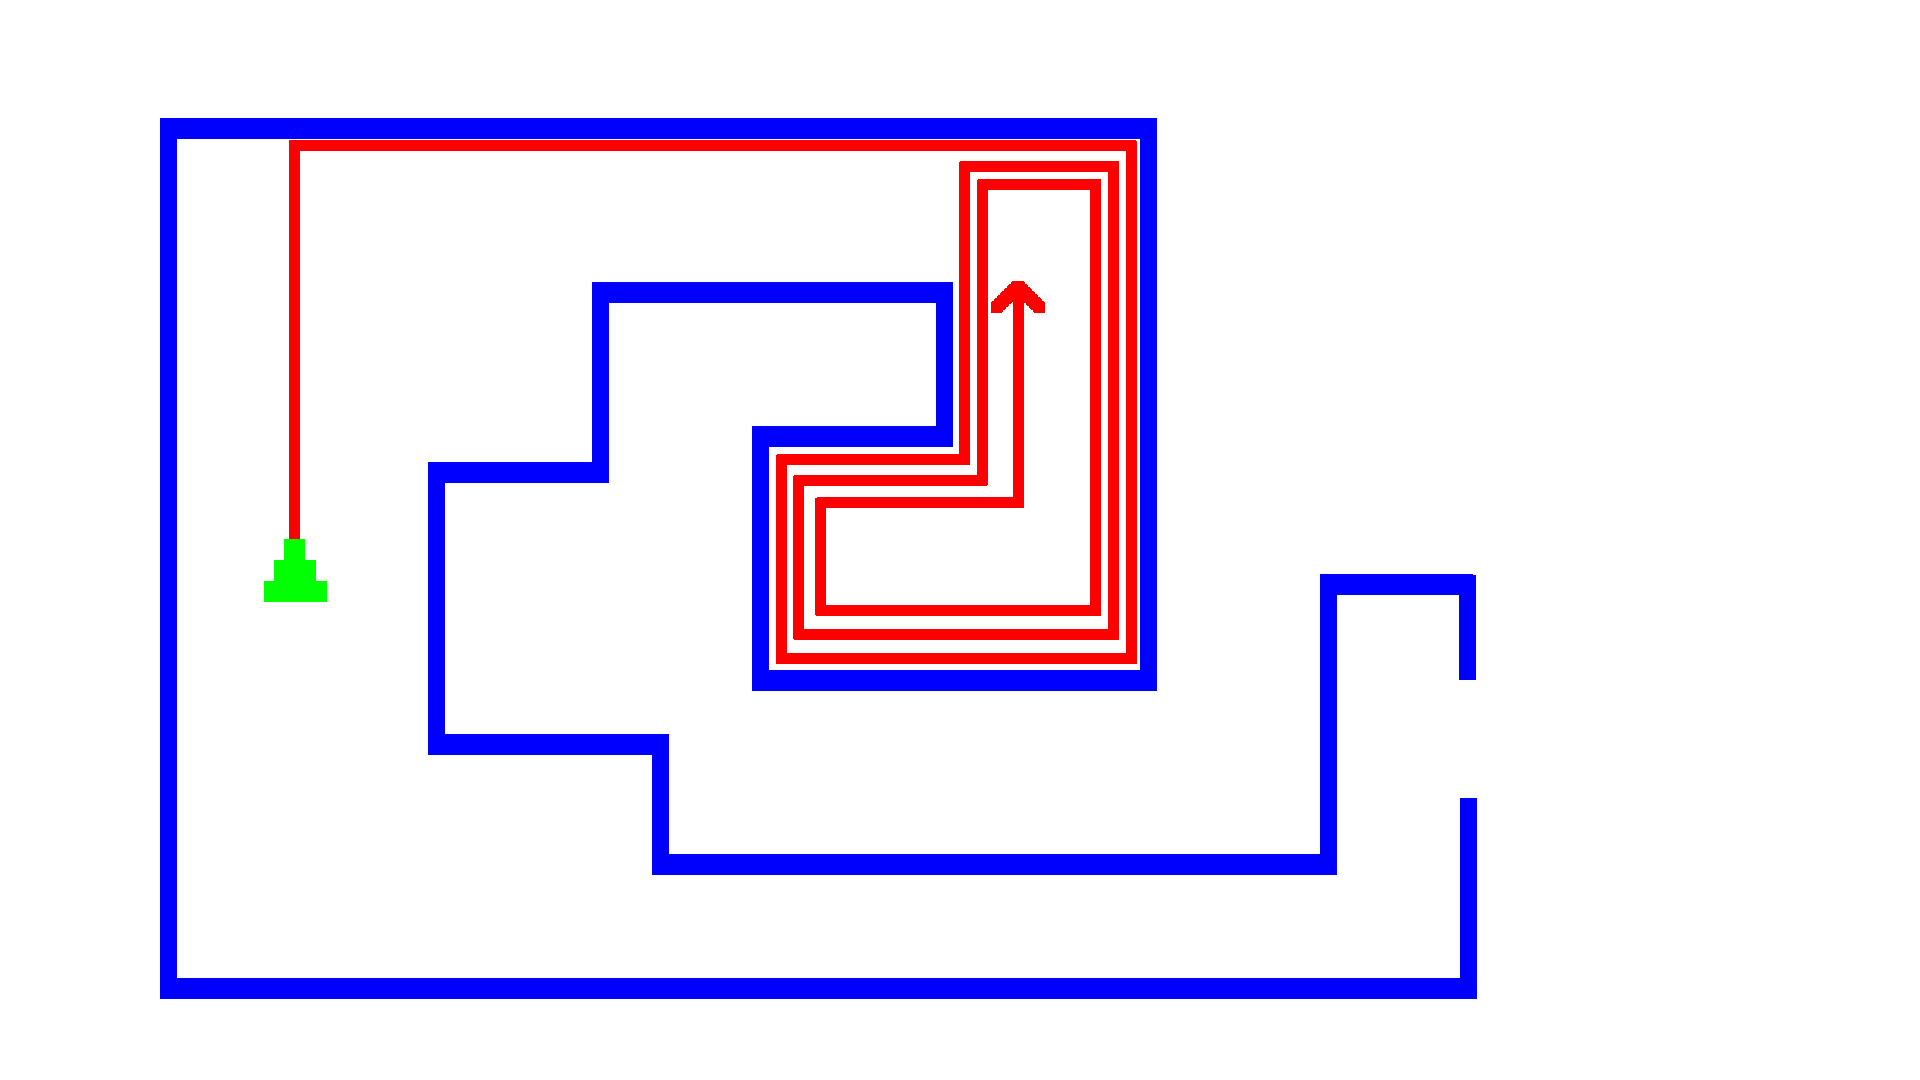
\includegraphics[width=0.4\linewidth]{Bilder/Grundlagen/Pledge/L1_O_P.png}}%
  \qquad
  \subfloat[][]{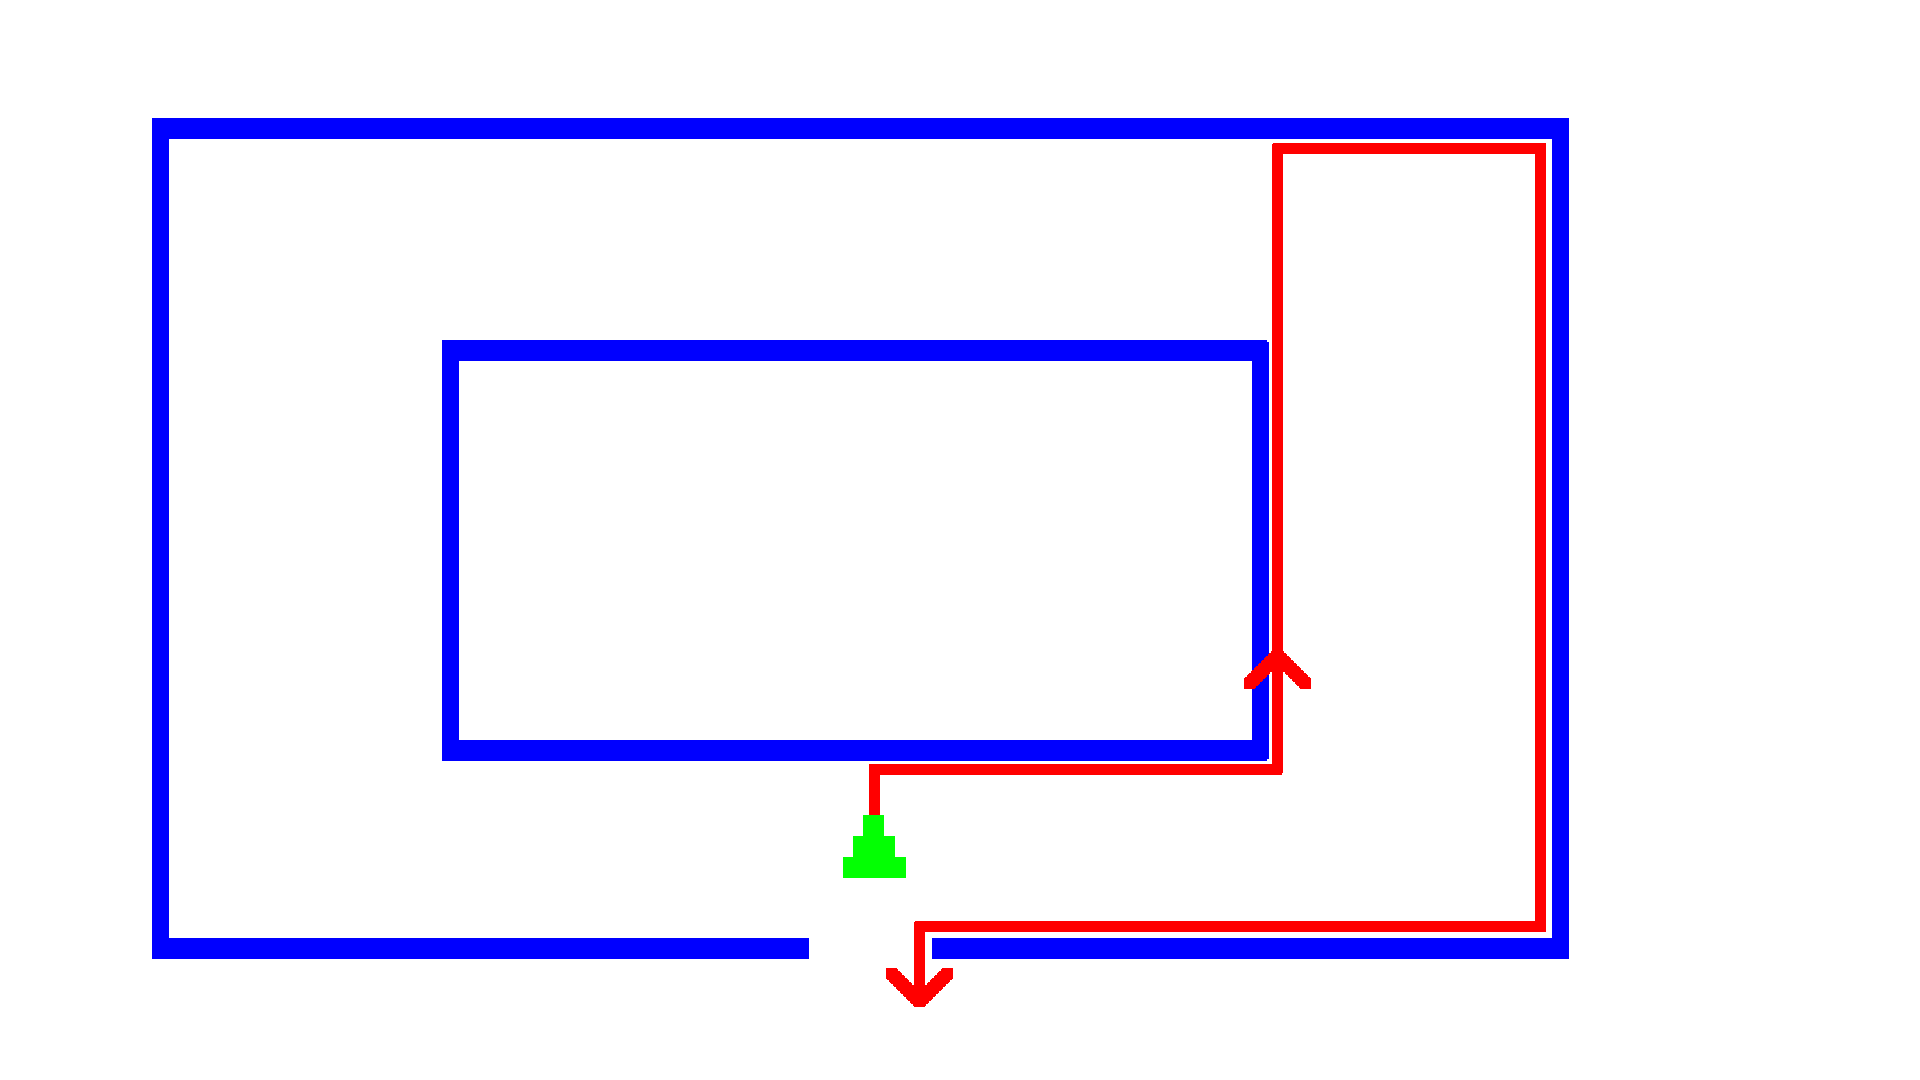
\includegraphics[width=0.4\linewidth]{Bilder/Grundlagen/Pledge/L2_O_P_Linkehand.png}}%
  \caption{Linke- bzw. Rechte-Hand-Regel mit Erweiterung Start Orientierung Speicherung}
  \label{fig:StartorientierungSpeicherung}
\end{figure}
Diese ganzen Funktionalitäten werden beim Pledge-Algorithmus verbessert und so durch alle Irrgärten, die einen Ausgang besitzen, herausfinden. Beim Pledge Verfahren gibt es zwei entscheidende Regeln.
\begin{enumerate}
    \item Geradeaus fahren oder Laufen bis eine Wand erreicht wird.
    \item Die Wand verfolgen, bis der Umdrehungszähler gleich null wird. 
\end{enumerate}

\begin{figure}[H]
  \centering
  \subfloat[][]{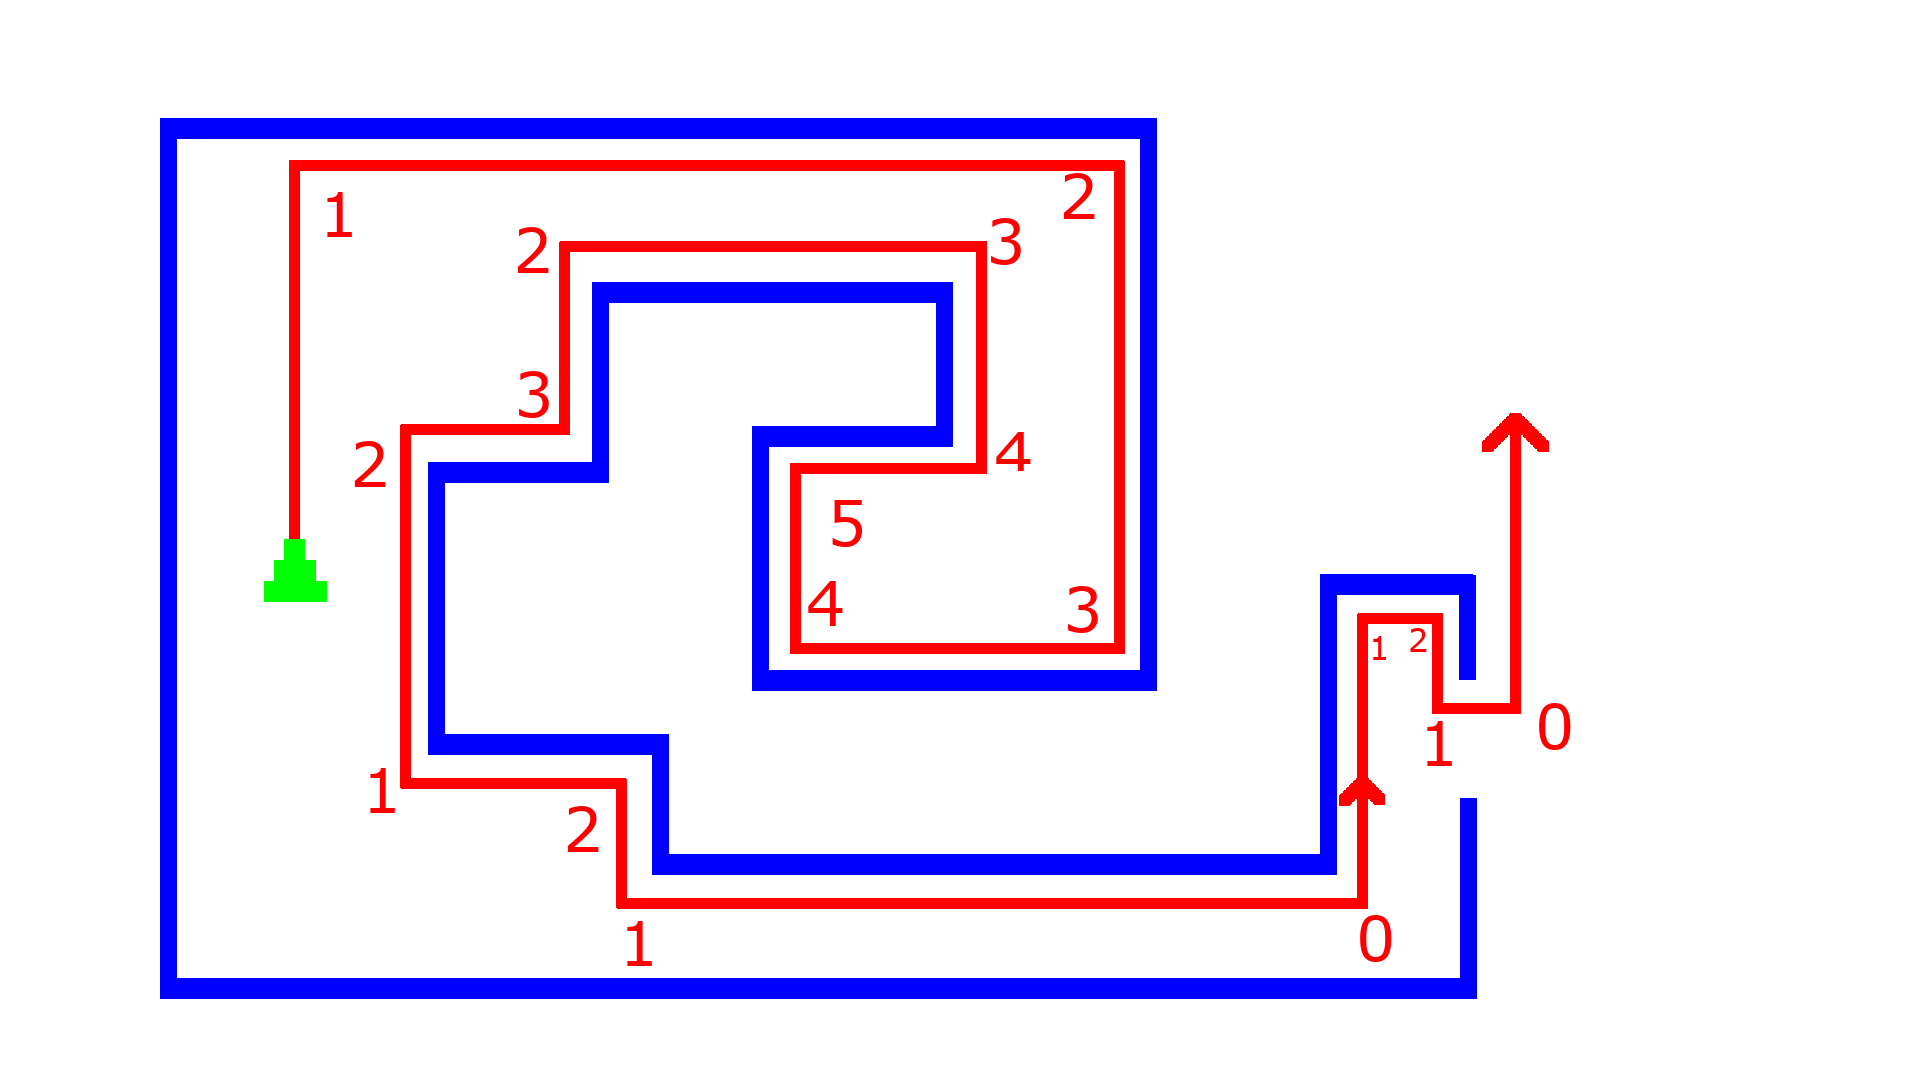
\includegraphics[width=0.4\linewidth]{Bilder/Grundlagen/Pledge/L1_M_P.png}}%
  \qquad
  \subfloat[][]{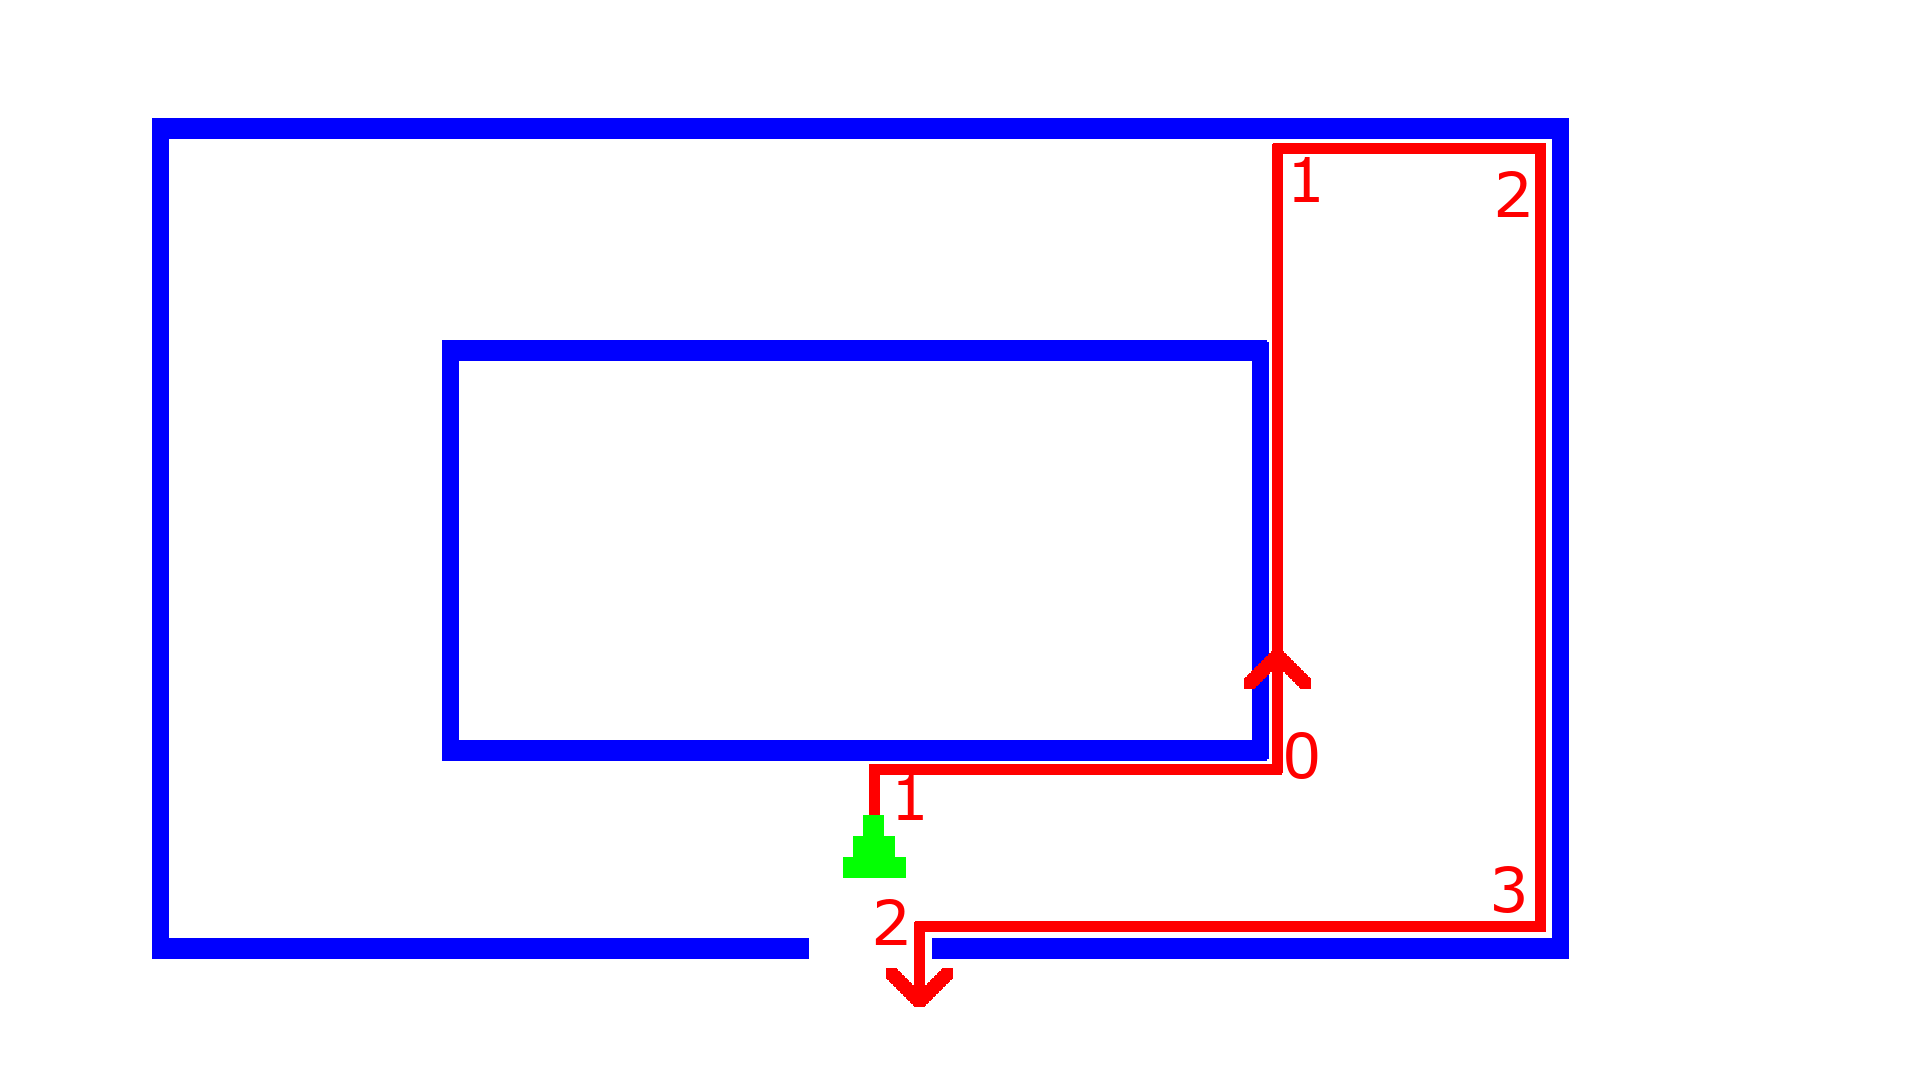
\includegraphics[width=0.4\linewidth]{Bilder/Grundlagen/Pledge/L2_M_P.png}}%
  \caption{Ablauf Pledge-Algorithmus an zwei Labyrinth Typen}
  \label{fig:PledgeAlgo}
\end{figure}

Diese Regeln werden beim Plege-Algorithmus iteriert, bis ein Ausweg gefunden wird (siehe \autoref{fig:PledgeAlgo}). Falls es keinen Ausweg gibt, wird je nach Definition im Uhrzeigersinn oder gegen den Uhrzeigersinn gedreht und der Winkelzähler immer weiter erhöht bzw. verringert. \cite[S.75 ff]{HandbuchAlgorithmen.2008}\cite[S.250 ff]{AlgoIng.2018}\cite[S.318 ff]{AlgoGeo.2005}

\input{Abschnitte/Projektdurchführung}
\chapter{Ergebnisse und Diskussion}

Im folgenden Kapitel werden die Ergebnisse aus der Entwicklung zusammengefasst, im Gesamtzusammenhang dieser Arbeit interpretiert und mögliche Ansätze für weitere Forschung aufgezeigt. \\

 Wie in der Zielsetzung \autoref{sect:Zielsetzung} beschrieben wurde ging es in dieser Arbeit um eine Analyse und eine prototypische Entwicklung eines Systems das dazu dienen soll, eine Schnittstelle zu schaffen, die genutzt werden kann um mobile Roboter einfacher zu steuern ohne Kenntnisse mit Roboterkontrollarchitekturen. Es können verschiedene Szenarien als Benutzeroberflächen genutzt werden mit ein und derselben Anwendungsschnittstelle, so kann spielerisch die Funktionalität von Robotern näher gebracht werden. Die Intelligenz von mobilen Robotern kann je nach Anwendung so übermittelt werden. Dabei ergibt sich die Frage, warum wurde solch eine Arbeit durchgeführt da es schon Roboter Systeme gibt wie zum Beispiel von LEGO die genau dieses Vorhaben ermöglichen. Die Antwort dazu ist einfach, es gibt verschiedene Systeme die genau das Thema dieser Arbeit decken aber leider sind solche Systeme gebunden an Hersteller und es gibt nicht viel Spielraum für Erweiterung und Anwendungsgebiete. So ist es bei LEGO notwendig die eigenen Produkte zu verwenden sowohl Hardware oder Software. In erster Linie soll es als Exponat für die Firma Kurt Hüttinger GmbH dienen und Kindern aber auch erwachsenen Personen die heutzutage mögliche Intelligenz von mobilen Robotern vermitteln. Das API das hier entwickelt wurde kann durch die offene Gestaltung und durch die Standard Netzwerkprotokolle wie TCP und UDP eine beliebige Benutzeroberfläche nutzen (siehe \autoref{fig:gui_api_robot}). 
 
 \begin{figure}[H]
 \centering
 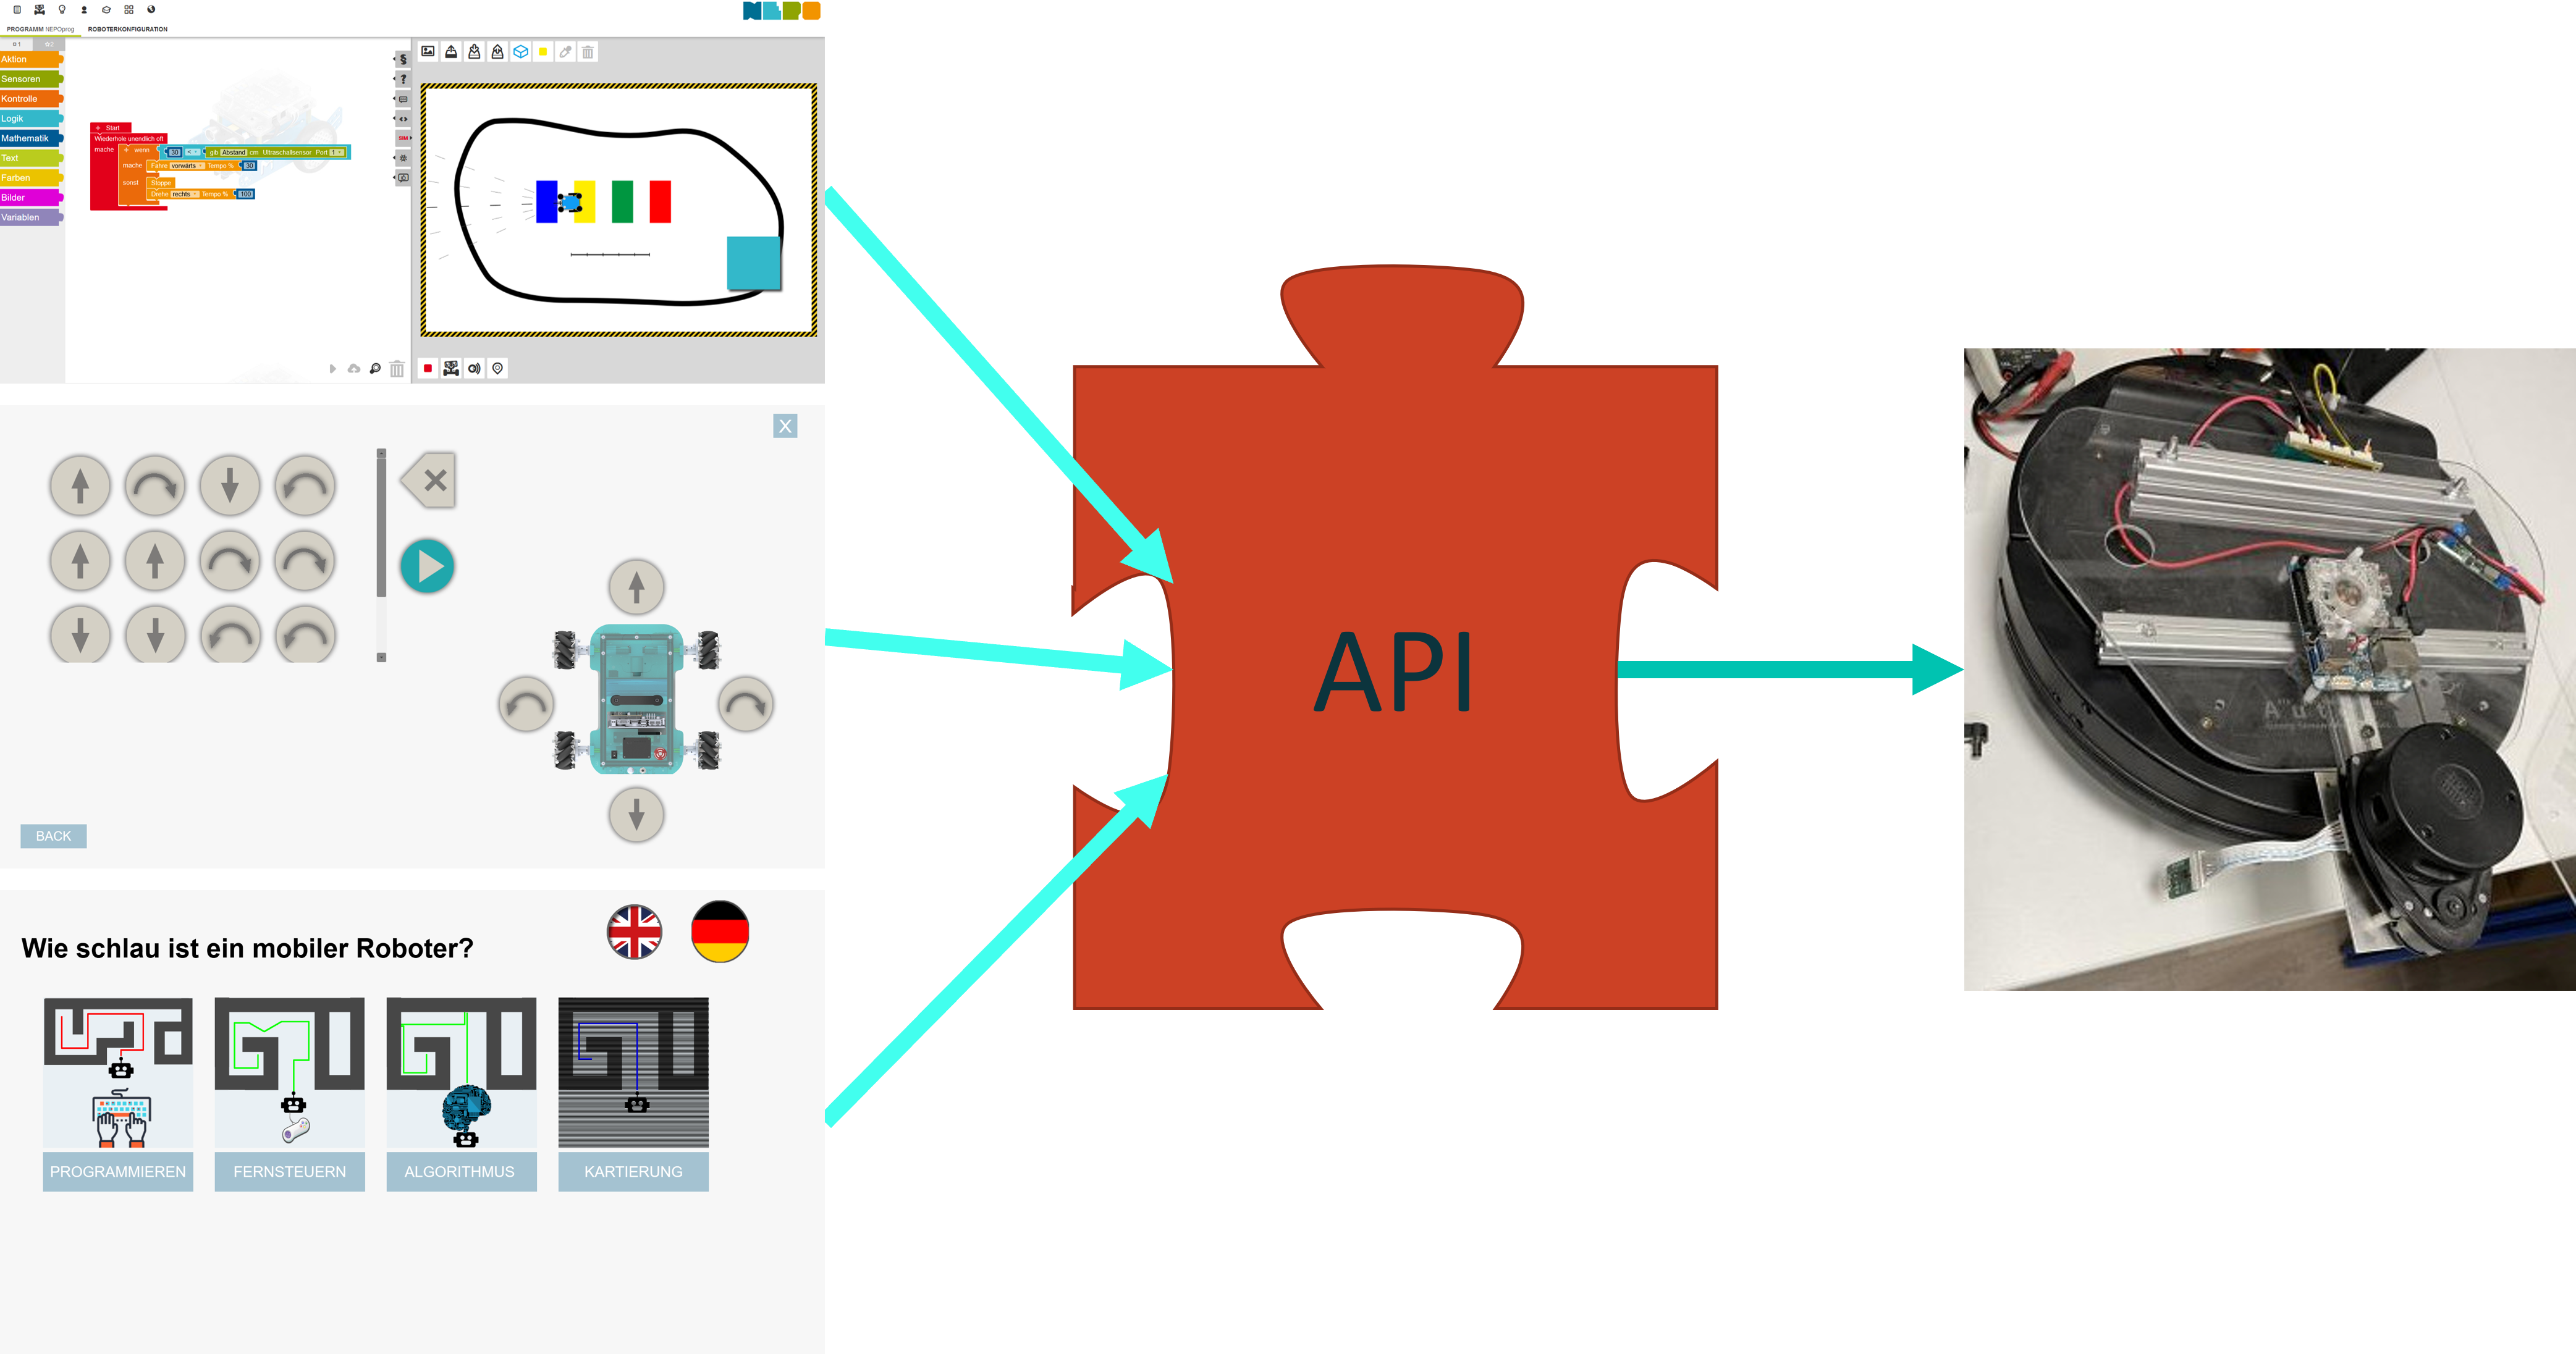
\includegraphics[width=\linewidth]{Bilder/Ergebnisse/gui_api_robot.png}
 \caption{Vereinfachte Darstellung der Kommunikation mit der API}
 \label{fig:gui_api_robot}
\end{figure}
 
Des weiteren konnte ein Ansatz für einen Algorithmus entwickelt werden der dazu dient den mobilen Roboter aus einem benutzerdefinierten Hindernisparcours zu befreien. Durch solche intelligenten Funktionalitäten können die Möglichkeiten des Machbaren an die anwendenden Personen transportiert werden. Dabei schafft diese Arbeit eine Basis und einen Grund-Wissenslevel der für weitere Funktionalitäten genutzt werden kann.
 
Die Arbeit behandelte viele kleine Punkte, die zu diesem Ergebnis führten. So konnte eine Basis geschaffen werden, die zur Weiterentwicklung herangezogen werden kann. Es können weitere Intelligenzen des mobilen Roboters implementiert werden und so spielerisch der Wissensstand der Forschung auf dem Gebiet der mobilen Roboter übermittelt werden. Die weiteren Anknüpfungspunkte dieser Arbeit könnten Kartierung mithilfe von SLAM sein. So kann durch Kartenbildung eine schnellere Navigation zur Ladestation erfolgen. Die Kartenbildung könnte sich beim Plegde-Algorithmus im Hintergrund aufbauen und im Anschluss könnte durch einen anderen Algorithmus wie \textit{A-Star} oder \textit{Dijkstra} der Pfad zurück zum Start gefunden werden.  
\chapter{Tests}
In diesem Kapitel werden die Tests näher erläutert, die während der Implementierung des Systems durchgeführt wurden.

\section{Test mit der ROS Umgebung}

Die Roboterkontrollarchitektur ROS hat für die Entwicklung verschiedene Tools zur Verfügung. Dazu können grafische und auch Befehlszeile Programme verwendet werden, um das laufende System zu Debuggen.\\
Ein grafisches Programm ist \textit{RVIZ}, das 3-D-Visualisierung von Sensordaten, Robotermodellen und anderen 3-D-Daten ermöglicht. Durch diese Software konnten Sensordaten visualisiert und somit geholfen werden, die Implementierung greifbarer zu machen. So konnte schnell entdeckt werden, dass der LiDAR Scanner bei Messungen seitlich des Roboters Probleme aufzeigt.\\
Die \textit{rqt\_graph} ist ein Tool, um die aktiven Knoten, Topics und deren Verbindung grafisch als Diagramm darzustellen. Damit konnte in der Entwicklung zur Laufzeit aufgezeigt werden, wie die einzelnen Topics miteinander kommunizieren. Bei falscher Schreibweise der Topics führt es nicht in erster Linie zum Fehler, sondern zu neuen Topics die nicht existieren. Um solche Inkorrektheit zu sehen, kann diese Software verwendet werden. So kann durch die Darstellung der Verbindungen auch auf den ersten Blick gesehen werden, welche Verbindungen nicht stimmen. \\
Weitere Werkzeuge sind die Befehlszeilen-Tools. Sie ermöglichen zur Laufzeit Informationen zu den einzelnen Knoten, Topics oder Nachrichten auszugeben. Es können Sensor-Topics ausgeben werden, die während der Laufzeit überwacht werden können. Sie bieten aber auch die Möglichkeit, Verbindungen oder die Anzahl davon abzudrucken und somit eine nicht grafische Art von \textit{rqt\_graph} darstellt. Diese Kommandozeilen Werkzeuge werden häufig verwendet, da sie eine schnelle und unkomplizierte Lösung sind.

\section{API Test mit einer grafischen Oberfläche}
Um die Schnittstelle zu testen, wurde mithilfe der firmeninternen Software eine grafische Oberfläche entwickelt. Die firmeninterne Software basiert auf \textit{Windows Presentation Foundation}, kurz \textit{WPF} Anwendung und heißt \textit{Interactive Graphic Panel}, kurz genannt \textit{IGP}. Die Software ist so aufgebaut, dass im Hintergrund eine \textit{WPF} Anwendung läuft mit vielen \textit{C\#} Funktionalitäten wie TCP oder UDP Sockets, aber die grafische Benutzeroberfläche und die Interaktivität wird mit Javascript programmiert und mithilfe von \textit{XML} werden die Layouts der einzelnen Seiten erstellt. So konnte schnell eine Mensch-Maschinen-Interaktion erstellt werden, die zu Testzwecken verwendet werden konnte (siehe \autoref{fig:GUI}). \\ 

\begin{figure}[H]
\captionsetup[subfloat]{labelformat=empty}
  \centering
  \subfloat[][]{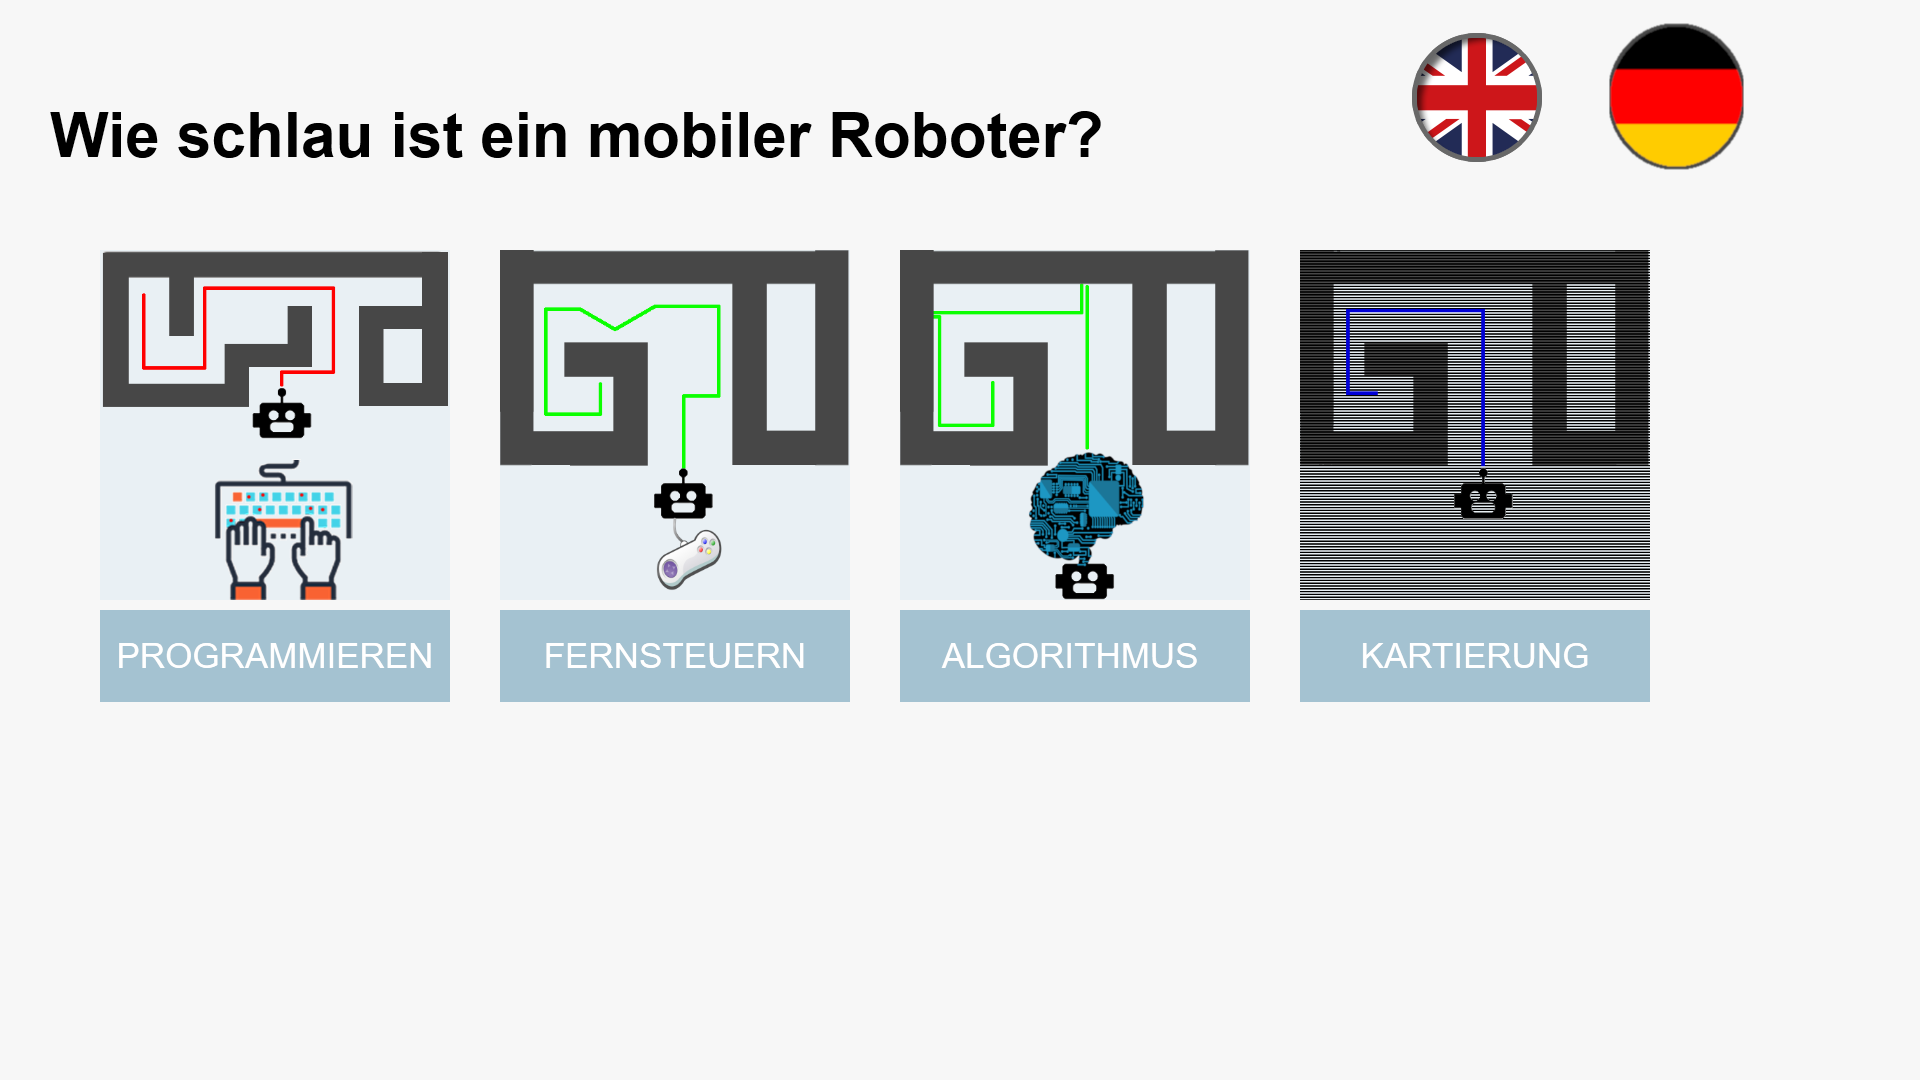
\includegraphics[width=0.5\linewidth]{Bilder/Tests/home_de.PNG}}%
  \subfloat[][]{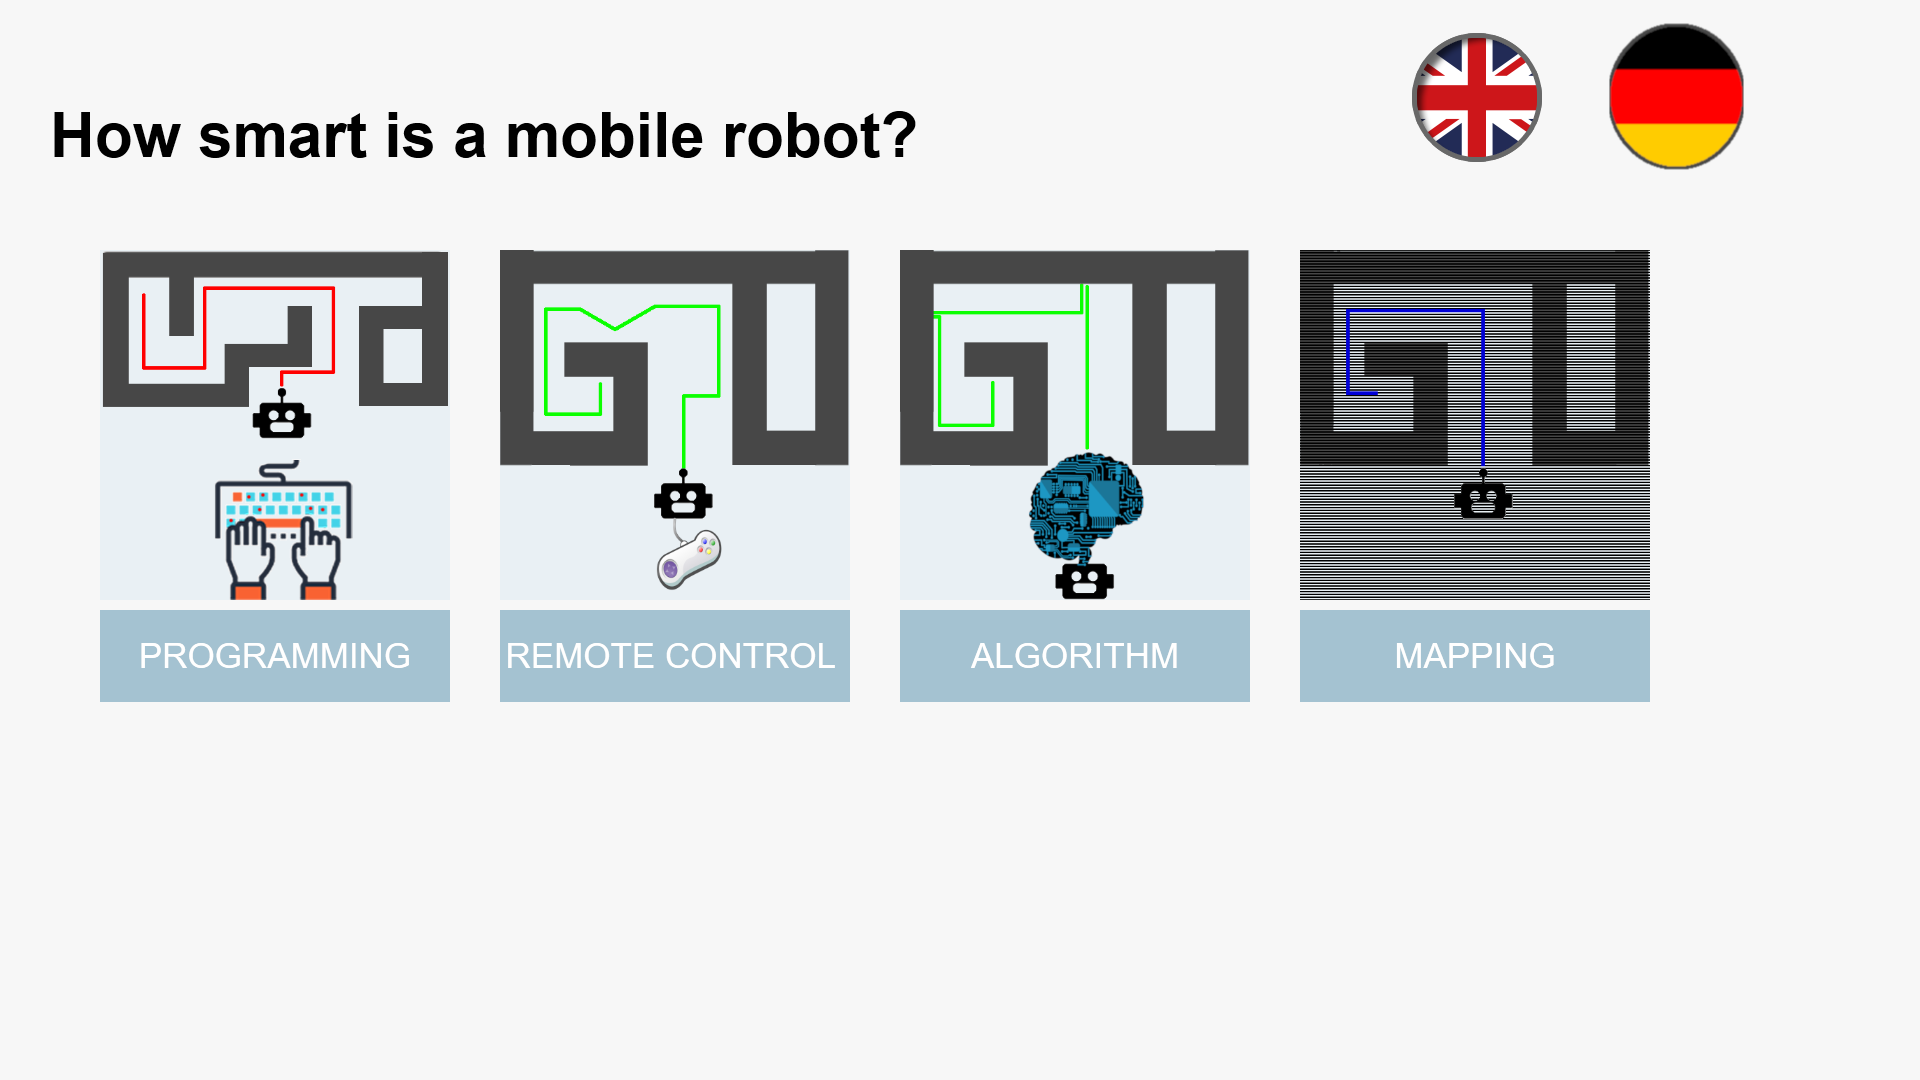
\includegraphics[width=0.5\linewidth]{Bilder/Tests/home_en.PNG}}%
  \qquad
  \subfloat[][]{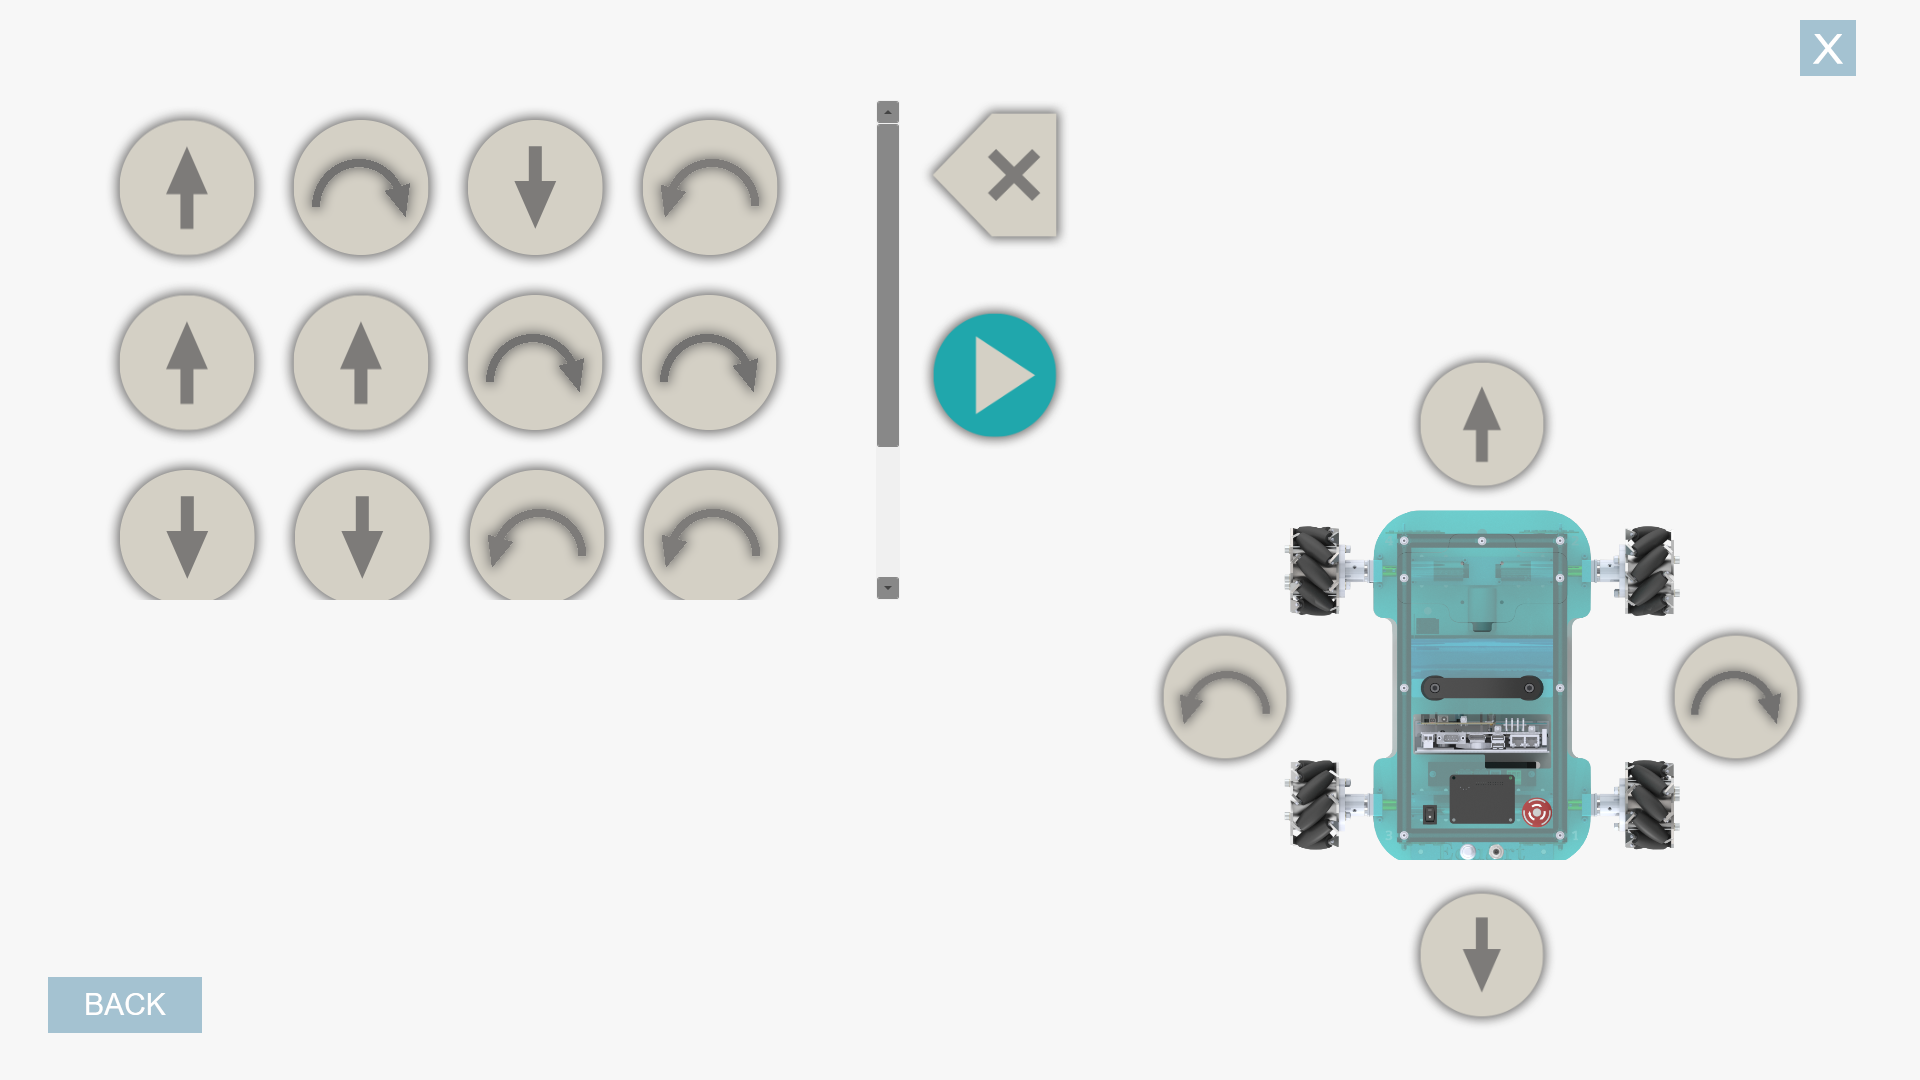
\includegraphics[width=0.5\linewidth]{Bilder/Tests/programming_scroll_scroll.PNG}}%
  \subfloat[][]{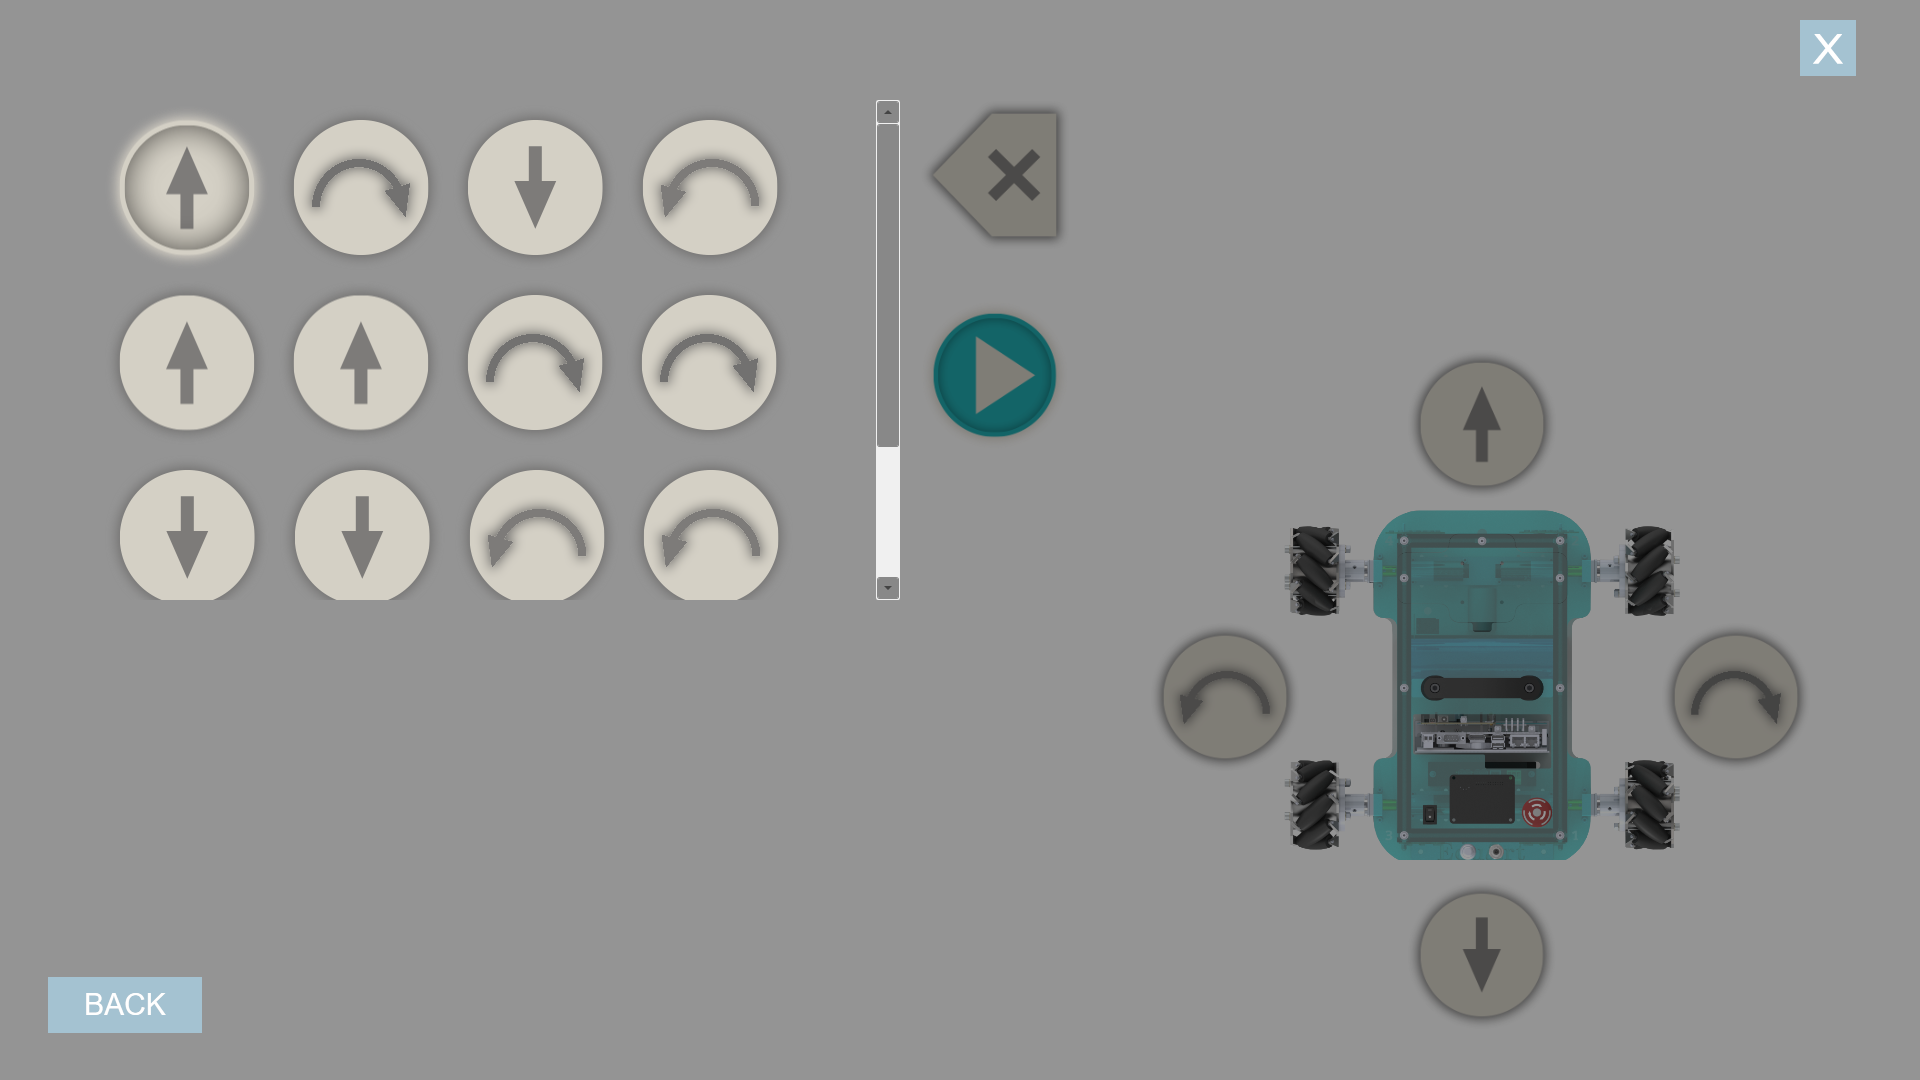
\includegraphics[width=0.5\linewidth]{Bilder/Tests/programming_aktive_scroll.PNG}}%
  \qquad
  \label{fig:GUI1}
\end{figure}

\begin{figure}[H]
\captionsetup[subfloat]{labelformat=empty}
  \centering
%   \subfloat[][]{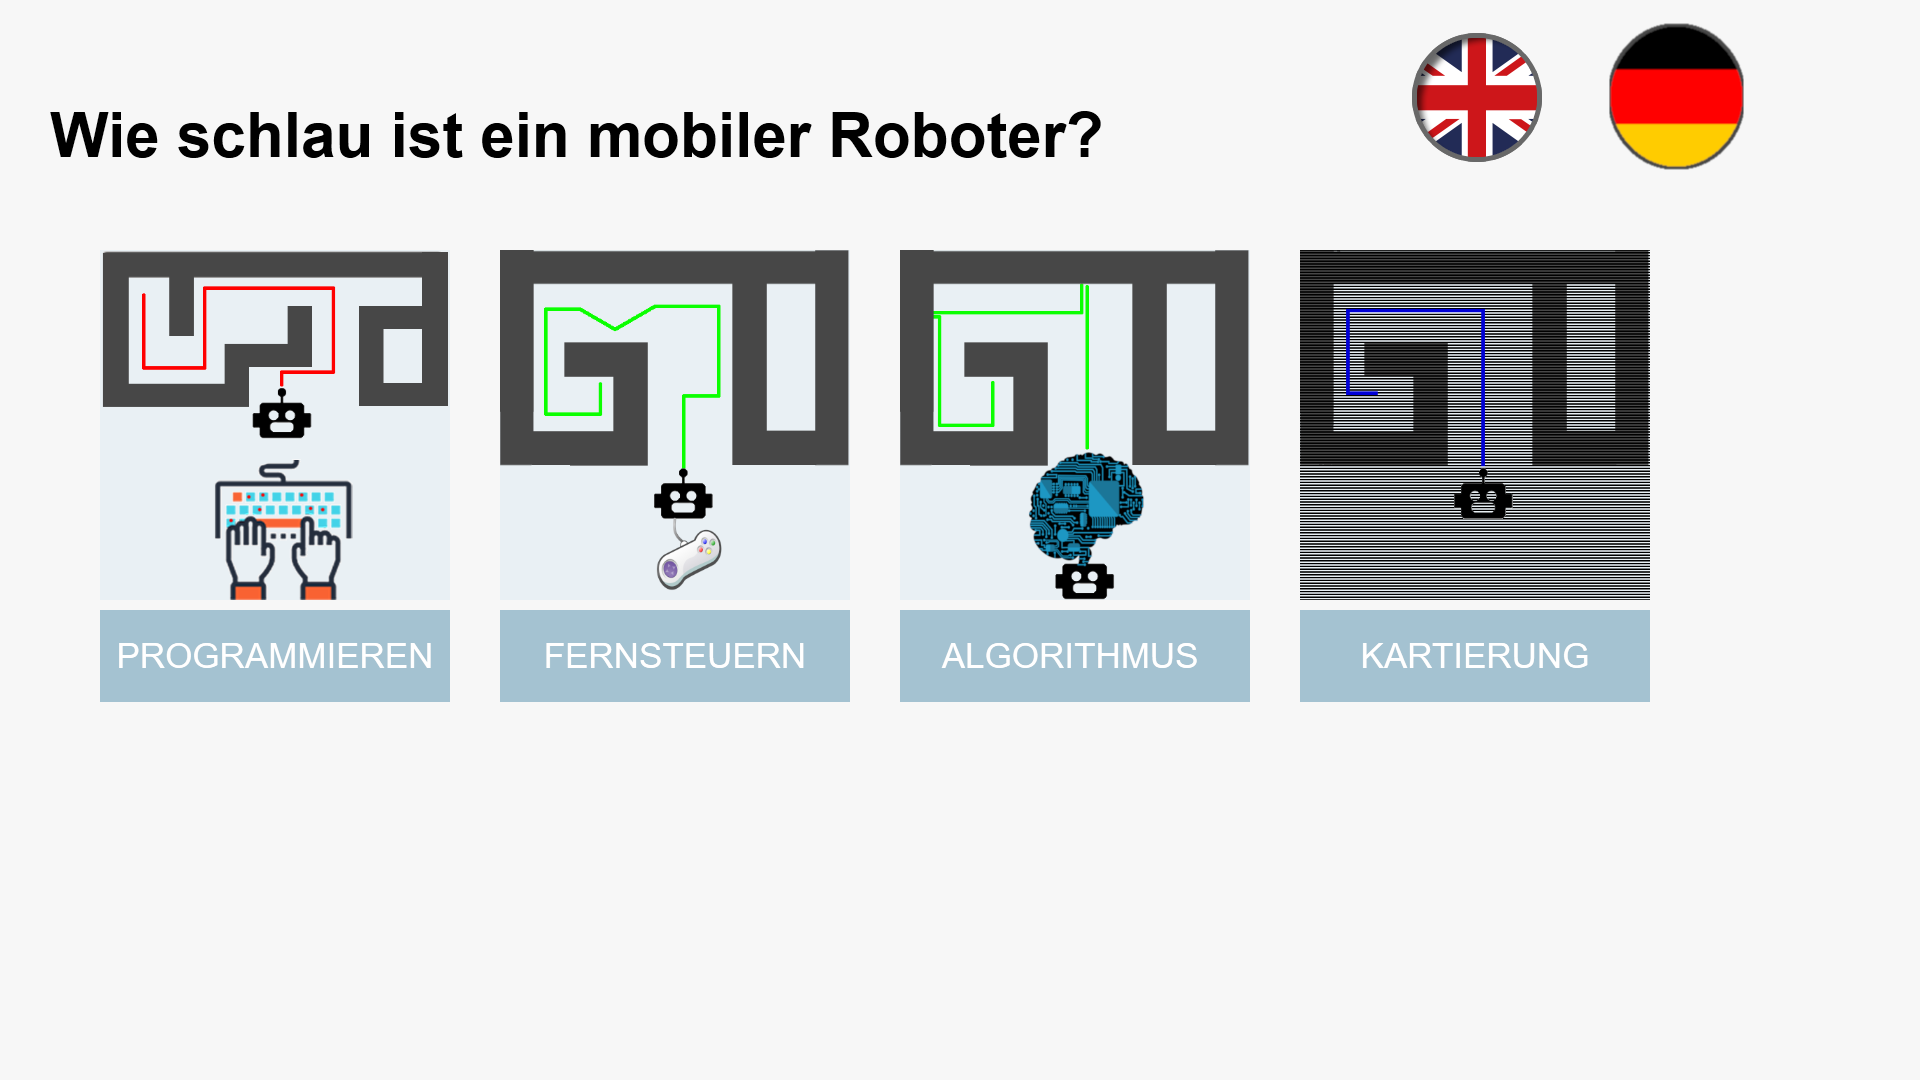
\includegraphics[width=0.5\linewidth]{Bilder/Tests/home_de.PNG}}%
%   \subfloat[][]{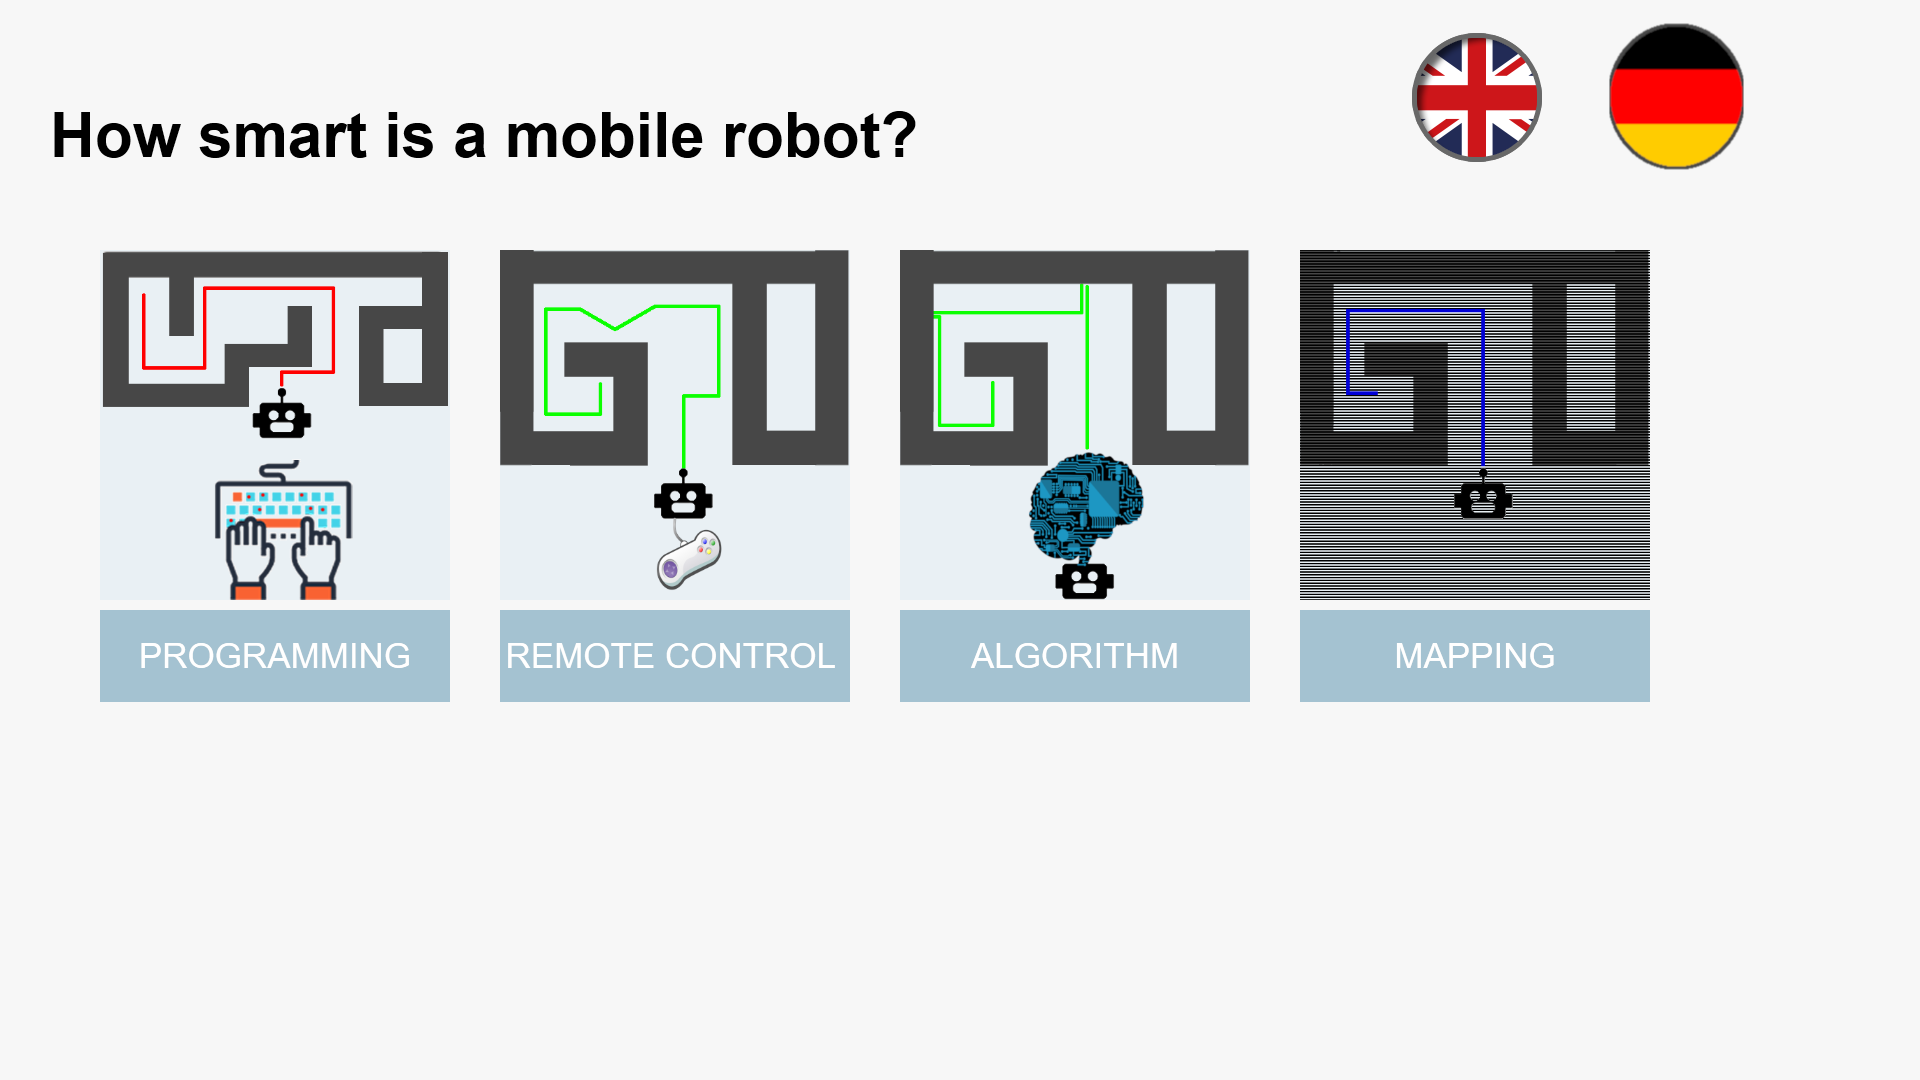
\includegraphics[width=0.5\linewidth]{Bilder/Tests/home_en.PNG}}%
%   \qquad
% %   \subfloat[][]{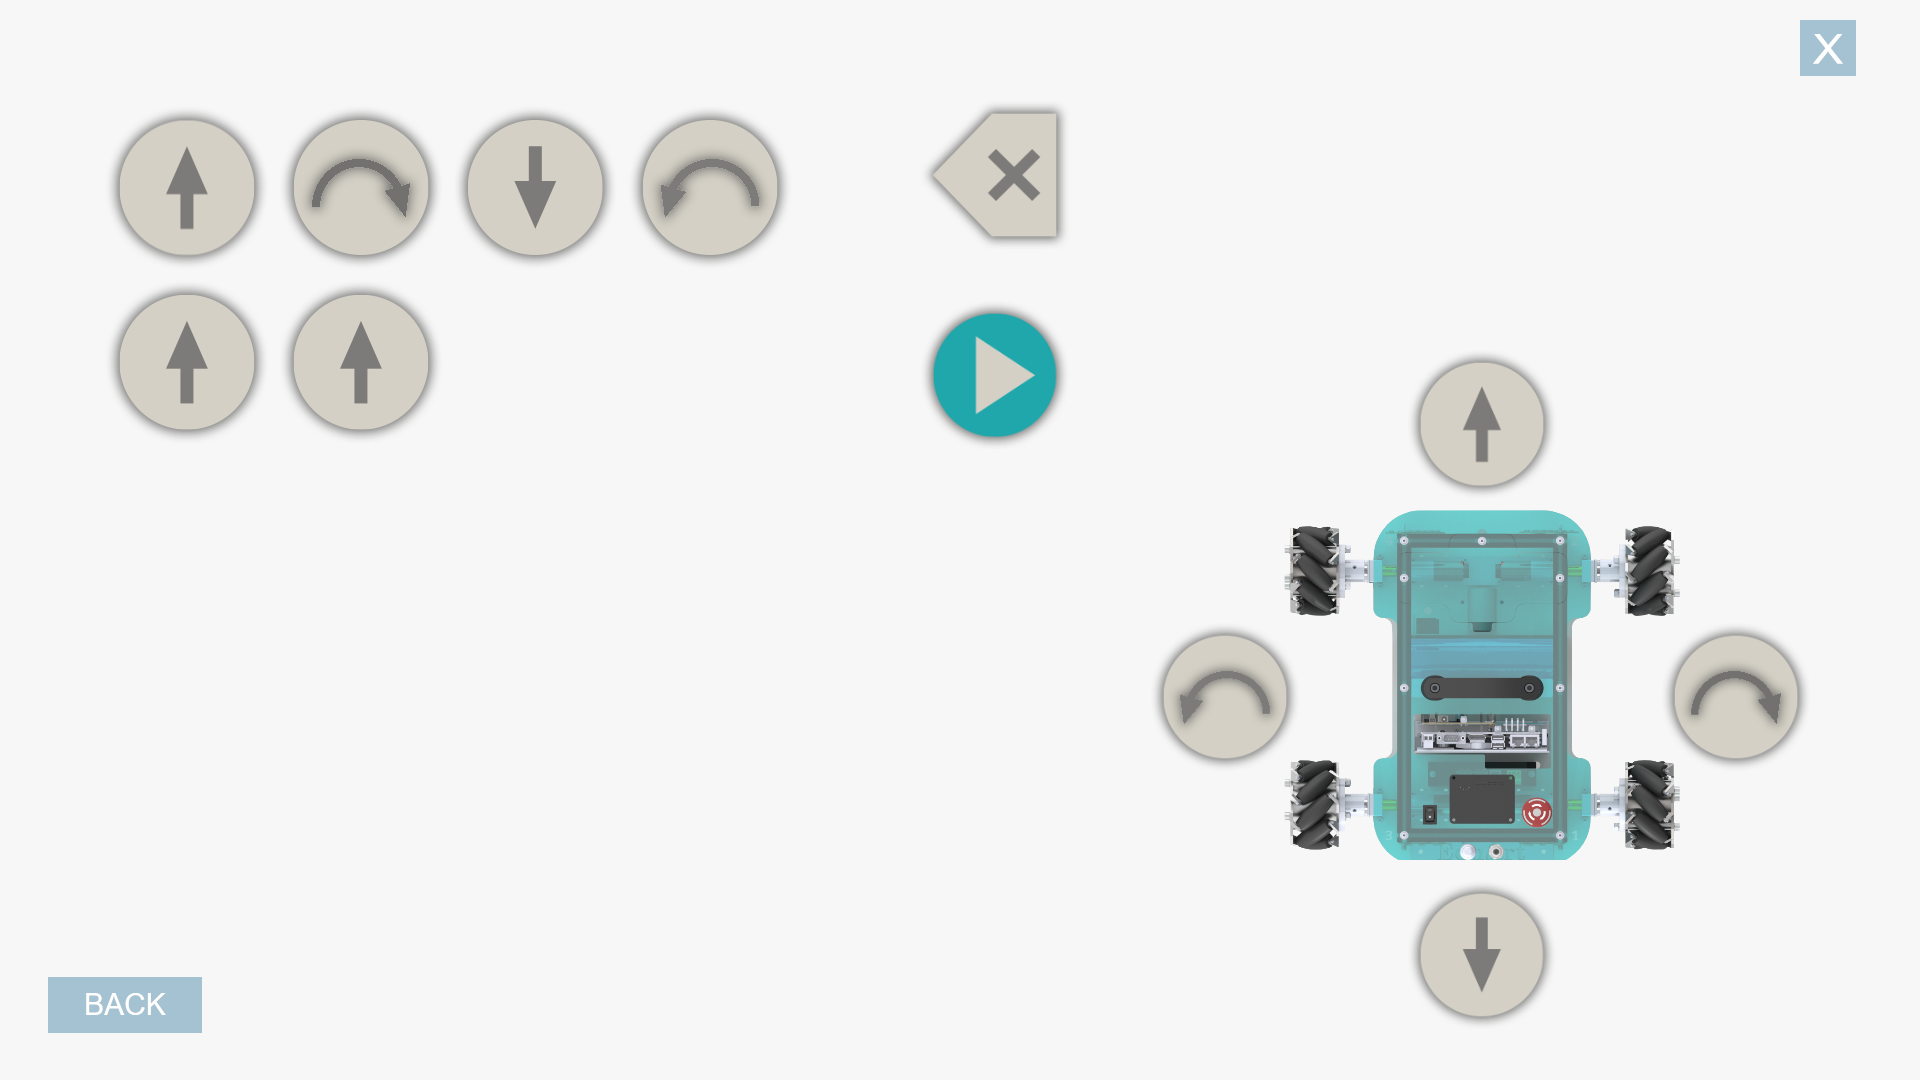
\includegraphics[width=0.5\linewidth]{Bilder/Tests/programming.PNG}}%
% %   \subfloat[][]{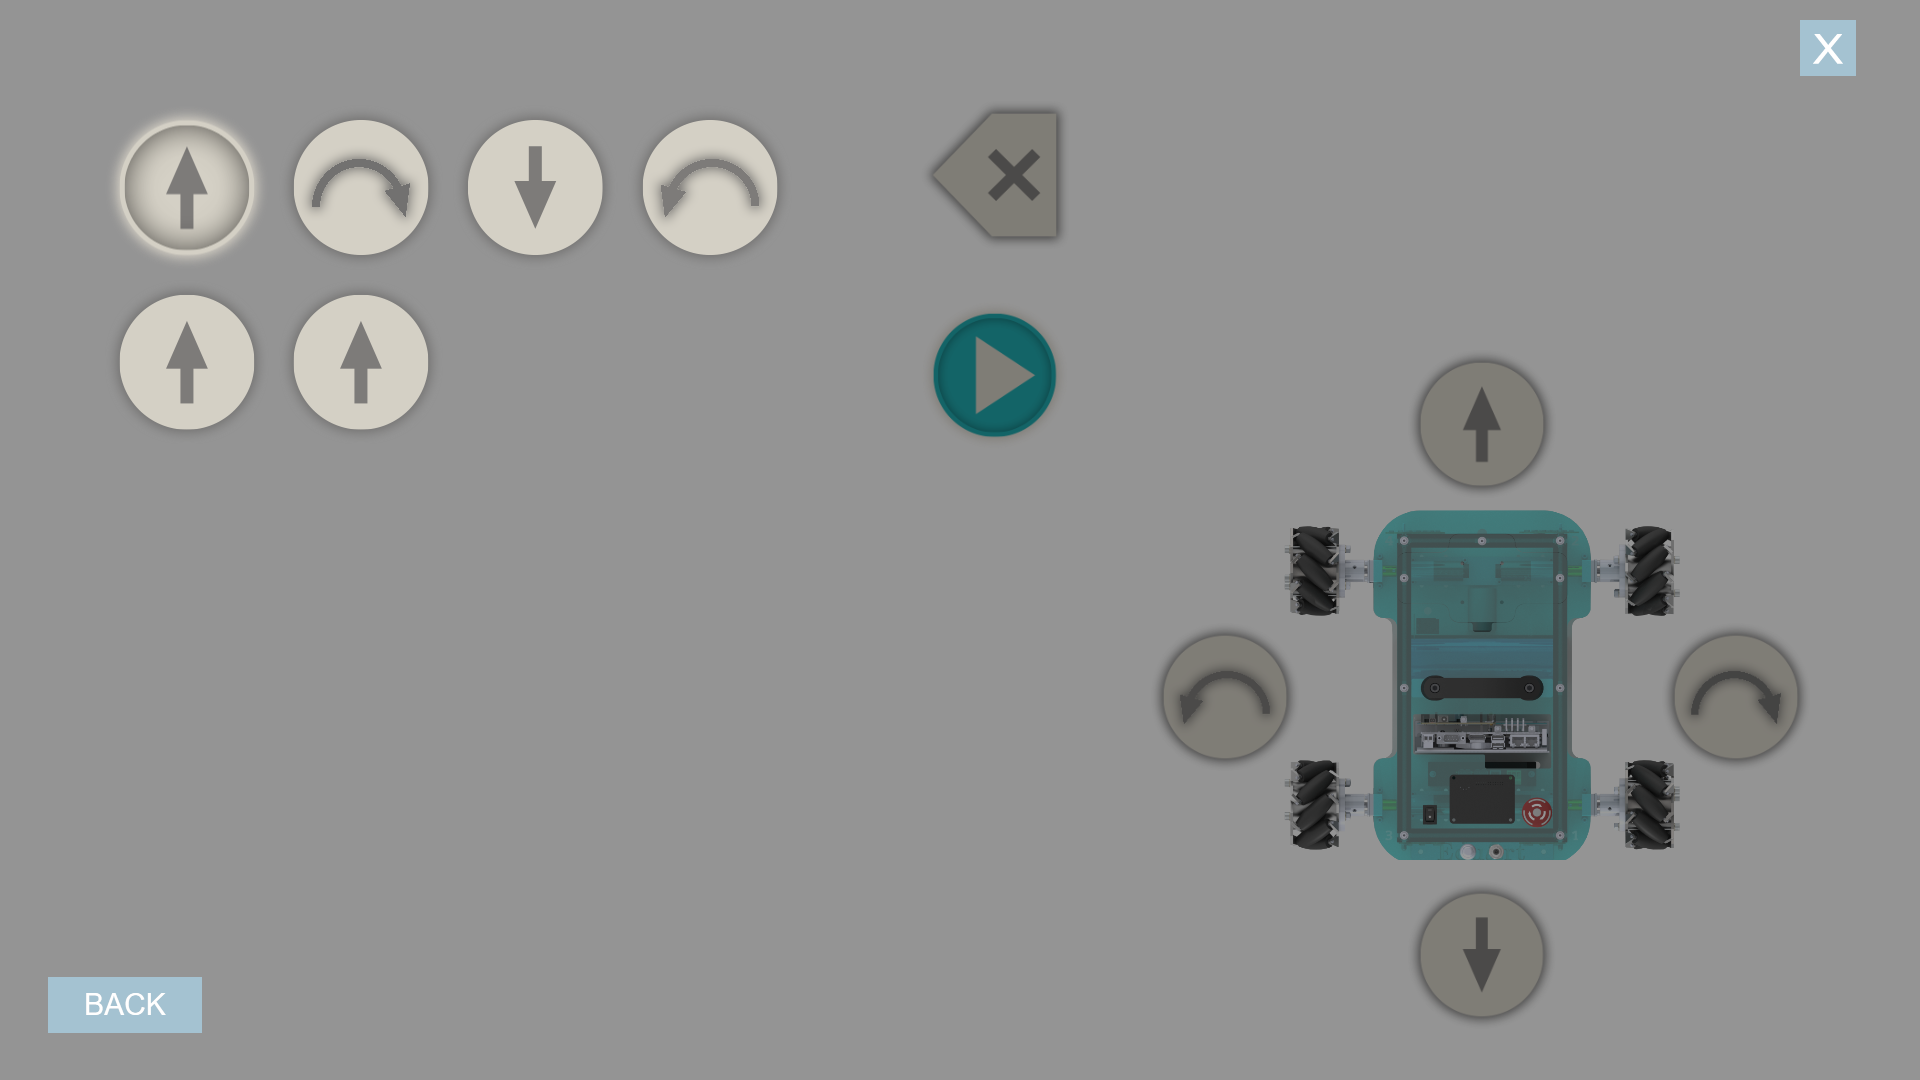
\includegraphics[width=0.5\linewidth]{Bilder/Tests/programming_aktive.PNG}}%
% %   \qquad
%   \subfloat[][]{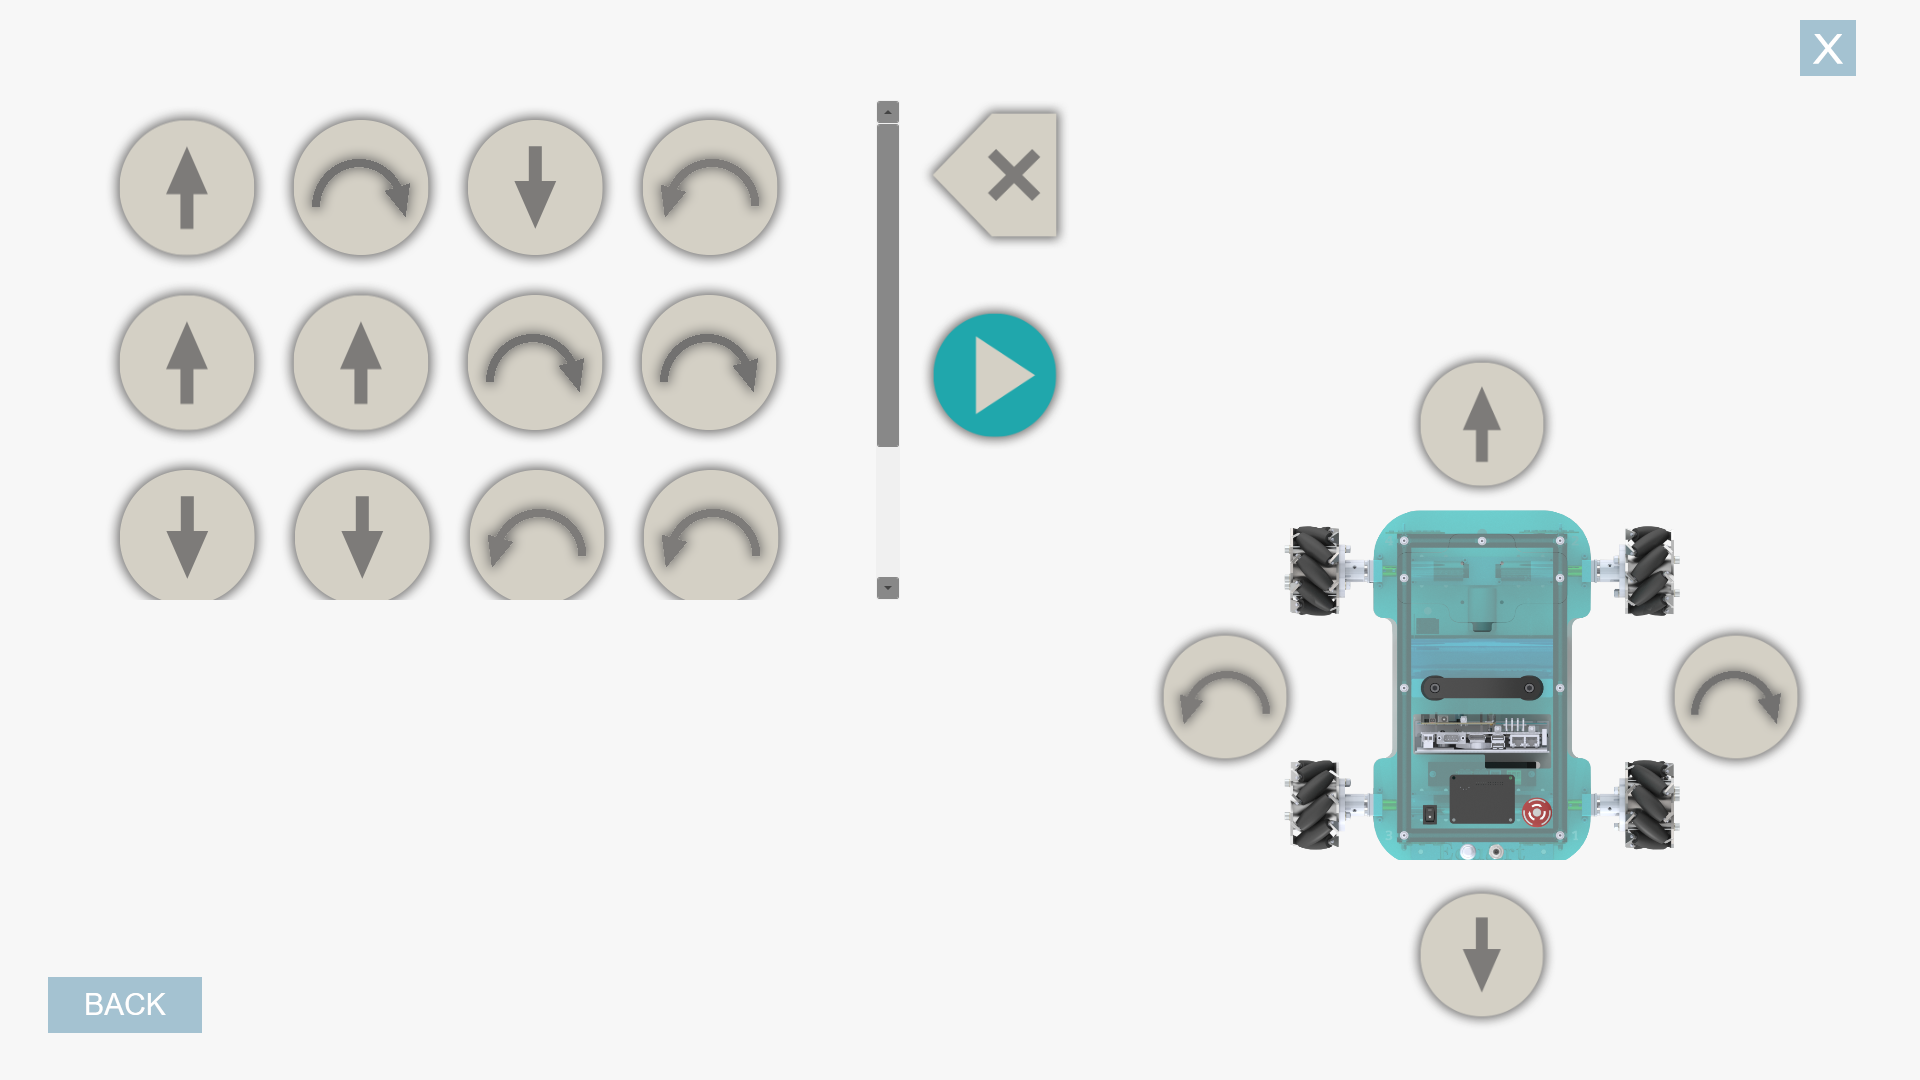
\includegraphics[width=0.5\linewidth]{Bilder/Tests/programming_scroll_scroll.PNG}}%
%   \subfloat[][]{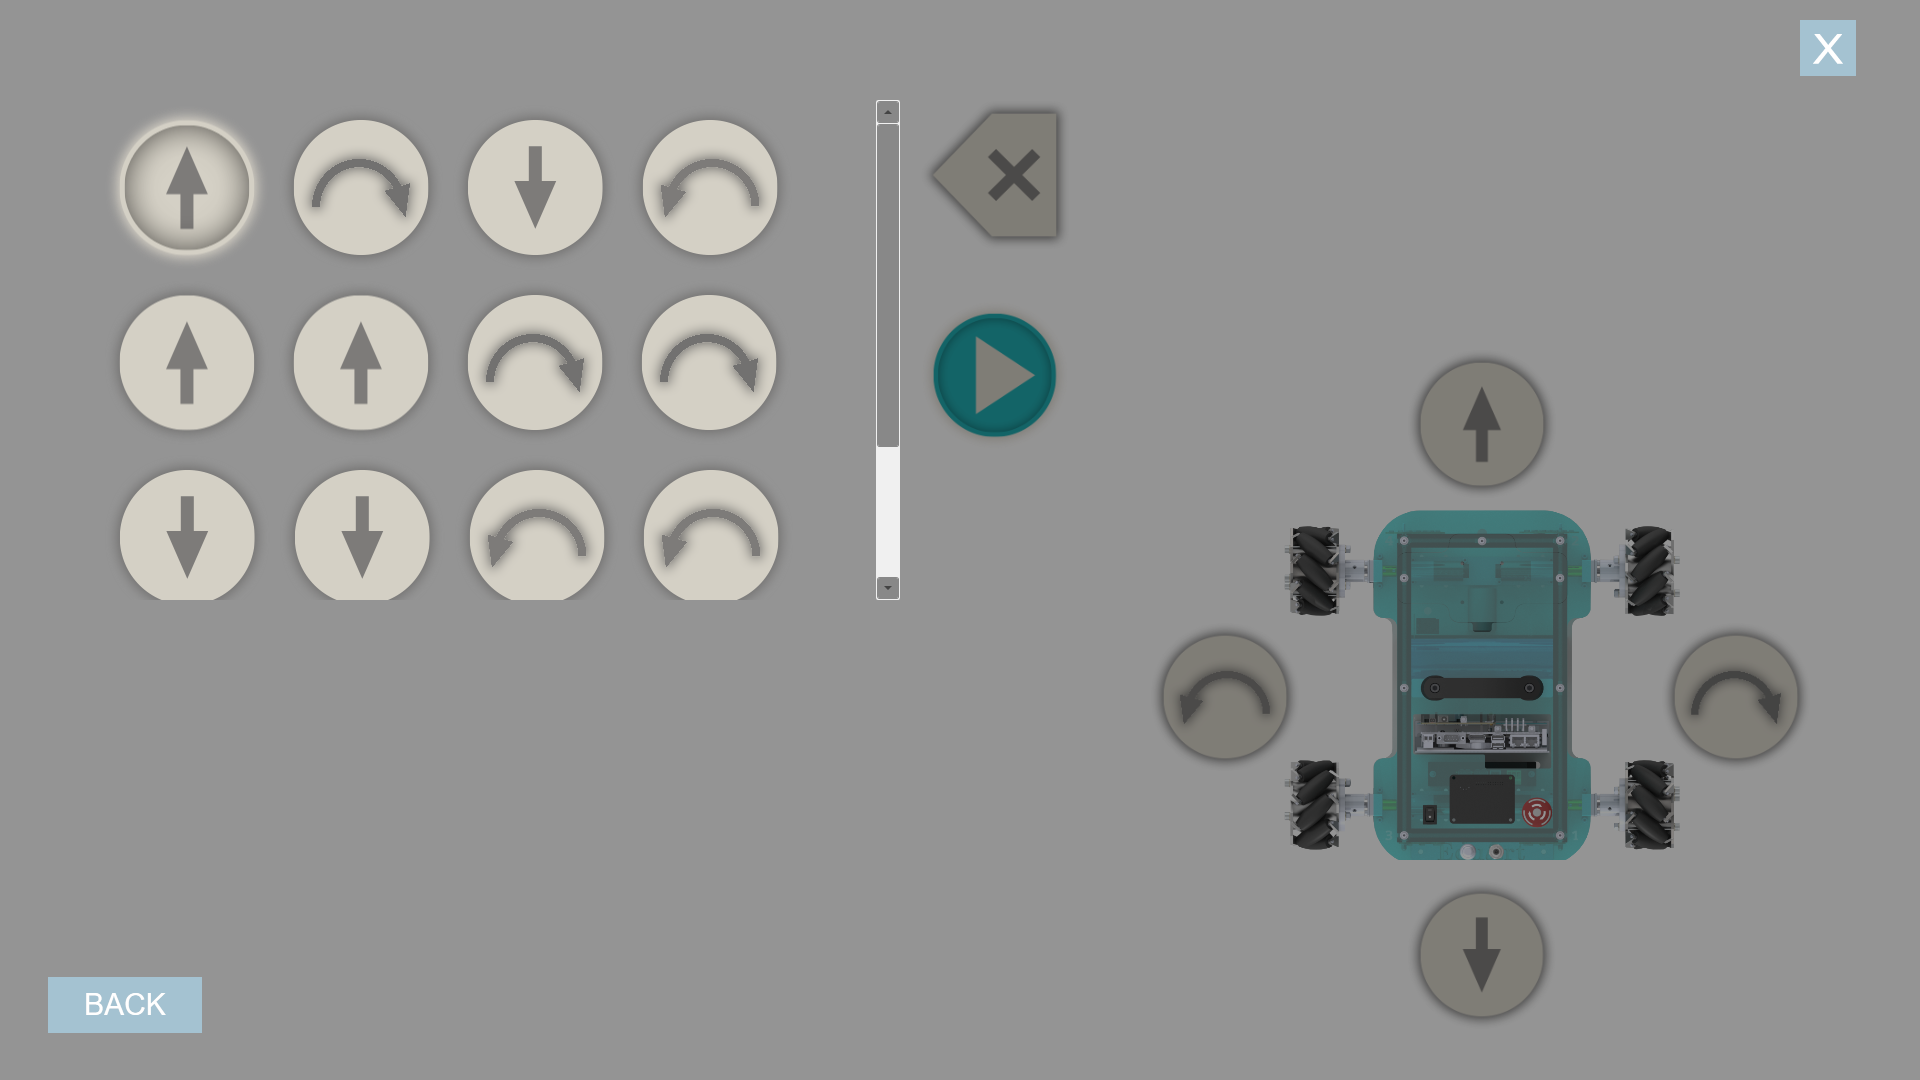
\includegraphics[width=0.5\linewidth]{Bilder/Tests/programming_aktive_scroll.PNG}}%
%   \qquad
  \subfloat[][]{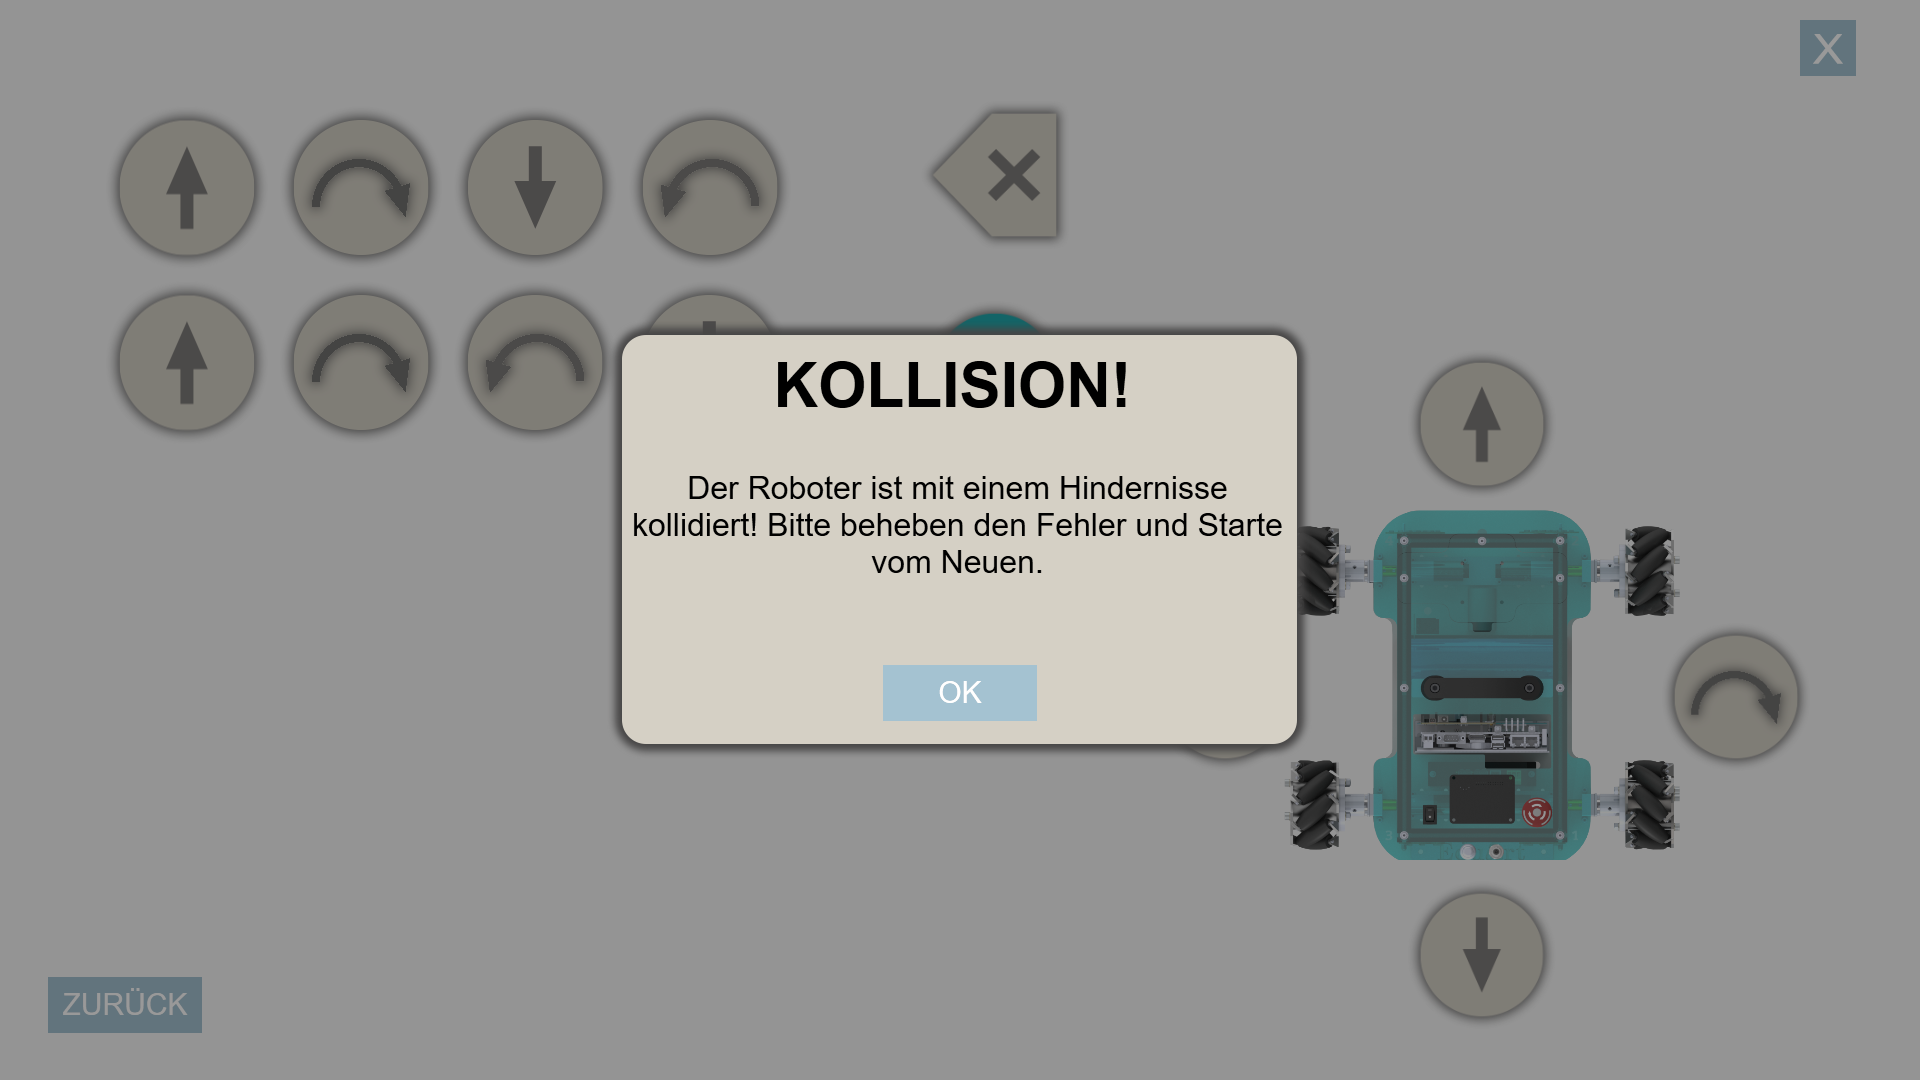
\includegraphics[width=0.5\linewidth]{Bilder/Tests/kollision_de.PNG}}%
  \subfloat[][]{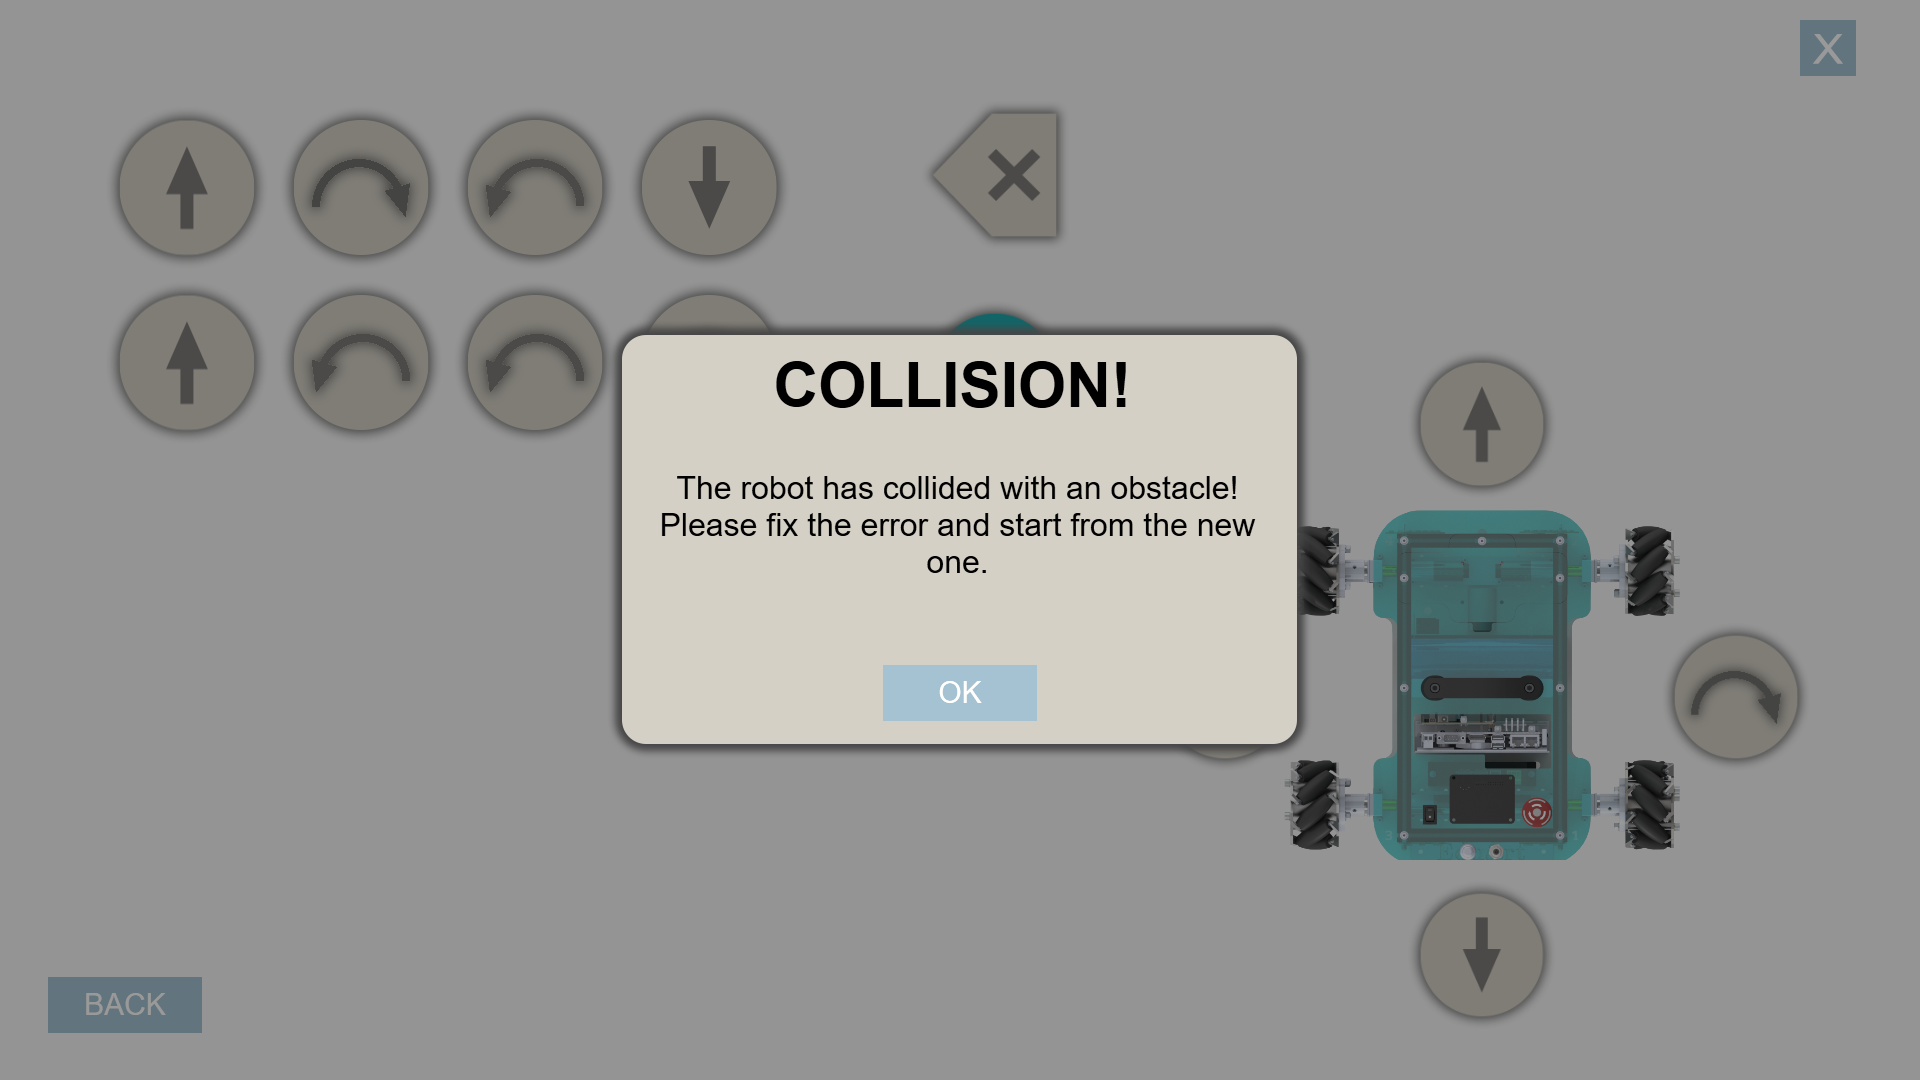
\includegraphics[width=0.5\linewidth]{Bilder/Tests/kollision_en.PNG}}%
  \qquad
  \subfloat[][]{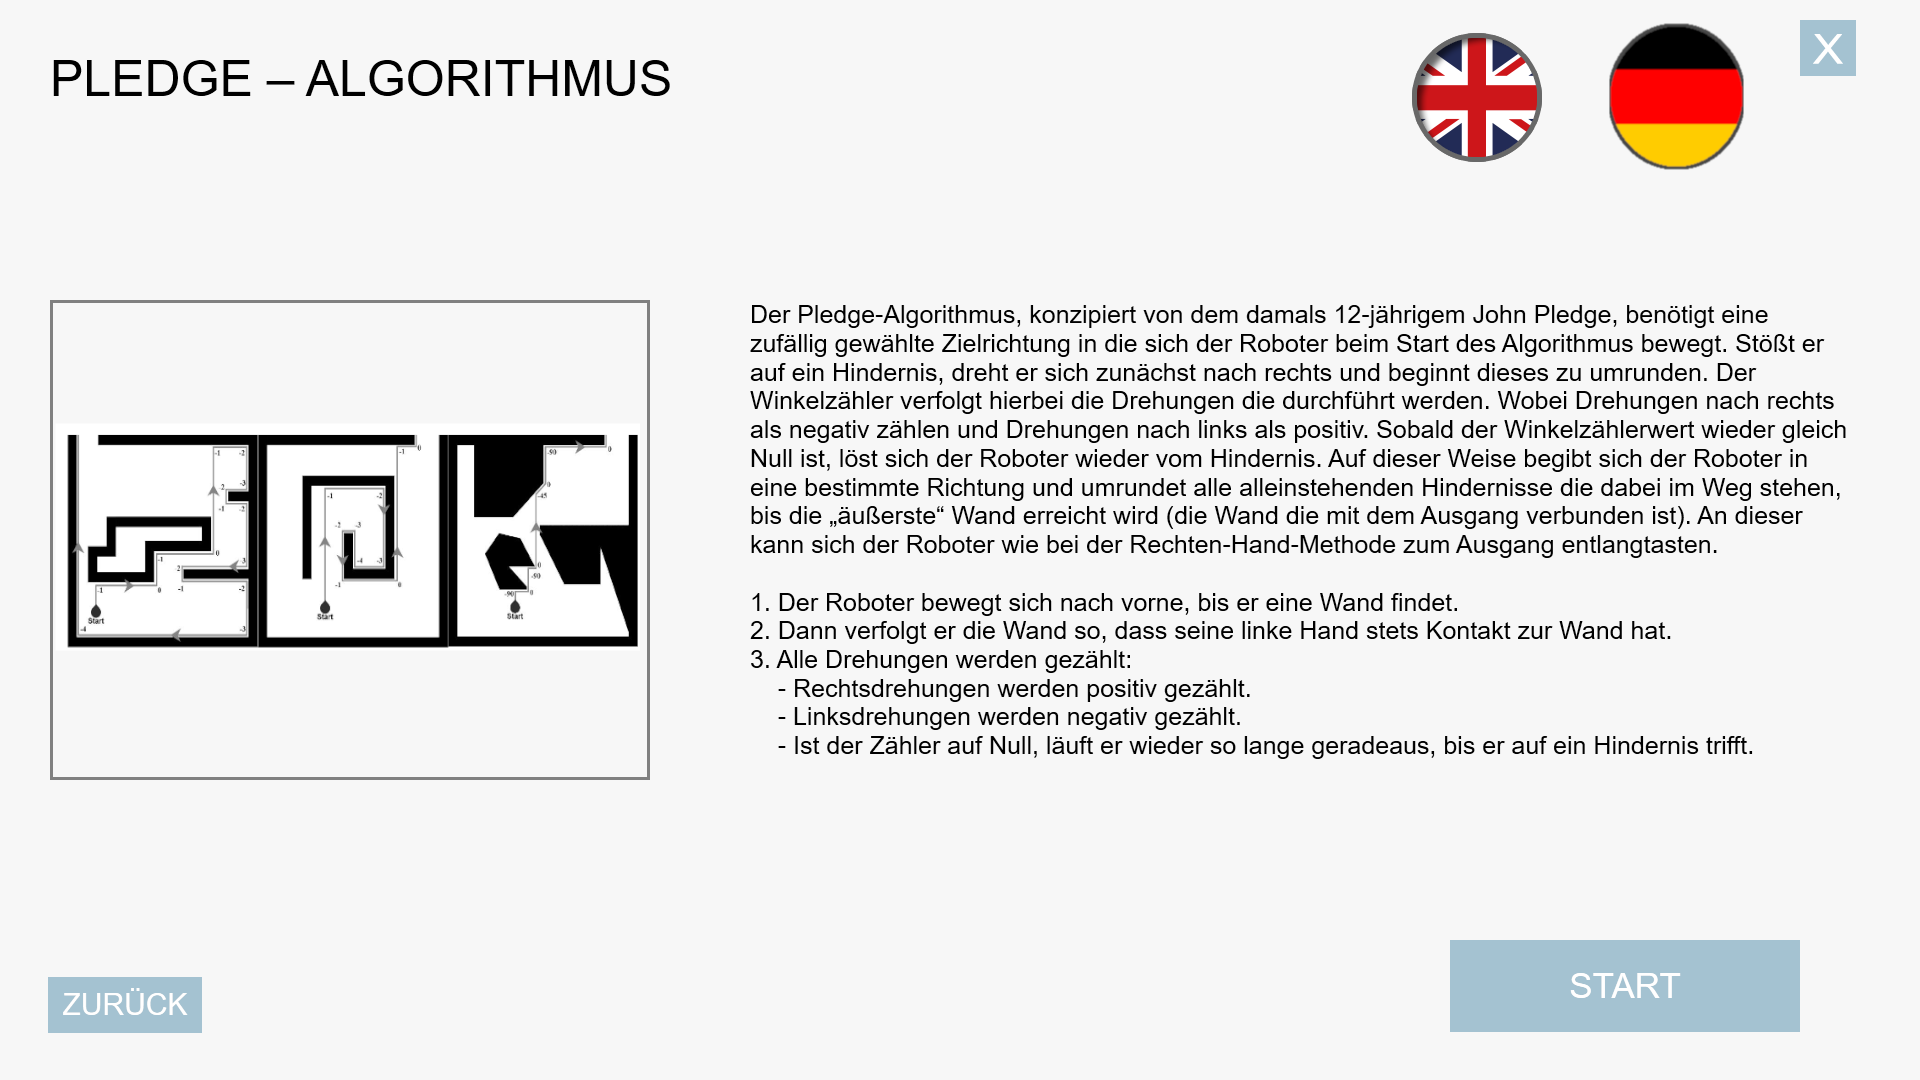
\includegraphics[width=0.5\linewidth]{Bilder/Tests/pledge_de.PNG}}%
  \subfloat[][]{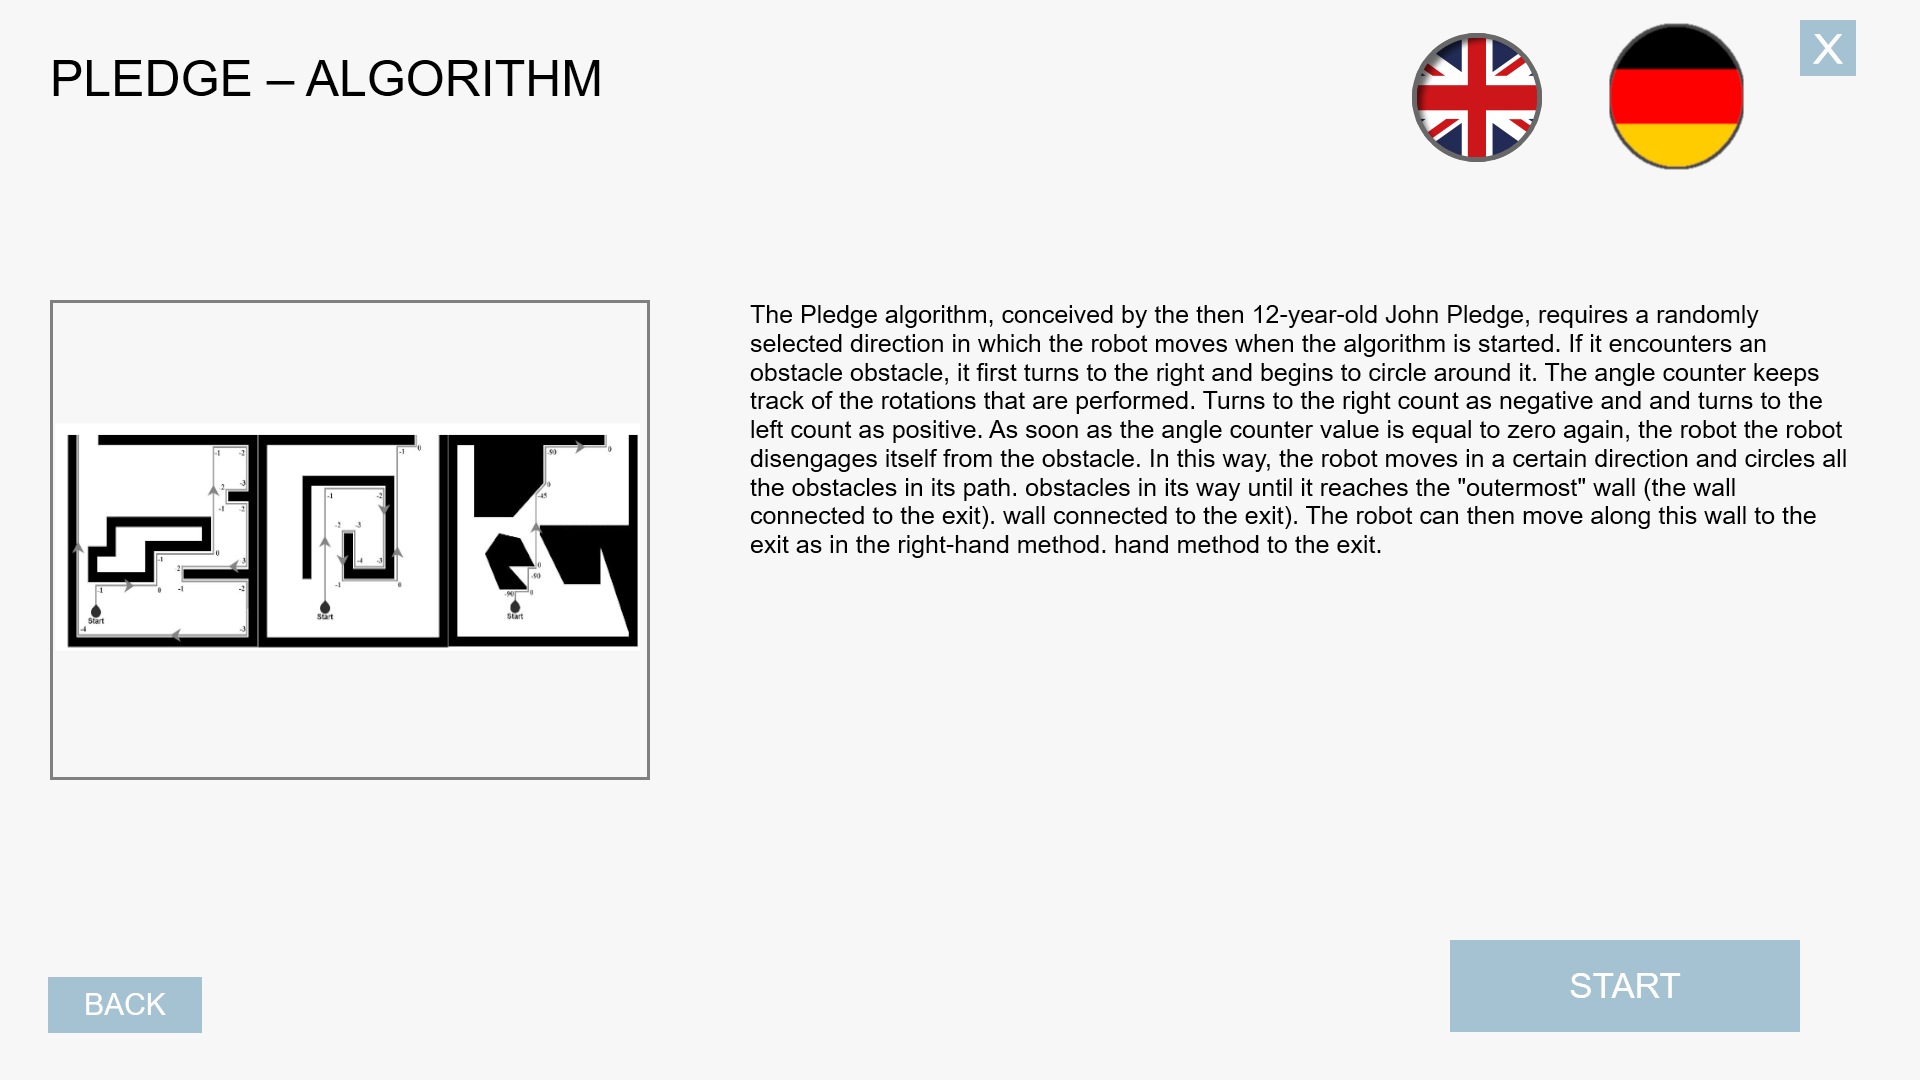
\includegraphics[width=0.5\linewidth]{Bilder/Tests/pledge_en.PNG}}%
  \caption{Test Benutzeroberfläche}
  \label{fig:GUI}
\end{figure}


% \begin{figure}[H]
%  \centering
%  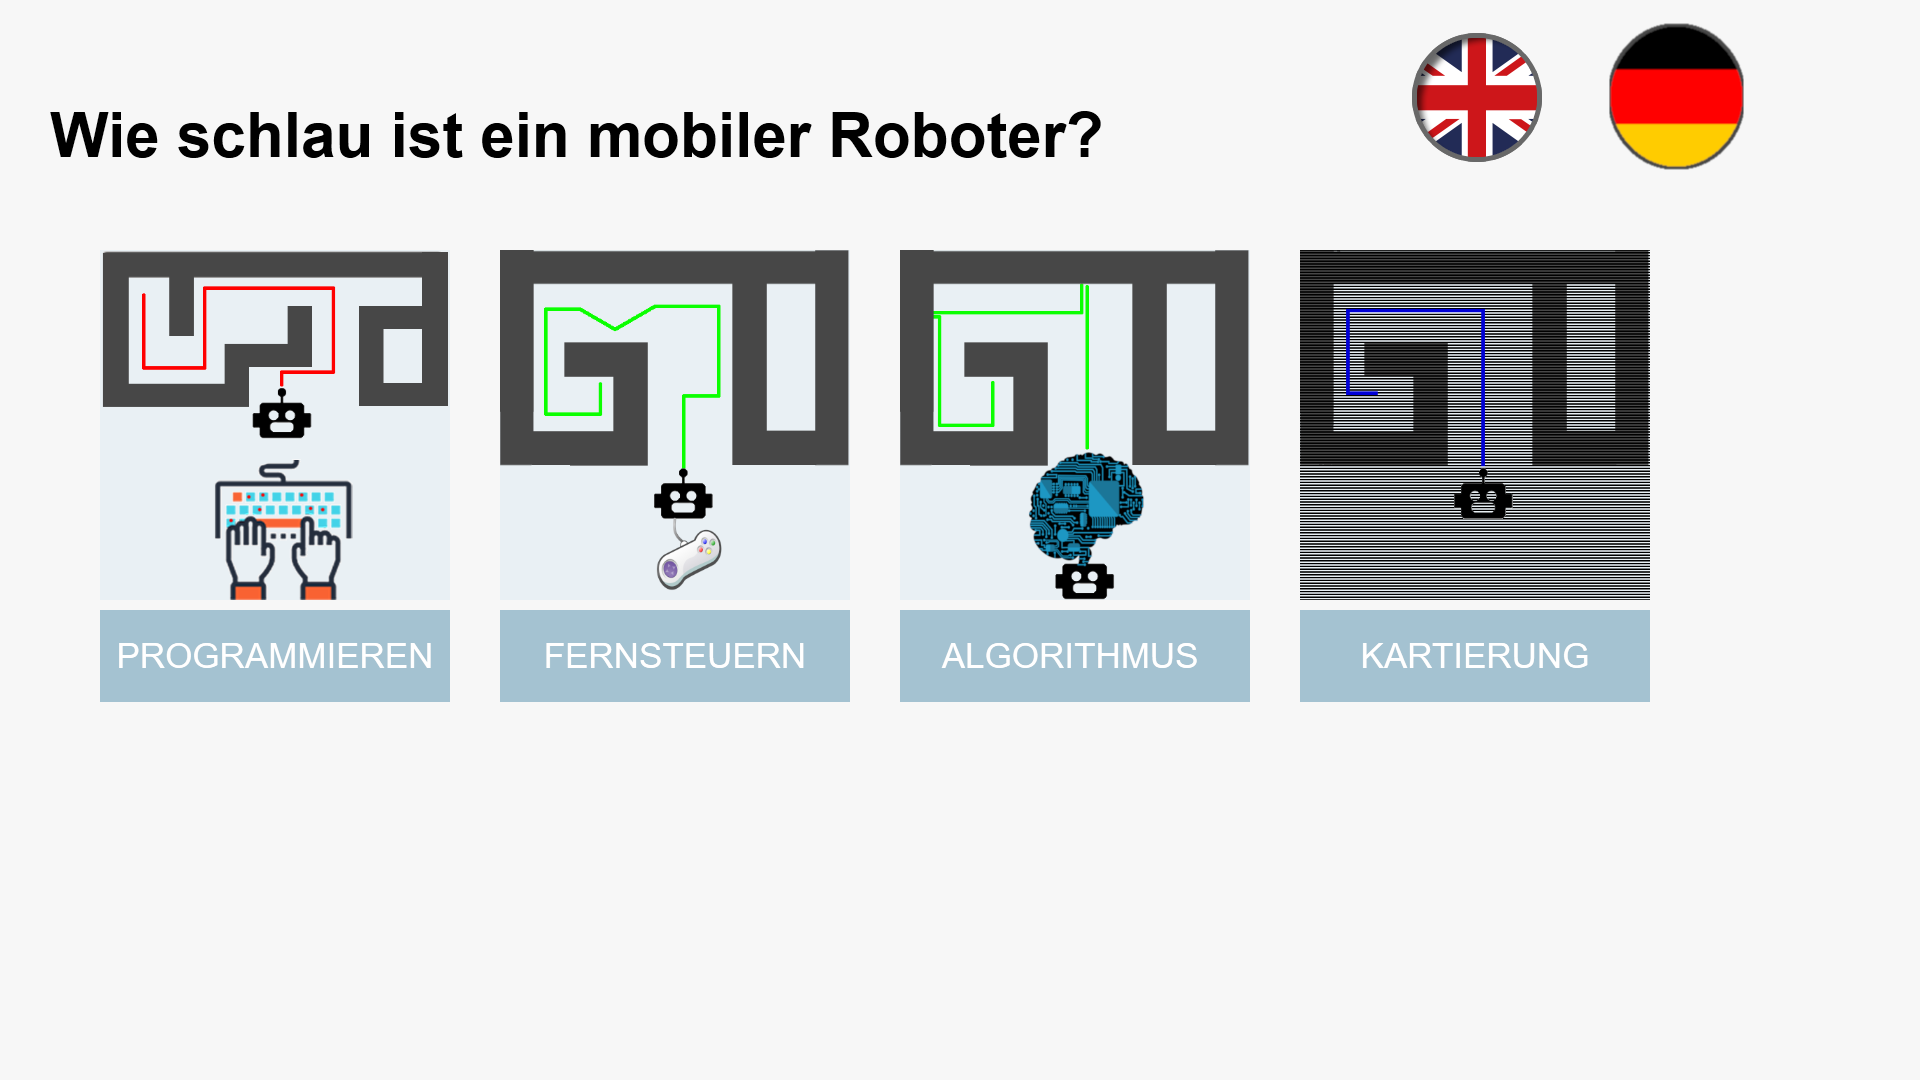
\includegraphics[width=\linewidth]{Bilder/Tests/home_de.PNG}
%  \caption{GUI}
%  \label{fig:GUI}
% \end{figure}


\chapter{Zusammenfassung und Ausblick}
In dieser Arbeit sollte ein System entwickelt werden, das eine Schnittstelle zwischen der Anwendung und der Roboterkontrollarchitektur implementiert (siehe \autoref{fig:gui_puzzel}). 

 \begin{figure}[H]
 \centering
 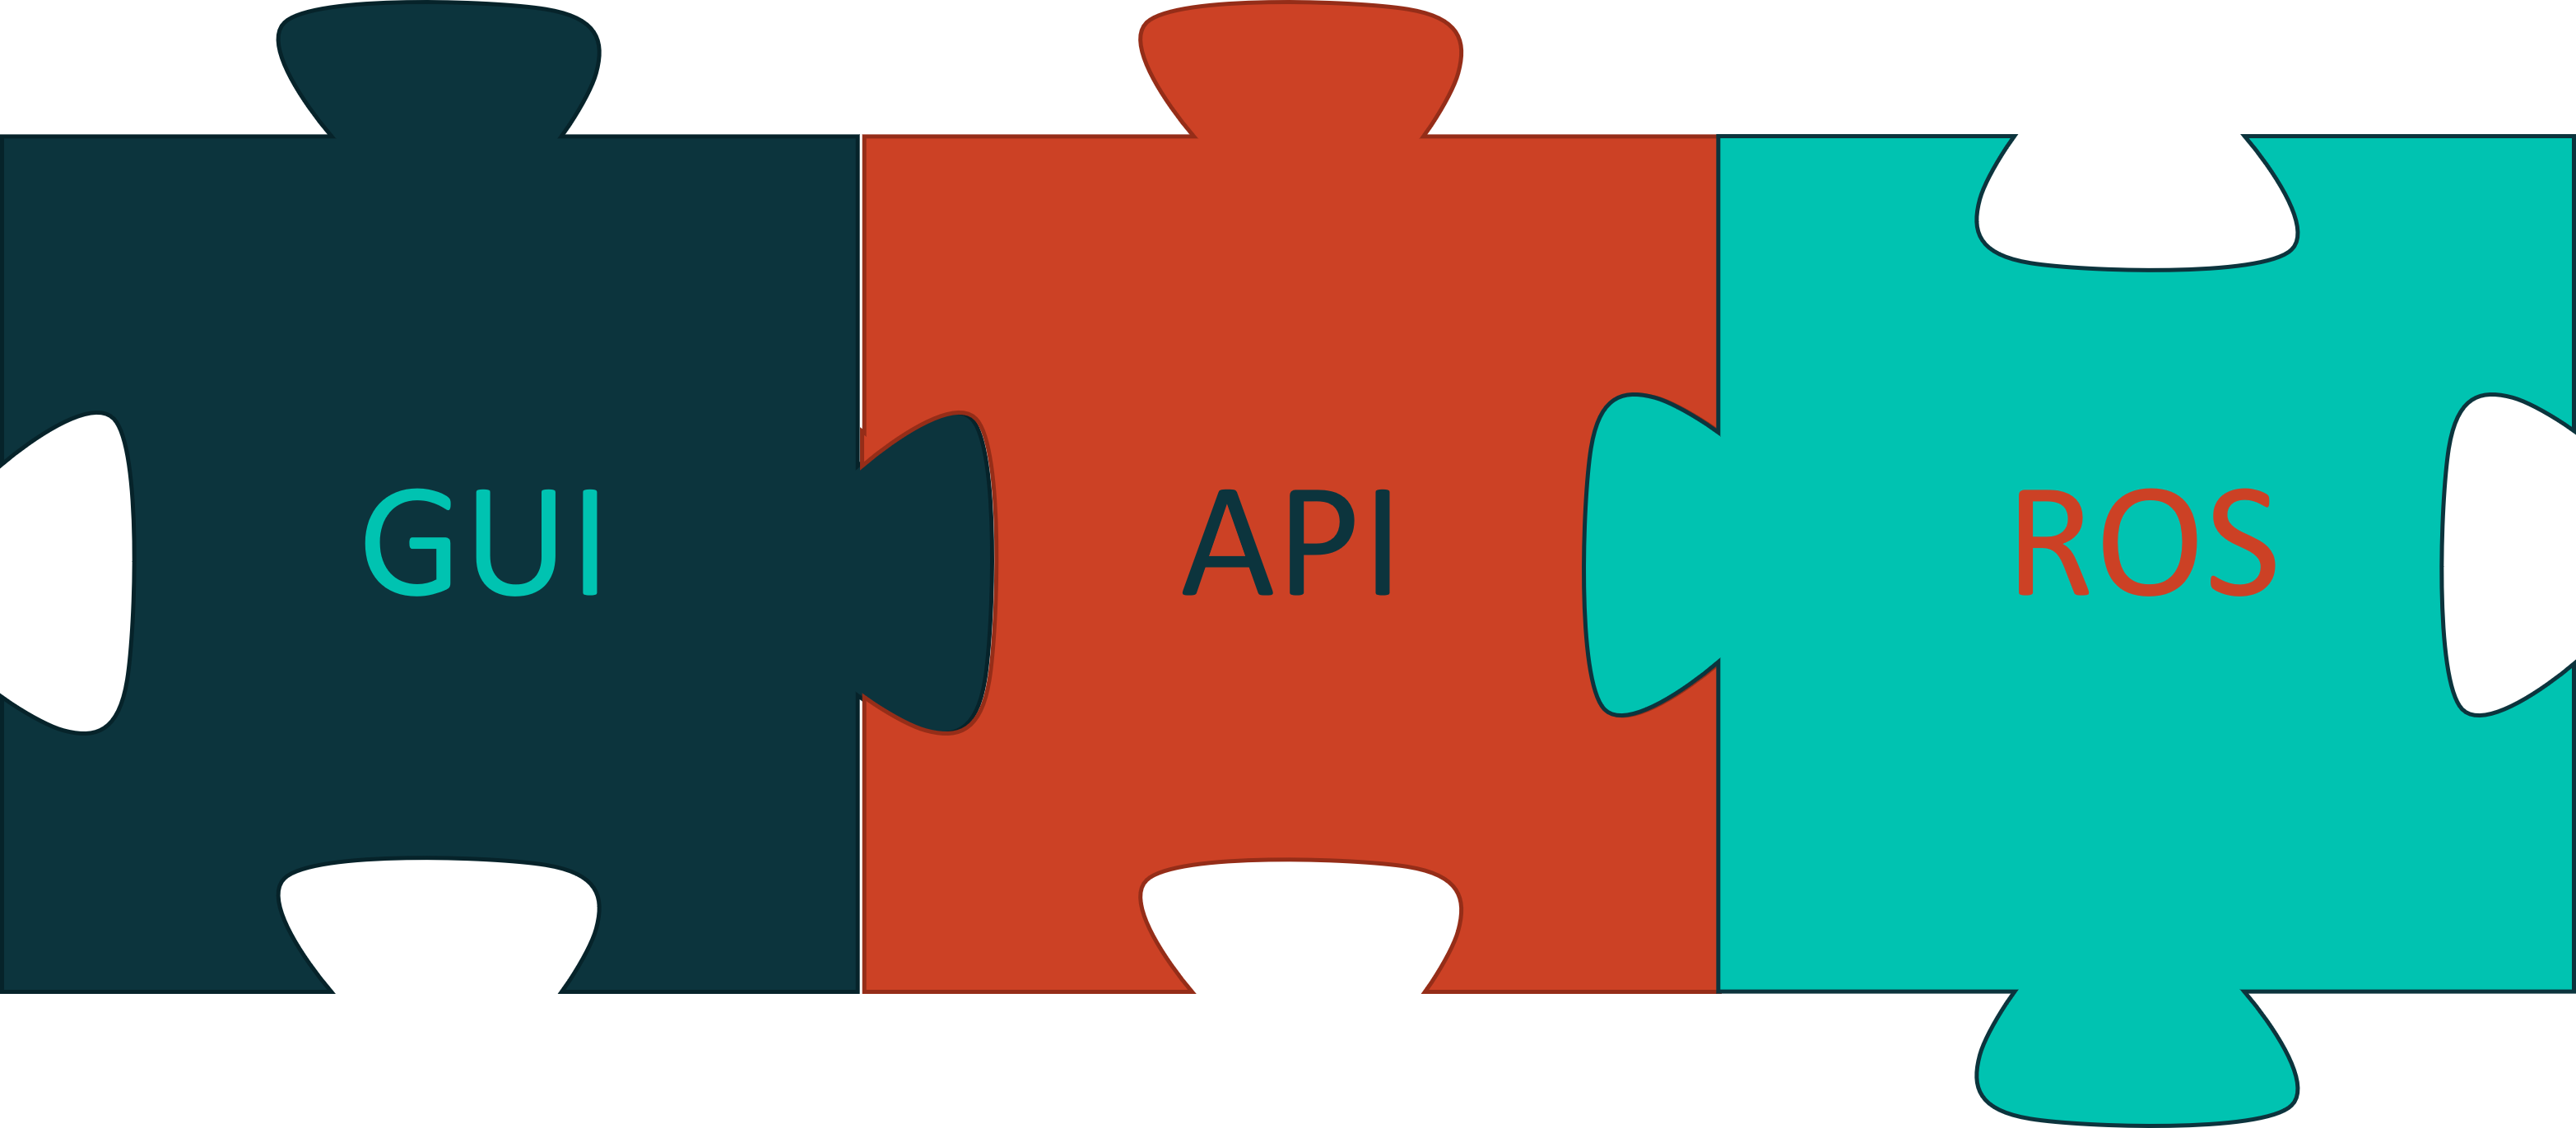
\includegraphics[width=\linewidth]{Bilder/Ausblick/api_bridge.png}
 \caption{Darstellung der Schnittstelle}
 \label{fig:gui_puzzel}
\end{figure}

Dabei sollte das System als ein Exponat vermarktet werden. Der Markt dafür sind Bildungseinrichtungen. So soll spielerisch die Intelligenz von mobilen Robotern vermittelt werden. Ein weiterer Einsatzbereich ist die Vermittlung von Informationstechnologie. So kann die Benutzeroberfläche als Lehrmaterial gestaltet werden, um Schüler und Studierenden das Programmieren oder das technische Denken spielerisch zu transportieren. Dies würde somit die alteingesessenen Methoden mit Büchern oder Simulationen ergänzen. Das System in dieser Arbeit verwendet verschiedene Sensoren, die im Laufe des Projektes immer wieder ergänzt wurden, um mehrere Möglichkeiten abzudecken. So konnte mithilfe eines rotierenden Laserscanners der Abstand zu Hindernissen gemessen werden und im Programm die Hindernisse vermieden werden. Dies ermöglichte auch eine relative Navigation des mobilen Roboters. Des Weiteren wurden Ultraschallsensoren seitlich des Roboters integriert, um dem Pledge- Algorithmus ausreichende Daten zu liefern. Dazu wurde eine separate Implementierung vorgenommen, um den Sensor abzufragen und über ROS die Werte zu veröffentlichen. Die Fähigkeiten von mobilen Robotern sollten mithilfe des Befreiungsalgorithmus im Labyrinth aufgezeigt werden. Dazu wurde der Plegde- Algorithmus verwendet, der auch schon bewiesen hatte, dass er immer einen Ausweg findet, wenn ein Ausweg aus dem Labyrinth existiert. Das Ganze wurde nur prototypisch als Zustandsautomat entwickelt und nur einzelne Teile wurden getestet. Im kompletten zusammenhängenden Ausmaß wurden dazu keine Tests durchgeführt. Die Arbeit entstand in der Zusammenarbeit mit der Firma Kurt Hüttinger GmbH und somit sollte das System als ein komplettes Exponat vermarktet werden. So war bei der Entwicklung klar, dass es keinen wirklichen Ausweg aus dem Labyrinth geben wird. Um trotzdem ein Ziel zu definieren, wurde das System mit einer Kamera erweitert, damit durch QR-Codes das Ziel markiert werden kann. Diesbezüglich wurde ein separates Modul entwickelt, das mithilfe von ZBar, QR-Codes aus Livebilddaten ausliest und über ROS veröffentlicht. Dadurch kann das Ende für den Algorithmus detektiert werden. Das Bindeglied der ganzen einzelnen Teile ist das API. Das API verbindet die ganzen Module miteinander und ermöglich durch Standard-Netzwerkprotokolle die Bedienung des mobilen Roboters.\\
Das ganze System wurde an die Firma Kurt Hüttinger GmbH \& Co. KG übergeben. Die Schnittstelle kann so eingesetzt werden. Die Firma kann das System mit weiteren Funktionalitäten erweitern, da es bausteinförmig und objektorientiert aufgebaut ist.\\
Dadurch das die Implementierung relativ modular und objektorientiert aufgebaut ist, können leicht weitere Intelligenzen eingebaut werden. So kann als Ausblick genannt werden die Kartierung vom Labyrinth mit SLAM und im Anschluss der Kartierung kann die Navigation mithilfe von weiteren Algorithmen für Pfadfindung erfolgen. Dazu kann der A-Star oder Dijkstra Algorithmus genannt werden, die als Suchalgorithmus dienen. Da auch künstliche Intelligenz immer mehr gefragt und eingesetzt wird, kann dieses System auch mit einer künstlichen Intelligenz erweitert werden, wie zum Beispiel mit einer Kamera, die Objekte und Gegenstände erkennt und je nachdem Entscheidungen trifft. So können auch Rampen eingebaut werden und der mobile Roboter erkennt diese, fährt über die Rampe, wird also diese nicht mehr als Hindernis betrachten. Im Allgemeinen kann das Projekte noch mit vielen Möglichkeiten und Intelligenzen erweitert werden. 
% \input{Abschnitte/Platinenaufbau}
% \input{Abschnitte/Motorregelung}
% \input{Abschnitte/Inbetriebnahme}
% \chapter{Zusammenfassung und Ausblick}
In dieser Arbeit sollte ein System entwickelt werden, das eine Schnittstelle zwischen der Anwendung und der Roboterkontrollarchitektur implementiert (siehe \autoref{fig:gui_puzzel}). 

 \begin{figure}[H]
 \centering
 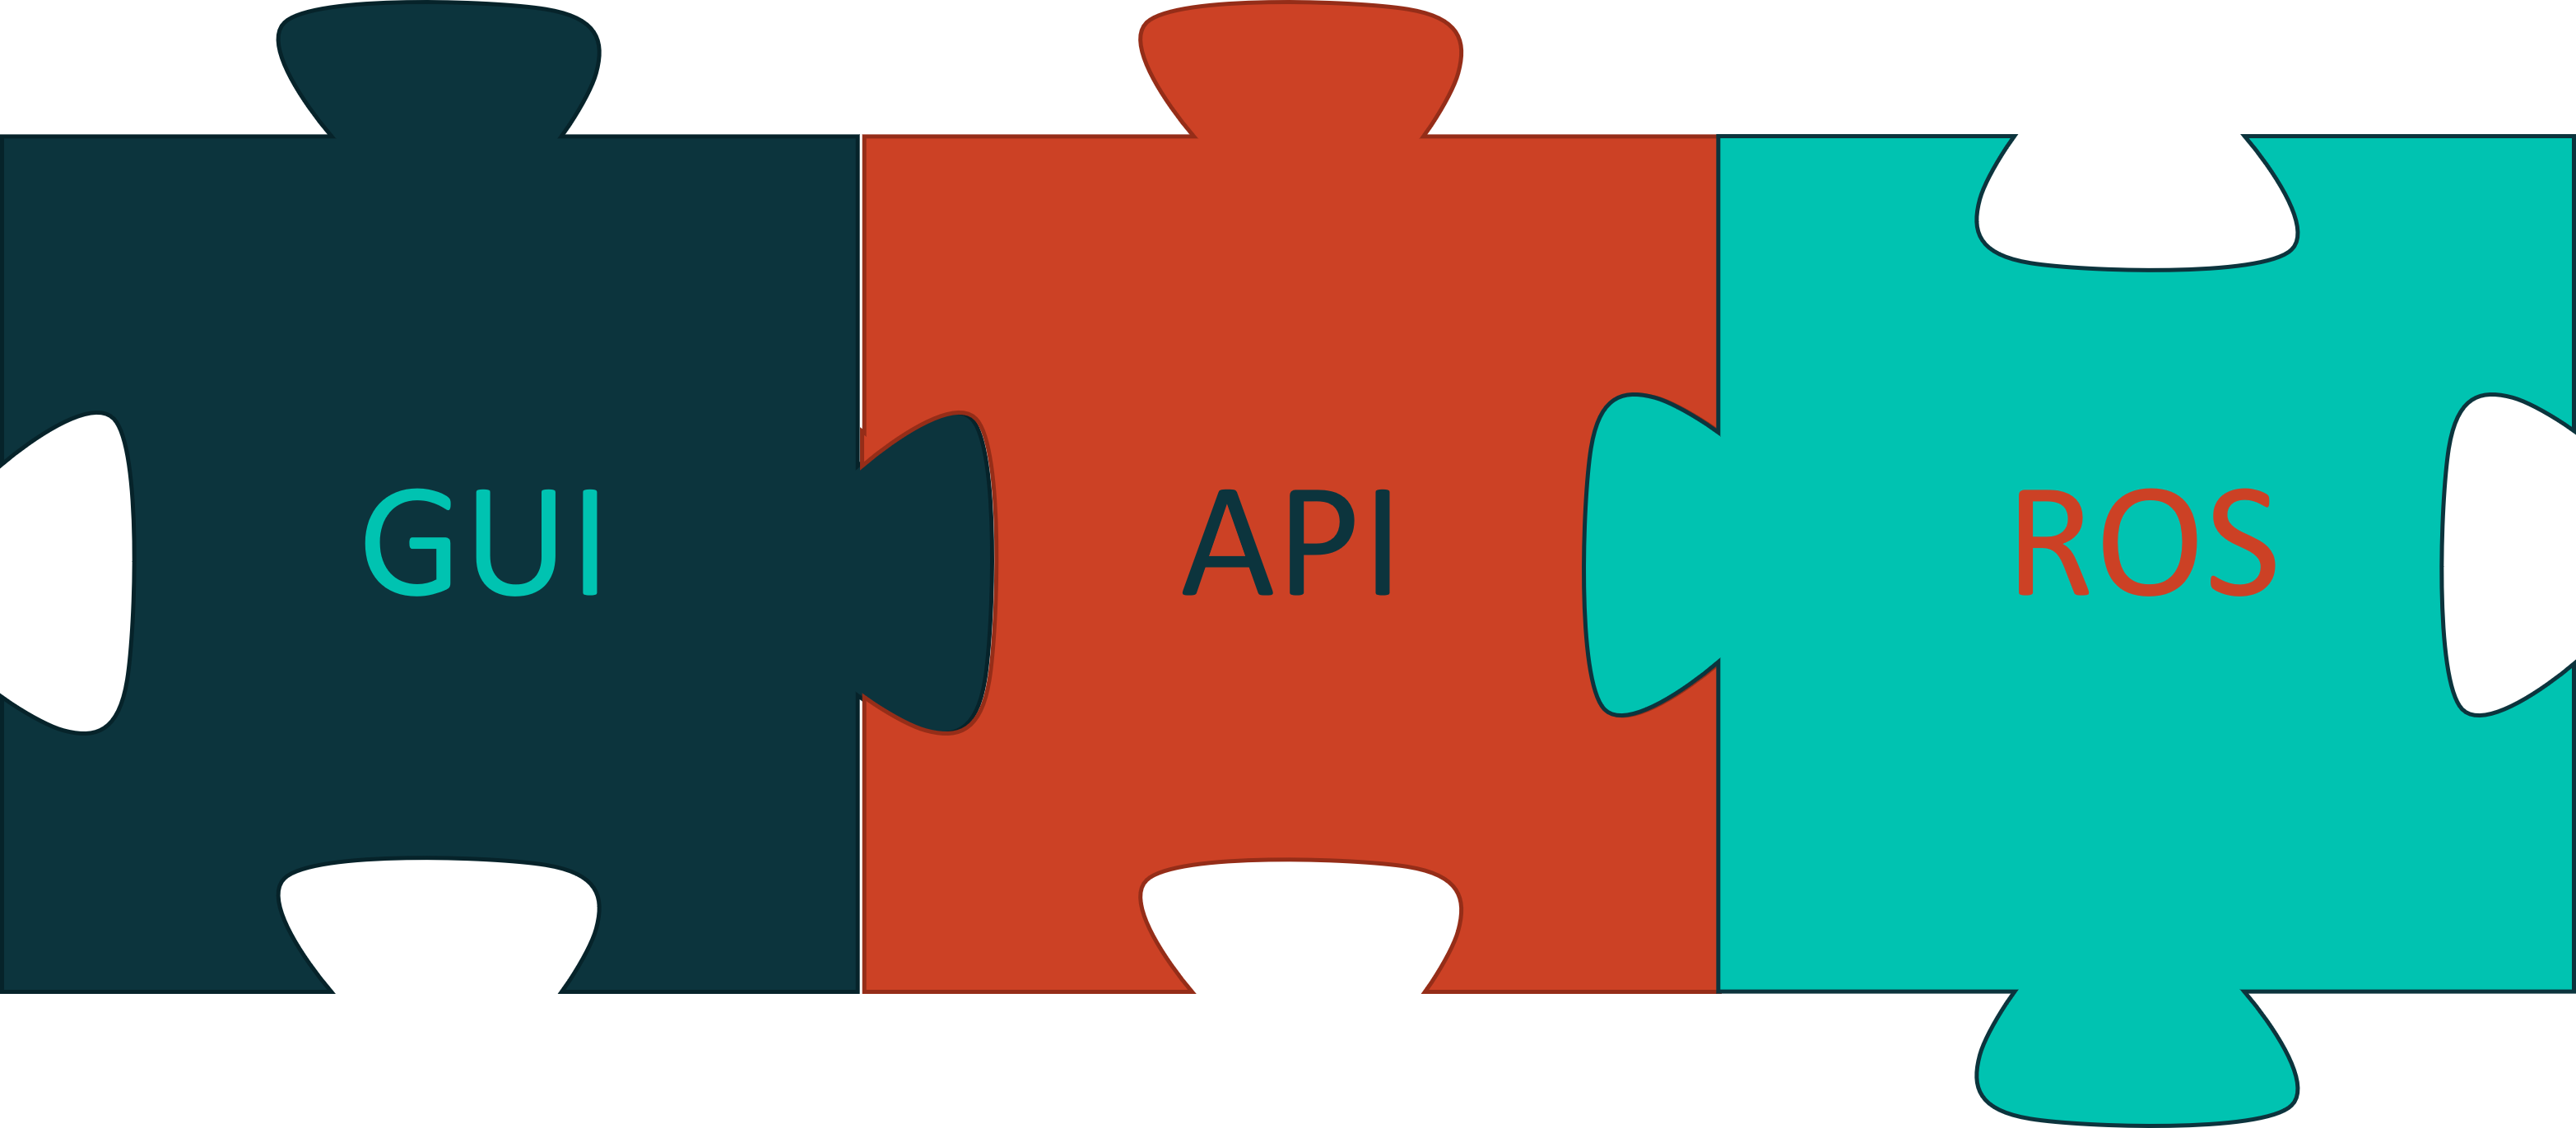
\includegraphics[width=\linewidth]{Bilder/Ausblick/api_bridge.png}
 \caption{Darstellung der Schnittstelle}
 \label{fig:gui_puzzel}
\end{figure}

Dabei sollte das System als ein Exponat vermarktet werden. Der Markt dafür sind Bildungseinrichtungen. So soll spielerisch die Intelligenz von mobilen Robotern vermittelt werden. Ein weiterer Einsatzbereich ist die Vermittlung von Informationstechnologie. So kann die Benutzeroberfläche als Lehrmaterial gestaltet werden, um Schüler und Studierenden das Programmieren oder das technische Denken spielerisch zu transportieren. Dies würde somit die alteingesessenen Methoden mit Büchern oder Simulationen ergänzen. Das System in dieser Arbeit verwendet verschiedene Sensoren, die im Laufe des Projektes immer wieder ergänzt wurden, um mehrere Möglichkeiten abzudecken. So konnte mithilfe eines rotierenden Laserscanners der Abstand zu Hindernissen gemessen werden und im Programm die Hindernisse vermieden werden. Dies ermöglichte auch eine relative Navigation des mobilen Roboters. Des Weiteren wurden Ultraschallsensoren seitlich des Roboters integriert, um dem Pledge- Algorithmus ausreichende Daten zu liefern. Dazu wurde eine separate Implementierung vorgenommen, um den Sensor abzufragen und über ROS die Werte zu veröffentlichen. Die Fähigkeiten von mobilen Robotern sollten mithilfe des Befreiungsalgorithmus im Labyrinth aufgezeigt werden. Dazu wurde der Plegde- Algorithmus verwendet, der auch schon bewiesen hatte, dass er immer einen Ausweg findet, wenn ein Ausweg aus dem Labyrinth existiert. Das Ganze wurde nur prototypisch als Zustandsautomat entwickelt und nur einzelne Teile wurden getestet. Im kompletten zusammenhängenden Ausmaß wurden dazu keine Tests durchgeführt. Die Arbeit entstand in der Zusammenarbeit mit der Firma Kurt Hüttinger GmbH und somit sollte das System als ein komplettes Exponat vermarktet werden. So war bei der Entwicklung klar, dass es keinen wirklichen Ausweg aus dem Labyrinth geben wird. Um trotzdem ein Ziel zu definieren, wurde das System mit einer Kamera erweitert, damit durch QR-Codes das Ziel markiert werden kann. Diesbezüglich wurde ein separates Modul entwickelt, das mithilfe von ZBar, QR-Codes aus Livebilddaten ausliest und über ROS veröffentlicht. Dadurch kann das Ende für den Algorithmus detektiert werden. Das Bindeglied der ganzen einzelnen Teile ist das API. Das API verbindet die ganzen Module miteinander und ermöglich durch Standard-Netzwerkprotokolle die Bedienung des mobilen Roboters.\\
Das ganze System wurde an die Firma Kurt Hüttinger GmbH \& Co. KG übergeben. Die Schnittstelle kann so eingesetzt werden. Die Firma kann das System mit weiteren Funktionalitäten erweitern, da es bausteinförmig und objektorientiert aufgebaut ist.\\
Dadurch das die Implementierung relativ modular und objektorientiert aufgebaut ist, können leicht weitere Intelligenzen eingebaut werden. So kann als Ausblick genannt werden die Kartierung vom Labyrinth mit SLAM und im Anschluss der Kartierung kann die Navigation mithilfe von weiteren Algorithmen für Pfadfindung erfolgen. Dazu kann der A-Star oder Dijkstra Algorithmus genannt werden, die als Suchalgorithmus dienen. Da auch künstliche Intelligenz immer mehr gefragt und eingesetzt wird, kann dieses System auch mit einer künstlichen Intelligenz erweitert werden, wie zum Beispiel mit einer Kamera, die Objekte und Gegenstände erkennt und je nachdem Entscheidungen trifft. So können auch Rampen eingebaut werden und der mobile Roboter erkennt diese, fährt über die Rampe, wird also diese nicht mehr als Hindernis betrachten. Im Allgemeinen kann das Projekte noch mit vielen Möglichkeiten und Intelligenzen erweitert werden. 







%-------------------------------------------------------------------------------------------
%Abbildungsverzeichnis

\addcontentsline{toc}{chapter}{Abbildungsverzeichnis}
\listoffigures

%-----------------------------------------------------------------------------------------------------
%Literaturverzeichnis
%Verwendete Quellen, Beispiele für die Einbindung von Quellen

%\addcontentsline{toc}{chapter}{Literaturverzeichnis}
\newpage
% \bibliography{Literatur}
\printbibliography
%----------------------------------------------------------------------------------------------------
% \input{Abschnitte/Anhang}
\end{document}
